\documentclass[pageno]{sig-alternate-05-2015}

%------------------------------------------------------------------------------
%                                  Preamble. 
%------------------------------------------------------------------------------
%
\usepackage{times}
\usepackage[normalem]{ulem}
%\usepackage{txfonts}
\usepackage{url}
\usepackage{tikz}
%\usepackage{ifpdf}
\usepackage{color}
%\usepackage{pifont}
\usepackage{fancyhdr}
\usepackage{graphicx}
\usepackage{hyphenat}
\usepackage{widow}
\usepackage{needspace}
%\usepackage{titlesec}
\usepackage[pdftex,unicode=true,%
                   pdfstartview={FitH},%
                   colorlinks=true,%
                   citecolor=black,%
                   filecolor=black,%
                   linkcolor=black,%
                   urlcolor=black]{hyperref}
\usepackage[authoryear,square,comma,sort&compress]{natbib}

% Use a smaller font size for URLs:
\makeatletter
\def\url@myurlstyle{%
   \@ifundefined{selectfont}{\def\UrlFont{\sf}}{\def\UrlFont{\sf}}}
   \makeatother
\urlstyle{myurl}

% Section names, figure names and algorithm names.
\renewcommand{\tableautorefname}{Table}
\renewcommand{\figureautorefname}{Figure}
\renewcommand{\sectionautorefname}{Section}
\renewcommand{\subsectionautorefname}{Section}
\renewcommand{\subsubsectionautorefname}{Section}
\renewcommand{\refname}{\uppercase{References} \indent\hfill {\small \rm (All
URLs verified in April 2016.)}}
\newcommand{\figref}[1]{\autoref{#1}}
\newcommand{\tabref}[1]{\autoref{#1}}
\newcommand{\mysection}[1]{\section{#1}}
%\newcommand{\sectref}[1]{\S\ref{#1}}
\newcommand{\sectref}[1]{\autoref{#1}}
\newcommand{\aref}[1]{Algorithm~\ref{#1}}
\newcommand{\mycaption}[2]{\caption{#1}#2}
\newcommand{\myfootnote}[1]{\footnote{\scriptsize #1}}
%\newcommand{\myparagraph}[1]{\paragraph{#1.}}
%\newcommand{\myparagraph}[1]{\paragraph{#1}}
\newcommand{\myparagraph}[1]{\indent\par\noindent\textsf{\textbf{#1.}}}
\newcommand{\emphitem}[1]{\textbf{#1}}
\newcommand{\asplossubmissionnumber}{55}
%\newcommand{\hRule}{\indent\vspace{-0.15cm}\noindent\rule{\linewidth}{0.025mm}\indent\vspace{-0.1cm}}
\newcommand{\hRule}{\indent\vspace{-0.5cm}}
\newcommand*\circled[1]{\tikz[baseline=(char.base)]{
            \node[shape=circle,draw,inner sep=0.5pt] (char) {#1};}}

%------------------------------------------------------------------------------
%                                Space savers. 
%------------------------------------------------------------------------------
% This mylist environment indents items, and saves less space than the above.
\newcounter{myctr}
%\newenvironment{mylist}{\begin{list}{(\textbf{\arabic{myctr}})}
\newenvironment{mylist}{\begin{list}{\textbf{\circled{\arabic{myctr}}}}
{\usecounter{myctr}
\setlength{\topsep}{1mm}\setlength{\itemsep}{0.5mm}
\setlength{\parsep}{0.5mm}
\setlength{\listparindent}{\parindent} % Indentation of paras.
\setlength{\itemindent}{0mm}\setlength{\partopsep}{0mm}
\setlength{\labelwidth}{-2mm}
\setlength{\leftmargin}{0mm}}}{\end{list}}

% Space saving List environment for itemizing.
\newenvironment{mybullet}{\begin{list}{$\bullet$}
{\setlength{\topsep}{1mm}\setlength{\itemsep}{0.5mm}
\setlength{\parsep}{0.5mm}
\setlength{\listparindent}{\parindent} % Indentation of paras.
\setlength{\itemindent}{0mm}\setlength{\partopsep}{0mm}
\setlength{\labelwidth}{-2mm}
\setlength{\leftmargin}{0mm}}}{\end{list}}

%------------------------------------------------------------------------------
%                  Useful commands and acronymns used in the paper.
%------------------------------------------------------------------------------
% Commands
\newcommand{\mycomment}[1]{}
\newcommand{\todo}[2]{\textcolor{red}{\textit{\textbf{#1}:~#2}}}
\newcommand{\define}[1]{\emph{#1}}

% Acronymns
\newcommand{\code}[1]{{\sf #1}}
\newcommand{\apriori}{\textit{a priori}}
\newcommand{\etal}{\textit{et al.}}
\newcommand{\eg}{\textit{e.g.,}}
\newcommand{\ie}{\textit{i.e.,}}
\newcommand{\adhoc}{ad hoc}

% ----- Use the definitions below if you have the pifont package -----
% \newcommand{\circone}  {\ding{182}}
% \newcommand{\circtwo}  {\ding{183}}
% \newcommand{\circthree}{\ding{184}}
% \newcommand{\circfour} {\ding{185}}
% \newcommand{\circfive} {\ding{186}}
% \newcommand{\circsix}  {\ding{187}}
% \newcommand{\circseven}{\ding{188}}
% ----- Use the definitions below if you have the tikz package -----
\newcommand{\circone}  {\textbf{\circled{1}}}
\newcommand{\circtwo}  {\textbf{\circled{2}}}
\newcommand{\circthree}{\textbf{\circled{3}}}
\newcommand{\circfour} {\textbf{\circled{4}}}
\newcommand{\circfive} {\textbf{\circled{5}}}
\newcommand{\circsix}  {\textbf{\circled{6}}}
\newcommand{\circseven}{\textbf{\circled{7}}}
% ----- Use the definitions below if you don't have tikz or pifont ----
% \newcommand{\circone}  {(1)}
% \newcommand{\circtwo}  {(2)}
% \newcommand{\circthree}{(3)}
% \newcommand{\circfour} {(4)}
% \newcommand{\circfive} {(5)}
% \newcommand{\circsix}  {(6)}
% \newcommand{\circseven}{(7)}

% Paper setup
\pdfpagewidth=8.5in
\pdfpageheight=11in

%------------------------------------------------------------------------------
% Editing-related changes
%------------------------------------------------------------------------------
\definecolor{heraldRed}{rgb}{1.0,0.0,0.0}
\definecolor{heraldBlue}{rgb}{0.0,0.0,1.0}

% \newcommand{\deltext}[1]{\textcolor{heraldRed}{\sout{#1}}}
% \newcommand{\deltext}[1]{}


% \newcommand{\addtext}[2]{\textcolor{heraldBlue}{\fbox{\textbf{\uppercase{#1}}}~#2}}
\newcommand{\addtext}[2]{#2}


%------------------------------------------------------------------------------
%                               Fancy header setup.
%------------------------------------------------------------------------------
%
\pagestyle{fancyplain}
\lhead{}
\lfoot{}
\chead{}
\rhead{}
\cfoot{\thepage}
\rfoot{}
\renewcommand{\headrulewidth}{0pt}

\renewcommand{\baselinestretch}{1}

%------------------------------------------------------------------------------
%                              Title and Authors.
%------------------------------------------------------------------------------
\begin{document}

\CopyrightYear{2016}
\setcopyright{acmcopyright}
\conferenceinfo{MobiSys'16,}{June 25-30, 2016, Singapore.}
\isbn{978-1-4503-4269-8/16/06}\acmPrice{\$15.00}
\doi{http://dx.doi.org/10.1145/2906388.2906390}

\title{Regulating ARM TrustZone Devices in Restricted Spaces}
\author{
\begin{tabular}{c@{~~~~}c@{}c@{~~~~}c@{}c}
Ferdinand Brasser && 
  Daeyoung Kim && 
  Christopher Liebchen\\
%
\affaddr Technische Universit{\"a}t Darmstadt && 
\affaddr Rutgers University && 
\affaddr Technische Universit{\"a}t Darmstadt\\
%
\affaddr ferdinand.brasser@trust.cased.de &&
\affaddr daeyoung.kim@cs.rutgers.edu &&
\affaddr christopher.liebchen@trust.cased.de\\\\
%
Vinod Ganapathy && 
  Liviu Iftode && 
  Ahmad-Reza Sadeghi\\
\affaddr Rutgers University && 
\affaddr Rutgers University && 
\affaddr Technische Universit{\"a}t Darmstadt\\
%
\affaddr vinodg@cs.rutgers.edu &&
\affaddr iftode@cs.rutgers.edu &&
\affaddr ahmad.sadeghi@trust.cased.de\\
%
% \\\multicolumn{5}{c}
% {\email \{ferdinand.brasser, christopher.liebchen, ahmad.sadeghi\}@trust.cased.de}\\
% \multicolumn{5}{c}
% {\email \{daeyoung.kim, vinod.ganapathy, liviu.iftode\}@cs.rutgers.edu}\\
\end{tabular}
}

\maketitle
%------------------------------------------------------------------------------
%                                  Abstract.
%------------------------------------------------------------------------------
\begin{abstract}
%
Smart personal devices equipped with a wide range of sensors and peripherals
can potentially be misused in various environments. They can be used to
exfiltrate sensitive information from enterprises and federal offices or be
used to smuggle unauthorized information into classrooms and examination halls.
One way to prevent these situations is to regulate how smart devices are used
in such restricted spaces. In this paper, we present an approach that robustly
achieves this goal for ARM TrustZone-based personal devices. In our approach,
restricted space hosts use remote memory operations to analyze and regulate
guest devices within the restricted space. We show that the ARM TrustZone
allows our approach to obtain strong security guarantees while only requiring a
small trusted computing base to execute on guest devices.
%
\end{abstract}

\begin{CCSXML}
<ccs2012>
<concept>
<concept_id>10002978.10003006.10003007.10003008</concept_id>
<concept_desc>Security and privacy~Mobile platform security</concept_desc>
<concept_significance>500</concept_significance>
</concept>
<concept>
<concept_id>10003033.10003083.10003014.10003017</concept_id>
<concept_desc>Networks~Mobile and wireless security</concept_desc>
<concept_significance>500</concept_significance>
</concept>
</ccs2012>
\end{CCSXML}

\ccsdesc[500]{Security and privacy~Mobile platform security}
\ccsdesc[500]{Networks~Mobile and wireless security}

\printccsdesc

\keywords{ARM TrustZone; Restricted spaces; Mobile device security} 

%------------------------------------------------------------------------------
%                                Main Contents. 
%------------------------------------------------------------------------------

% \section{Introduction}
\label{section:introduction}

Over the last several years, we have witnessed a number of advances in mobile
computing technology. Mobile devices are now available in a variety of form
factors, such as glasses, watches, smartphones, tablets, personal robots, and
even cars. These devices come equipped with powerful processors, ample storage,
and a diverse array of sensors. Coupled with advances in operating systems and
middleware for mobile devices, programmers can now avail rich programming APIs
to build software (``\textit{apps}'') that leverage these advances in hardware.
Modern app markets contain hundreds of thousands of apps, and the number and
diversity of apps available to end-users has further contributed to the
popularity of mobile devices. These advances in hardware and software have made
mobile devices viable replacements for desktop computers.

At the same time, we are also witnessing a fundamental shift in the practice of
software development due largely to the dynamics of mobile app development.
Until a few years ago, the task of developing software (targeting mainly
desktop computers) was mostly confined to teams of software engineers, either
in the open-source community or at IT companies. In contrast, it is common even
for individuals or small teams to build and distribute software via mobile app
markets. Such teams, or individuals, may lack the expertise and experience of a
large team of developers and often face economic and time constraints during
app development.  Nevertheless, mobile app development teams aim to maximize
revenue by making their apps available on a wide variety of mobile devices,
\ie~those running software stacks such as Android, iOS, and Windows. Apps that
are available for a wide variety of mobile devices can reach a large user base,
and can therefore generate more revenue either through app purchases or via
in-app advertisements.

One way to build apps for different mobile platforms is to create customized
versions of apps for each platform, \eg~a separate version of the app for
Android, iOS and Windows devices. However, this approach leads to multiple
versions of the app's code-base, which are difficult to maintain and evolve
over time. Moreover, this approach is poorly-suited for small mobile app
development teams, which must now dedicate resources to create, maintain and
evolve different versions of the app for each mobile platform.

As a result of these shortcomings, developers are increasingly adopting
\textit{cross-platform mobile app development frameworks}. These frameworks
allow developers to program the app's logic once in a high-level language, and
provide tool-support to allow the app to execute on a number of mobile
platforms. 

\begin{figure*}[t!]
\centering
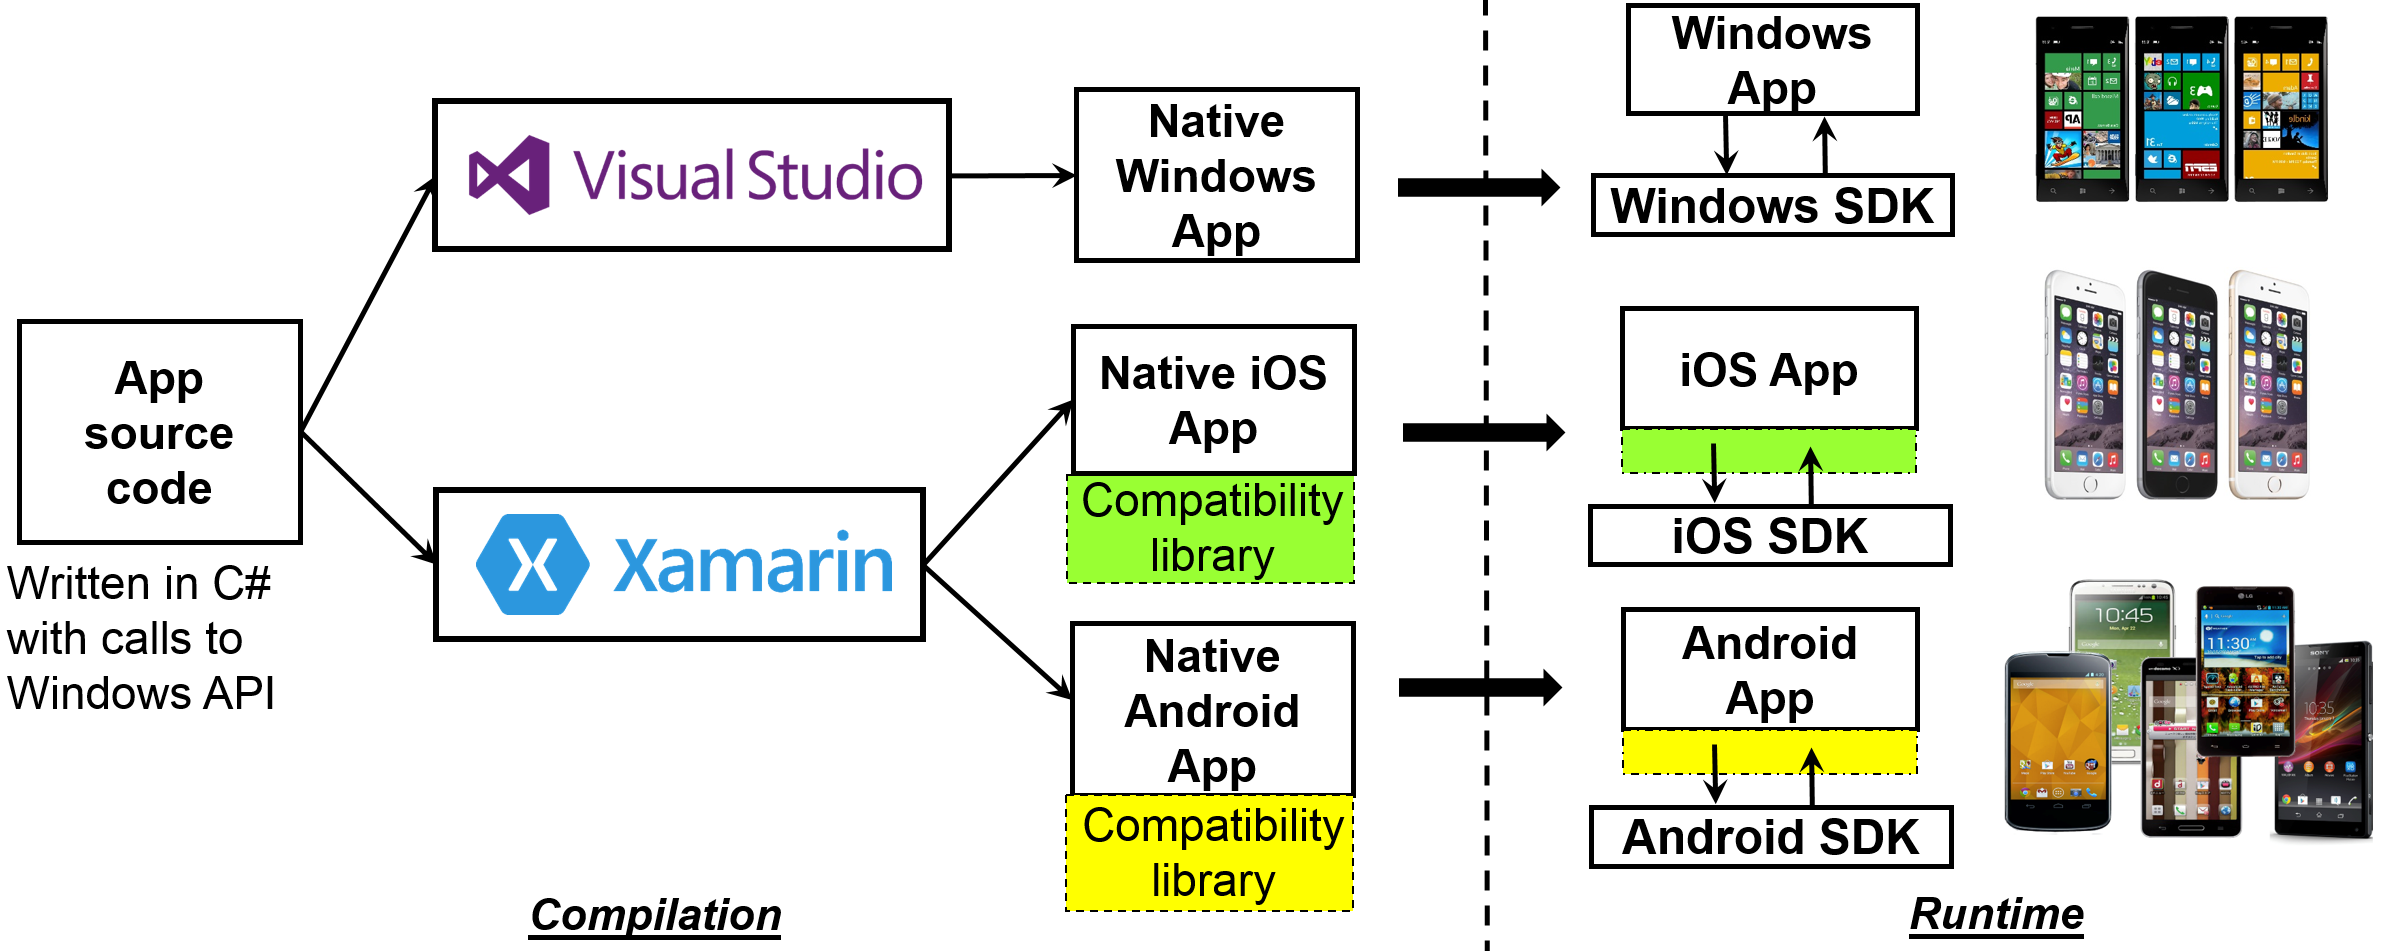
\includegraphics[keepaspectratio=true,width=0.9\textwidth]{figures/xptools-overview.png}
\mycaption{Overall operation of a cross-platform mobile app development
framework, using Xamarin as a concrete example. Developers build apps as they
would for the Windows Phone, in C\# using calls to the API of the Windows Phone
SDK. This code can directly be compiled to Windows Phone apps using the Visual
Studio toolchain. Xamarin allows developers to use the same source code to
build native Android or iOS apps. Xamarin provides compatibility libraries
that translate Windows SDK API calls in the code to the relevant API calls of
the underlying Android and iOS SDKs.}{\label{figure:xplatform-overview}}
\end{figure*}

There are two broad classes of cross-platform frameworks available today.  The
first class, which we call \textit{Web-based frameworks}, allows developers to
build mobile apps using languages popularly used to build Web applications,
such as HTML5, JavaScript, and CSS. Examples of such frameworks include Adobe
PhoneGap~\cite{phonegap}, Sencha~\cite{sencha} and IBM
MobileFirst~\cite{worklight}.  Developers specify the app's logic and user
interface using one or more of the Web-development languages.  However, these
languages do not contain primitives to allow apps to access resources on the
phone, \eg~peripherals such as the camera and microphone, the address book, and
phone settings. Thus, Web-based frameworks provide supporting runtime libraries
that end-users must download and execute on their mobile devices. Mobile apps
interface with these libraries to access resources on the mobile devices---such
mobile apps are also popularly called hybrid mobile apps.  Web-based frameworks
allow developers to rapidly prototype mobile apps.  However, these frameworks
are ill-suited for high-performance apps, such as games or those that use
animation. The expressiveness of the resulting mobile apps is also limited by
the interface exported by the runtime libraries offered by the frameworks.


The second class, which we call \textit{native frameworks}, addresses the above
challenges. Examples of such frameworks include Xamarin~\cite{xamarin},
Apportable~\cite{apportable} and MD$^2$~\cite{md2:sac13,myappconverter}. These
frameworks generally support a \textit{home platform} and one or more
\textit{target platforms}. Developers build mobile apps as they normally would
for the home platform, and leverage the framework's support to automatically
produce apps for the target platforms as well. For example, the home platform
for Xamarin is Windows Phone, and developers build apps using C\# and the API
of the Windows Phone SDK. The Xamarin framework allows developers to
automatically build Android and iOS apps using this code base (see
\figref{figure:xplatform-overview}). Likewise, the home platform for Apportable
is iOS. Developers build apps using Objective-C and the iOS SDK, and leverage
Apportable to produce Android apps from this code base.  In this paper, we will
focus on native frameworks for cross-platform mobile app development. 

When an app developer uses native frameworks, he implicitly expects the apps to
behave consistently across the home and target platforms. Realizing this
expectation depends to a large extent on the fidelity with which the native
framework translates the API calls to SDK of the home platform to the
corresponding SDK of the target platform(s). Unfortunately, this translation is
a complex task because the platform must correctly encode the semantics of both
the home platform and target platform SDK and the relationship between them.
This complexity translates into bugs in the frameworks, \eg~as of mid-December
2014, Xamarin's Bugzilla database shows a history of about 17,600 bug reports,
5,100 of which are still unresolved (listed as ``open'' or ``new''), while
Apportable's bug database shows a history of 820 bug reports, 449 of which are
unresolved.

In this paper, we develop an approach to test native cross-platform app
development tools. Specifically, we aim to discover cases where the behavior of
the application on the home platform is inconsistent with the behavior of its
counterpart on a target platform. Our approach is based on \textit{differential
testing}~\cite{mckeeman:difftest:1998}. We generate random test cases (using
methods described in prior work~\cite{randoop:icse07}), which in our case are
mobile apps in the source language of the home platform. We then use this code
to produce two versions of the app, one for the home platform, and one for the
target platform using the native framework. We then execute the apps and
examine the resulting state for inconsistent behavior.  When two versions of
the app are produced from the same source code, any differences in the behavior
across the versions are indicative of a problem either in the home platform's
SDK, the target platform's SDK, or the way the native framework translates
between the two SDKs.

To realize this approach, we must address two issues::
%
\begin{mylist}
%
\item \textbf{How can we generate effective test cases?} The key research
challenge here is that the space of valid programs that we can generate as test
cases is essentially unbounded. While we could sample from this space, the
effectiveness of these test cases in inducing inconsistent behavior is
questionable.

To address this challenge, we observe that the main difficulty in building
cross-platform mobile app development tools is \textit{translating between the
semantics of the SDKs of the home and target platforms}. Our test-case
generator therefore produces programs that contain random sequences of
invocations to the home platform's SDK. We then observe whether the resulting
apps on the home and target platforms behave consistently. By focusing on the
SDK alone, our approach narrows testing to the most error-prone components of
the cross-platform frameworks.

\item \textbf{How can we check for inconsistent behavior?} Each of our test
cases is compiled into a full-fledged app, one each for the home and target
platforms. When we run the corresponding apps, we must observe their behaviors
to identify inconsistencies. The main research challenge here is in defining a
suitable notion of ``behavior.''

We address this challenge by observing all data structures that are reachable
from the variables defined in the test cases. We serialize these data
structures into a standard format, and compare the serialized versions on the
home and target platforms. Assuming that the state of the home and target
platforms is the same before the test cases are executed, the final state in
each platform after the test cases have been executed must also be the same.
If not, we consider this inconsistent behavior and report an error.
%
\end{mylist}

We have prototyped this approach in a tool called \tool, which we have applied
to test the Xamarin framework using Android as the target platform. Using
\tool, we have found \checkme{47} inconsistencies, which corresponded to bugs
either in Xamarin or the Microsoft SDK (we have reported many of these to
Xamarin or Microsoft). To date, one of these bugs has also been fixed in the
development branch of Xamarin.


\mysection{Introduction}
\label{section:introduction}

% \addtext{Task~0}{Test}
% \deltext{Test}

Personal computing devices, such as phones, tablets, glasses, watches,
assistive health monitors and other embedded devices have become an integral
part of our daily lives. We carry these devices as we go, and expect them to
connect and work with the environments that we visit.

While the increasing capability of smart devices and universal connectivity are
generally desirable trends, there are also environments where these trends may
be misused. In enterprise settings and federal institutions, for instance,
malicious personal devices can be used to exfiltrate sensitive information to
the outside world. In examination settings, smart devices may be used to
infiltrate unauthorized information~\cite{url:examcheating}, surreptitiously
collude with peers~\cite{smartwatch:fc14} and cheat on the exam.  Even in less
stringent social settings, smart devices may be used to record pictures, videos
or conversations that could compromise privacy. We therefore need to regulate
the use of smart devices in such \textit{restricted spaces}.

Society currently relies on a number of \adhoc\ methods for policy enforcement
in restricted spaces. In the most stringent settings, such as in federal
institutions, employees may be required to place their personal devices in
Faraday cages and undergo physical checks before entering restricted spaces.
In corporate settings, employees often use separate devices for work and
personal computing needs. Personal devices are not permitted to connect to the
corporate network, and employees are implicitly, or by contract, forbidden from
storing corporate data on personal devices. In examination settings, proctors
ensure that students do not use unauthorized electronic equipment.  Other
examples in less formal settings include restaurants that prevent patrons from
wearing smart glasses~\cite{url:glassban}, or privacy-conscious individuals who
may request owners to refrain from using their devices.

We posit that such \adhoc\ methods alone will prove inadequate given our
increasing reliance on smart devices. For example, it is not possible to ask an
individual with prescription smart glasses (or any other assistive health
device) to refrain from using the device in the restricted space. The right
solution would be to allow the glass to be used as a vision corrector, but
regulate the use of its peripherals, such as the camera, microphone, or WiFi.
A general method to regulate the use of smart devices in restricted spaces
would benefit both the \textit{hosts} who own or control the restricted space
and \textit{guests} who use smart devices.  Hosts will have greater assurance
that smart devices used in their spaces conform to their usage policies. On the
other hand, guests can benefit from and be more open about their use of smart
devices in the host's restricted space.\footnote{We only consider overt use of
guest devices.  Covert use must still be addressed using other methods, such as
physical checks.}

Prior research projects
(\eg~\cite{asm:sec14,flaskdroid:sec13,conxsense:asiaccs14,worlddriven:ccs14,blindspot:2009,markit:upside14})
and enterprise mobile-device management (MDM) solutions to address this problem
(\eg\ Samsung Knox~\cite{knox:mdm}, Microsoft Intune~\cite{ms:intune} and
Blackberry EMM~\cite{blackberry:emm}) have typically assumed that guest devices
are benign. These solutions outfit the guest device with a security-enhanced
software stack that is designed to accept and enforce policies supplied by
restricted space hosts. A host must trust the software running on a guest
device to correctly enforce its policies, and generally has no means to obtain
guarantees that a guest device is policy-compliant.  Clearly, malicious guest
devices with a suitably-modified software stack can easily bypass policy
enforcement.

Our vision is to enable restricted space hosts to enforce usage policies on
guest devices with provable security guarantees. Simultaneously, we also wish
to reduce the amount of trusted policy-enforcement code (\ie~the size of the
security-enhanced software stack) that needs to execute on guest devices. To
that end, this paper offers a number of advances:

\begin{mylist}
%
\item \emphitem{Use of trusted hardware.} We leverage the ARM
TrustZone~\cite{armtz} on guest devices to offer provable security guarantees.
In particular, a guest device uses the ARM TrustZone to produce
\textit{verification tokens}, which are unforgeable cryptographic entities that
establish to a host that the guest is policy-compliant.  Malicious guest
devices, which may have violated the host's policies in the restricted space,
will not be able to provide such a proof, and can therefore be apprehended by
the host. Devices that use the ARM TrustZone are now commercially available and
widely deployed~\cite{knox:ccs14}, and our approach applies to these devices.
%
\item \emphitem{Remote memory operations.} We use host-initiated remote memory
operations as the core method to regulate guest devices. In this approach, a
host decides usage policies that govern how guest devices must be regulated
within the restricted space. For example, the host may require certain
peripherals on the guest device (\eg~camera, WiFi or 3G/4G) be disabled in the
restricted space. The host sends these policies to the guest device, where a
trusted policy-enforcement mechanism applies these policies by reading or
modifying device memory. 

The principal benefit of using remote memory operations as an API for policy
enforcement is that it considerably simplifies the design and implementation of
the policy-enforcement mechanism, while still offering hosts fine-grained
control over guest devices.  Remote memory operations also give hosts that use
our approach the unique ability to scan guest devices for kernel-level malware.
Combined with the ARM TrustZone, which helps bootstrap trust in the guest's
policy-enforcement code, our approach offers hosts an end-to-end assurance that
guest devices are policy-compliant.
%
\item \emphitem{Secure device checkpointing.} The downside to enforcing
policies by modifying device memory is that changes to the guest device are
ephemeral, and can be undone with a simple reboot of the guest device. We
therefore introduce \textit{REM-suspend}, a secure checkpointing scheme to
ensure that a guest device remains ``tethered'' to the host's policies even
across device reboots and other power-down events.
%
\item \emphitem{Vetting for guest device privacy and security.} The advances
above benefit hosts, but guests may be uncomfortable with the possibility of
hosts accessing and modifying raw memory on their devices. If access to raw
guest device memory is not mediated, malicious hosts may be able to use this
access to compromise the guest's privacy and security. For example, the host
can read sensitive and private app data from devices and install malicious
snooping software (\eg~keyloggers) on the guest device.  We therefore mediate
the host's access to the guest device by introducing a vetting service. The
vetting service is trusted and configurable by guests, and allows them to check
the safety of the host's memory operations before performing them on the
devices.  The vetting service ameliorates guests' privacy and security concerns
and restricts the extent to which hosts can control their devices.
%
\end{mylist}

We built and evaluated a prototype to show the benefits of our approach. We
show that a small policy-enforcing code base running on guest devices offers
hosts fine-grained policy-based control over the devices. We also show that a
vetting service with a few simple sanity checks allows guests to ensure the
safety of the host's remote memory operations.


% \mysection{Restricted Space Usage Model}
\label{section:usagemodel}

We now provide an overview of the restricted space model, motivate some
features of our enforcement mechanism, and describe our threat model.

\subsection{Overall Workflow}

\myparagraph{Check-in}
As depicted in \figref{figure:restrictedspaces}, when a guest enters a
restricted space in which he wishes to use his devices, he ``checks-in'' each
of his devices during entry. During check-in, the guest device communicates
with the host's policy server for the following tasks:

\begin{mylist}
%
\item \textit{Authentication.} The authentication step allows the guest and
host to mutually identify each other. We assume that both the guest and the
host have cryptographic credentials (\eg~public/private key pairs) that can be
validated via a trusted third party, such as a certifying authority. The host
and the guest mutually authenticate each other's credentials in the standard
way, for example, as is typically done during SSL/TLS handshakes.

The host's policies are enforced by a mechanism that executes in the guest.  As
previously discussed, this mechanism is part of the TCB, and must therefore not
be tampered by the guest.  We rely on secure hardware on the guest device (the
ARM TrustZone) to ensure this property.  In particular, we rely on the secure
hardware to detect and prevent any attempts to tamper with the TCB on the
guest. This can be ensured using a special boot-time protocol implemented atop
the secure hardware.

It is important to note that this TCB is \textit{not} the end-user's usual work
environment on the device, \eg~the traditional Android, iOS or Windows
environment with apps. Rather, the TCB is an environment that is created and
distributed by a trusted entity, such as the device vendor, and executes in
isolation on the guest device. 

% NOTE: Clarification from Ferdinand -- this is not how attestation works on
% the TZ as there is no hardware root of trust on the device. Rather vendors
% lock down the secure world and implement secure boot within it.
%
% The host checks the trustworthiness of the TCB by attesting the software
% stack that executes the policy enforcement mechanism.  This attestation is
% typically done from the hardware-up, and is used to ensure that the TCB
% booted correctly and only executes software components that can be trusted by
% the host.  
%
% We can therefore assume that the correct configurations of the TCB are
% well-known to the host, thereby enabling attestation. As we will describe in
% \sectref{section:mechanism}, our TCB on guest devices is simple in its
% functionality and small in size. We attest this TCB using trusted hardware on
% the guest device (the ARM TrustZone) as the root of trust, but other
% implementations may be possible.

\item \textit{Host analyzes device.} The host leverages the TCB to analyze the
guest device. Our mechanism allows hosts to \textit{remotely fetch memory
pages} (and CPU register state) belonging to the guest device.  The TCB
computes a cryptographic checksum over the memory pages to ensure that they are
not tampered with as they are transferred from the guest to the host. 

The host uses raw memory pages from the device in two ways. First, it scans
memory pages to ensure that the device is free of malicious software, \eg~in
the form of malicious apps or kernel modules.  Second, it extracts
configuration information from the device. This includes the kernel version,
the list of peripherals supported by the device, memory addresses of various
device drivers for peripherals on the device and the state of these peripherals
(\eg~whether a certain peripheral is enabled and its settings). The host can
also checkpoint the state of these peripherals so that they can be restored at
check-out. 

\item \textit{Host modifies guest's configuration.} The host modifies the guest
device's configuration to conform to its restricted usage policies.  In the
example shown in \figref{figure:restrictedspaces}, the host's policy is to
disable the camera and the 3G/4G data plan on all devices. The host enforces
this policy by creating a sequence of \textit{remote memory writes} that
directly modify the memory state of the device. For example, the host could
prevent the use of the camera and 3G/4G data plan by unlinking the device
drivers corresponding to the camera and the modem. The host uses the
configuration information extracted in the previous step to determine the
memory addresses that must be modified to unlink these drivers. 

We assume that it is the host's responsibility to ensure that these
configuration modifications are not easily bypassable. For example, these
modifications may be undone if the user of the guest device can directly modify
kernel memory, \eg~by dynamically loading kernel modules or using
\code{/dev/kmem} in the end-user's work environment. The host must use the
inspection phase to identify device configurations that could lead to such
attacks, and disallow the use of such devices in the restricted space.

\item \textit{Host obtains verification token from guest.} After the guest
device has been configured, the TCB produces a \textit{verification token} to
be transmitted to the host. The verification token is an unforgeable value that
encapsulates the set of configuration changes to the device. The TCB computes
the token as a checksum over the memory locations that were modified.  The
token is unforgeable in that only the TCB can re-create its value as long as
the device configuration has not been altered, and any malicious attempts to
modify the token can be detected by the TCB and the host.

At any point when the device is in the restricted space, the host can request
the TCB on the device to send it the verification token. The TCB computes this
token afresh, and transmits it to the host,\footnote{This assumes that the
host's policy still allows a communication channel between the host and the
guest. If all of the guest's peripherals are disabled, the host will need
physical access to the guest to visually obtain the freshly-computed
verification token.} which compares this freshly-computed token with the one
obtained during check-in. It can use this comparison to ensure that the guest
has not altered the device configurations from the previous step.  The
verification token is ephemeral, and can be computed afresh by the guest only
within an expiration period.  In our prototype, the TCB cannot recompute the
verification token if the guest device is rebooted, thereby ensuring that
end-users cannot undo the host's configuration changes by simply rebooting the
device.
%
\end{mylist}

\myparagraph{Check-out}
Once checked-in, the guest device can freely avail of the facilities of the
restricted space under the policies of the host. For example, in
\figref{figure:restrictedspaces}, the smart glass can pair with the smart phone
via Bluetooth, while the smart phone can connect to and use the host's WiFi
access point. When the guest exits the restricted space, he checks-out the
device, accomplishing two goals: 
%
\begin{mylist}
%
\item \textit{Host checks guest state.} The host checks guest device's
configuration by requesting the verification token from the device's TCB to
ensure that the configuration has not been altered. If it finds that the
verification token does not match the value obtained from the device at
check-in, it can detain the device for further inspection, \eg~to determine
whether any data from the restricted environment was exfiltrated.

Note that it is not usually possible to differentiate between mismatches that
happen because of benign reasons, such as a device reboot, or malicious ones,
such as when an end-user intentionally modified the peripheral configurations
required by the host. This is because even malicious modifications can be
masked by simply rebooting the device, and making the mismatch seem benign.
Thus, the host's policy to deal with mismatches depends upon the sensitivity of
the restricted environment. For example, in a federal setting, a detailed
forensic examination of the device may be necessary, the possibility of which
could deter a malicious guest from bypassing the host's policy enforcement. As
previously discussed, hosts can request the verification token from the device
at any time when it is in the restricted space. Hosts can use this feature to
frequently check the verification token and narrow down the timeframe of the
violation.

\item \textit{Restoring guest state.} To restore the state of the device, the
end-user could simply reboot the device. The host only modifies the memory of
the device, and not persistent storage. Rebooting therefore undoes all the
memory modifications performed by the host and boots the device from an
unmodified version of the kernel in persistent storage. Alternatively, the host
can restore the state of the guest device's peripherals from a checkpoint
created at check-in. The main challenge here is to ensure consistency between
the state of a peripheral and the view of the peripheral from the perspective
of user-level apps. For example, when the 3G interface is disabled, an app
loses network connectivity. However, because we only modify memory and do not
actually reset the peripheral, the 3G card may have accumulated packets, which
the app may no longer be able to process when the kernel state is restored.
Mechanisms such as shadow drivers~\cite{shadow:tocs06} can enable such ``hot
swaps'' of kernel state, enabling guest devices to continue without
rebooting.
%
\end{mylist}

% \todo{VG}{A security analysis here? -- No need. Fold in any security
% arguments with the corresponding step in the workflow.}

\subsection{Malicious Hosts} 
\label{section:usagemodel:malicious}
%
Our discussion so far has assumed that hosts are benign. Authentication at
check-in ensures that remote access to guest device memory is available only to
hosts that the guest approves. However, it may be possible even for such hosts
to misuse the facilities of our mechanism to violate the security and privacy
of the guest. For example, a malicious host could use remote memory reads to
obtain the guest's personal data. It could also install a key logger or a
backdoor to spy on the guest's activities. Even if the host is not overtly
malicious, it is possible that the configuration changes that it makes will
render the guest's device vulnerable to attacks. This is reminiscent of the
2006 incident when CD DRM software installed by Sony made the systems on which
it was installed vulnerable to certain kinds of attacks~\cite{sonydrm:sec06}.

To protect guest devices from malicious hosts, we provide a \textit{trusted
vetting service}. We assume that guests register their device(s) with the
vetting service beforehand. When the host sends a remote read/write request,
the guest device forwards the request to the service together with its current
memory configuration. The vetting service analyzes the requests against the
memory configuration and determines whether the request conforms to certain
safety policies. \sectref{section:vetting} presents the details of our vetting
service.

The vetting service could directly be implemented in the TCB executing on the
guest device, but this has the undesirable effect of bloating the TCB on the
device. We therefore implement vetting as a cloud service.  Note that vetting
is optional. If the guest trusts the host, it could carry out the host's
requests without vetting.

% It is challenging to protect guest devices from malicious hosts, and
% \textit{for this paper, we will assume that hosts are benign}. Nevertheless,
% there are a few defenses that could be used to protect against malicious
% hosts.  To protect personal data, privacy-conscious users could store their
% data encrypted on disk and in memory, except when it is used. However, this
% would require apps on the device to be redesigned to be aware of such
% encrypted data.

% To protect against remote writes that maliciously modify the guest device
% (\eg~by installing a keylogger), the guest could rely on a trusted third
% party to vet the operations of the host. That is, the guest could forward its
% memory configuration and the remote operations requested by the host to the
% trusted third party prior to making any memory modifications. The guest would
% proceed with the modifications only if the trusted third party certifies that
% the operations do not install malicious software on the guest device.
% Alternatively, a simpler solution is to restrict the kinds of remote write
% operations that a host can initiate. For example, the TCB could enforce that
% the only remote memory writes available to the host are writing \textsc{null}
% bytes to memory locations that store device driver hooks. This would allow
% hosts to unlink drivers and disable peripherals, but prevent them from
% installing malicious software.

\subsection{Covert Use and Legacy Devices}
%
It is certainly possible for a guest to bypass the host's policies by not
declaring a device during check-in, and using it covertly within the restricted
space. As long as the guest carefully configures the device to avoid accessing
any of the host's resources in the restricted space, \eg~its WiFi access
points, and remain stealthy, the device cannot be detected by the host.

Our focus in this paper is to address policy enforcement for overt uses of
smart devices. Covert uses, such as the above, are out of the scope of the
mechanisms developed in this paper. Instead, we assume that traditional methods
such as physical security checks are necessary to detect covertly-hidden
devices.

Finally, what if the guest uses a ``legacy'' device, \ie~one that is not
equipped with trusted hardware, such as the ARM TrustZone? In
\sectref{section:discussion}, we present a number of design alternatives to
enforce policies on such legacy devices.  However, because they do not use
secure hardware, these alternatives cannot offer the same security guarantees
as our approach, or require larger TCBs on guest devices to offer similar
guarantees. Our take on the issue of legacy device support is that while legacy
devices are certainly important in today's settings, we are beginning to see an
increasing deployment of devices equipped with trusted hardware
(\eg~see~\cite{knox:ccs14}). We hypothesize that moving forward, hosts will
have to contend with fewer legacy guest devices than they do today.

\subsection{Threat Model} 
\label{section:threat}
%
Given the discussion in this section, we now summarize our threat model. 
Each guest device is assumed to be partitioned into two parts: (1)~the
end-user's work environment, and (2)~the environment that runs the policy
enforcement mechanism. 

From the perspective of the host, the end-user's work environment is untrusted.
The host must trust the policy enforcement mechanism, but because it executes
on the guest device, the host leverages secure hardware, the ARM TrustZone in
our case, to bootstrap this trust. Having established trust, the host then uses
the policy enforcement mechanism to securely read and modify the memory state
of the work environment. It is the host's responsibility to inspect the memory
state of the work environment to determine whether it is malicious, contains
known exploitable vulnerabilities, or allows guests to bypass the configuration
changes that the host may make.  Once the host determines that the guest's work
environment is acceptable, it can induce changes to the guest's memory state.
Guests are assumed to keep their devices powered on for the duration of their
stay in the restricted space, failing which the verification tokens will no
longer match. Mismatches may also happen if the guest maliciously modifies the
host's changes.

The work environment may contain zero-day vulnerabilities, such as a
newly-discovered buffer overflow in the kernel. The host may not be aware of
this vulnerability, but a malicious guest may know of it and have an exploit to
bypass the host's policies.  Such threats are outside the scope of our work,
but the host may protect itself by requiring the guest's work environment to
run a fortified software stack (\eg~Samsung Knox~\cite{knox:ccs14} or
MOCFI~\cite{mocfi:ndss12}). The host can check this requirement during the
inspection phase. A malicious work environment may also launch a
denial-of-service attack, which will prevent the host from communicating with
the TCB on the guest device.  However, such attacks can readily be detected by
the host, which can then prevent the device from entering the restricted space.
We exclude such attacks from our threat model.

From the perspective of the guest, if the host is untrusted, it can rely on a
trusted vetting service to determine if the host's read and write requests are
safe.

% the host is assumed to only make benign changes to the guest work
% environment.  However, it may be possible to relax this assumption provided
% the guest vets all the host's intended changes with a trusted third party.
% Similarly, although the host is assumed not to maliciously compromise the
% guest's privacy, a guest may choose to encrypt its in-memory and on-disk data
% to protect it from the host.


% What if kernel module is loaded dynamically? We disable that.





\begin{figure*}[t!]
\centering
\begin{tabular}{ccc}
\begin{minipage}{0.46\textwidth}
\centering
\begin{tabular}{|c|}
\hline
\indent\vspace{-0.0cm}\\
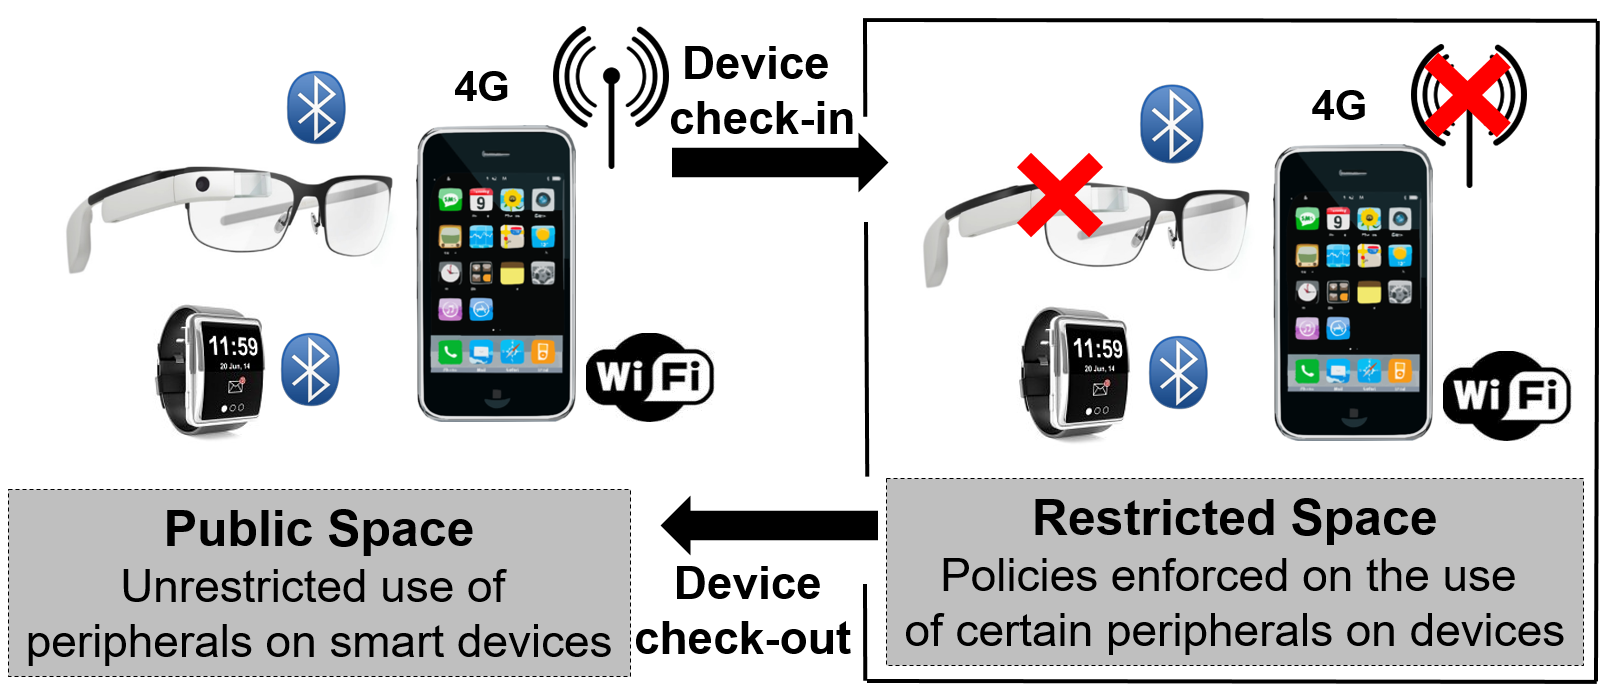
\includegraphics[keepaspectratio=true,width=0.95\textwidth]{restricted-space.png}\\
\multicolumn{1}{|p{0.98\textwidth}|}
{\small {\bf Restricted space model.} Guests ``check-in'' their personal
devices when entering restricted spaces. During check-in, hosts inspect,
analyze and modify the configurations of these devices in accordance with their
usage policies. In this example, the host restricts the use of the camera on
the smart glass, and the 4G data interface on the smart phone. However, the
glass and watch can continue to use Bluetooth pairing, while the phone can
connect to the host's access points using WiFi.  When guests leave the
restricted space, they ``check-out'' their devices, restoring them to their
original configurations.}\\
\hline
\end{tabular}
\end{minipage} & & 
\begin{minipage}{0.46\textwidth}
\centering
\begin{tabular}{|c|}
\hline
\indent\vspace{-0.2cm}\\
\includegraphics[keepaspectratio=true,width=0.90\textwidth]{host-guest.png}\\
\indent\vspace{-0.5cm}\\
\multicolumn{1}{|p{0.98\textwidth}|}
{\small {\bf Guest device setup.} Guest devices are equipped with ARM TrustZone
and execute components of the policy enforcement mechanism in the secure world
(SW). The details of this mechanism appear in \sectref{section:mechanism}.  At
check-in, the host's policy server leverages the secure world to remotely
inspect and modify normal world (NW) memory.}\\
\hline
\end{tabular}
\end{minipage}
\end{tabular}
%\indent\vspace{-0.5cm}
\mycaption{An overview of the entities of our restricted space model and the
setup of guest devices.}
{\label{figure:restrictedspaces}}
\end{figure*}

\mysection{Restricted Spaces}
\label{section:usagemodel}

We provide an overview of the restricted space model, motivate some features of
our enforcement mechanism, and describe our threat model. Because our mechanism
relies on the ARM TrustZone, we begin by introducing its features.

\subsection{Background on the ARM TrustZone}
\label{section:armback}

The TrustZone is a set of security enhancements to chipsets based on the ARM
architecture. These enhancements cover the processor, memory and peripherals.
With TrustZone, the processor executes instructions in one of two security
modes at any given time, a \textit{normal world} and a \textit{secure world}. A
third \textit{monitor mode} facilitates switching between the normal and the
secure worlds.  The secure and normal worlds have their own address spaces and
different privileges.  The processor switches from the normal world to the
secure world via an instruction called the secure monitor call (\textsf{smc}).
When an \textsf{smc} instruction is invoked from the normal world, the
processor context switches to the secure world (via monitor mode) and freezes
execution of the normal world.

The ARM TrustZone partitions memory into two portions, with one portion
being exclusively reserved for the secure world. It also allows individual
peripherals to be assigned to the secure world.  For these peripherals,
hardware interrupts are directly routed to and handled by the secure world.
While the normal world cannot access peripherals or memory assigned to the
secure world, the secure world enjoys unrestricted access to all memory and
peripherals on the device. It can therefore access the code and data of the
normal world. The secure world can execute arbitrary software, ranging from
simple applications to an entire operating system (OS).
%
% NOT the CPU state. Registers are "banked", and only monitor mode can view
% them all.

A device with ARM TrustZone boots up in the secure world. After the secure
world has initialized, it switches to the normal world and boots the OS there.
Most TrustZone-enabled devices are configured to execute a \textit{secure boot}
sequence that incorporates cryptographic checks into the secure world boot
process~\cite[\S5.2.2]{armtz}. For example, the device vendor signs the code
with its private key, and the vendor's code in the boot ROM verifies this
signature using the vendor's public key. These checks ensure that the integrity
of the boot-time code in the secure world has not been compromised, \eg~by
reflashing the image on persistent storage. Most vendors lock down the secure
world via secure boot, thereby ensuring that it cannot be modified by
end-users. This feature allows hosts to trust software executing in the secure
world and treat it as part of the trusted computing base (TCB). In this paper,
we assume that guest devices use secure boot.

\subsection{Entering and Exiting Restricted Spaces}
\label{section:usagemodel:checkin}

\myparagraph{Check-in} When a guest enters a restricted space, he checks in
each of his devices during entry (\figref{figure:restrictedspaces}).  During
check-in, the guest device communicates with the host's policy server for the
following tasks:

\begin{mylist}
%
\item \emphitem{Authentication.} The first step is for the host and the guest to
mutually identify each other. We assume that both the guest and the host have
cryptographic credentials (\eg~public/private key pairs) that are validated
via a trusted third party, such as a certifying authority. The host and the
guest mutually authenticate each other's credentials in the standard way, as is
done during SSL/TLS handshakes.

The host's policies are enforced by a mechanism that executes in the secure
world of the guest device. We rely on TrustZone's secure boot sequence to
prevent unauthorized modifications to this code. Note that the end-user's usual
work environment on the device, \eg~the traditional Android, iOS or Windows
environment with apps, executes in the normal world (and is untrusted). We
expect the secure world software running the mechanisms proposed in this paper
to be created and distributed by trusted entities, such as device vendors, and
execute in isolation on guest devices.

\item \emphitem{Host remotely reads guest state.} The host requests the guest
device for a snapshot of its normal world memory and CPU register state. The
secure world on the device fulfills this request (after it has been cleared by
the vetting service) and sends it to the host. The secure world also sends a
cryptographic checksum of this data to prevent unauthorized modifications
during transit.

The host uses raw memory pages from the device in two ways. First, it scans
memory pages to ensure that the normal world kernel is free of malicious
software. A clean normal world kernel can bootstrap additional user-level
security mechanisms, \eg~an antivirus to detect malicious user-level apps.
Second, it extracts the normal world's configuration information. This includes
the kernel version, the list of peripherals supported, memory addresses of
various device drivers for peripherals and the state of these peripherals
\eg~whether a certain peripheral is enabled and its settings. The host can also
checkpoint the configuration for restoration at check-out. 

\addtext{Task 7}{The host terminates check-in at this point if it finds that
the guest device is malicious or runs a kernel version that it cannot
reconfigure. The action that the host takes depends upon the specific setting.
For example, in a federal building, the device owner may be asked to quarantine
the device outside the restricted space or enclose it in a physically-secured
Faraday cage. In less stringent settings, the host may blacklist the device's
MAC address and prevent it from connecting to any local resources in the
restricted space. Note that benign end-users may not have willingly installed
malware on their devices. A failed check-in has the desirable side-effect of
allowing such end-users to detect that their device is infected.}

\item \emphitem{Host remotely modifies guest state.} The host modifies the guest
device to conform to its restricted usage policies.  The host's restrictions on
a guest device depend on what it perceives as potential risks.  Cameras and
microphones on guest devices are perhaps the most obvious ways to violate the
host's confidentiality because they can be used to photograph confidential
documents or record sensitive meetings. Networking and storage peripherals such
as WiFi, 3G/4G, Bluetooth and detachable storage dongles can work in concert
with other peripherals to exfiltrate sensitive information. Dually, guest
devices can also be used to infiltrate unauthorized information into restricted
spaces, \eg~students can cheat on exams by using their devices to communicate
with the outside world.

The host controls peripherals on guest devices by creating a set of updates to
the device's normal world memory and requesting the secure world to apply them.
For example, one way to disable a peripheral is to unlink its driver from the
device's normal world kernel (details in \sectref{section:policy}).  The secure
world applies these updates after using the vetting service to ensure the
safety of the requested updates.

We assume that it is the host's responsibility to ensure that the memory
modifications are not easily bypassable. For example, they may be undone if the
user of the guest device directly modifies kernel memory, \eg~by dynamically
loading kernel modules or using \textsf{/dev/kmem} in the normal world. The
host must inspect the guest device's snapshot for configurations that lead to
such attacks, and disallow the use of such devices in the restricted space.

In steps \circtwo\ and \circthree, the secure world performs the host's read
and write operations only if they are approved by the vetting service. Guests
configure the vetting service to suit their security and privacy goals. If the
vetting service deems an operation unsafe, device check-in is aborted and the
device is left unmodified. The guest cannot use the device in the restricted
space because its security and privacy goals conflict with the host's usage
policies.

\item \emphitem{Host obtains verification token from guest.} After the guest
device state has been modified, its secure world produces a verification token
to be transmitted to the host. The verification token is a cryptographic
checksum over the memory locations that were modified. The token is unforgeable
in that only the secure world can re-create its value as long as the host's
memory updates have not been altered, and any malicious attempts to modify the
token can be detected by the secure world and the host.

\addtext{Task 5}{The check-in steps above bear some resemblance to TPM-based
software attestation protocols developed in the trusted computing
community~\cite{Sailer04}. Like TPM measurements, which attest the software
stack or properties of dynamic data structures~\cite{sadeghi:isc08},
verification tokens attest that a guest device's state complies with the host's
policies. Both TPM measurements and verification tokens are grounded in a
hardware root of trust.  However, unlike traditional software attestation,
which has largely been restricted to passive checks of a remote machine's
state, verification tokens attest to the integrity of the host's remote
modifications of the guest device.}

\addtext{Task 1}{Like in software attestation, a correct verification token
attests the state of the guest device only at the instant at which it was
produced by the secure world. To ensure that the guest device remains
policy-compliant, the host can request the device to send it the verification
token at any point when the device is in the restricted space.} 
The secure world on the device computes this token afresh, and transmits it to
the host,\footnote{This assumes that the host's policy still allows
communication between the host and the guest. If all of the guest's peripherals
are disabled, the host must physically access the guest to visually obtain the
fresh token.} which compares this freshly-computed token with the one obtained
during check-in. It uses this comparison to ensure that the guest has not
altered the normal world memory updates from the previous step. The
verification token incorporates a host-supplied challenge to ensure that the
guest device cannot simply replay old tokens. 
\addtext{Task 1}{As we demonstrate in \sectref{section:evaluation},
verification tokens are only a few hundred bytes in size and can be computed by
the secure world in just a few milliseconds. Thus, hosts can request guest
devices to send verification tokens at frequent intervals, thereby increasing
confidence that the guest device was continuously policy-compliant.}

The verification token is ephemeral, and can be computed afresh by the guest
only within an expiration period. The token expires upon device check-out or if
the device is powered off, thereby ensuring that end-users cannot undo the
host's memory updates by simply rebooting the device.  In
\sectref{section:mechanism:REMsuspend}, we describe
\textit{\underline{re}stricted space-\underline{m}ode (REM) suspend}, a special
protocol that suspends the device while allowing the verification token and the
host's memory updates to persist.
%
\end{mylist}

\myparagraph{Check-out} Once checked-in, the guest device are free to avail of
the facilities of the restricted space under the policies of the host. For
example, in \figref{figure:restrictedspaces}, the smart glass and watch can
pair with the smart phone via Bluetooth, while the smart phone can use the
host's WiFi access point. When the guest checks-out, two tasks must be
accomplished:
%
\begin{mylist}
%
\item \emphitem{Host checks guest state.} The host requests the guest to send
the verification token to ensure that the device is policy-compliant. The token
may not match the value obtained from the device at check-in if the host's
memory modifications have been maliciously altered or if the end-user chose to
consciously bypass REM-suspend and reboot the device.  It is not possible to
differentiate between these cases, and the host's policy to deal with
mismatches depends upon the sensitivity of the restricted environment. For
example, in a federal setting, detailed device forensics may be necessary. As
previously discussed, hosts can request the verification token from the device
at any time when it is in the restricted space. Hosts use this feature to
frequently check the verification token to narrow the timeframe of the
violation.

\item \emphitem{Restoring guest state.} To restore the state of the device, the
end-user simply performs a traditional device reboot. The host only modifies
the memory of the device, and not persistent storage. Rebooting therefore
undoes all the memory modifications performed by the host and boots the device
from an unmodified version of the kernel in persistent storage. Alternatively,
the host can restore the state of the device's peripherals from a checkpoint
created at check-in. The main challenge here is to ensure consistency between
the state of a peripheral and the view of the peripheral from the perspective
of user-level apps. For example, when the 3G interface is disabled, an app
loses network connectivity. However, because we only modify memory and do not
actually reset the peripheral, the 3G card may have accumulated packets, which
the app may no longer be able to process when the kernel state is restored.
Mechanisms such as shadow drivers~\cite{shadow:tocs06} can possibly enable 
such ``hot swaps'' of kernel state and avoid a device reboot.
%
\end{mylist}

\subsection{Threat Model} 
\label{section:threat}
%
We now summarize our threat model. From the host's perspective, the guest
device's normal world is untrusted. However, the host trusts device
manufacturers and vendors to equip the secure world with TrustZone's secure
boot protocol. This allows the host to establish trust in the secure world,
which contains the policy-enforcement code. It is the host's responsibility to
inspect the normal world memory snapshot to determine whether it is malicious,
contains known exploitable vulnerabilities, or allows guests to bypass its
memory modifications.  From the guest device's perspective, the host may
attempt to violate its security and privacy by accessing and modifying normal
world memory. The guest relies on the vetting service, which it trusts, to
determine the safety of the host's remote memory operations. Guests must keep
their devices powered-on or use REM-suspend to ensure that verification
tokens persist during their stay in the restricted space.

\myparagraph{Out-of-Scope Threats} The guest device's normal world may contain zero-day
vulnerabilities, such as a new buffer overflow in the kernel.  The host may not
be aware of this vulnerability, but a malicious guest may have a successful
exploit that allows the host's policies to be bypassed. While such threats are
out of scope, the host may require the guest's normal world to run a fortified
software stack (\eg~Samsung Knox~\cite{knox:ccs14} or
MOCFI~\cite{mocfi:ndss12}) that implements defenses for common classes of
attacks. The host could check this requirement during the inspection phase. A
malicious guest device may also launch a denial-of-service attack, which will
prevent the host from communicating with the secure world on the guest device.
Such attacks can be readily detected by the host, which can prevent the device
from checking-in. We also do not consider physical attacks whereby an
adversarial guest attempts to bypass the host's memory updates by modifying the
contents of the device's memory chip using external methods.

We restrict ourselves to guest devices that use the ARM TrustZone. It may still
be possible for hosts to enforce usage policies on non-TrustZone devices using
other means (see \sectref{section:related}). However, it is not possible to
provide strong security guarantees without trust rooted in hardware. While such
``legacy'' devices are still pervasive today, modern devices are outfitted with
the TrustZone, and data from Samsung~\cite{knox:ccs14} indicates that millions
of ARM TrustZone devices are already deployed. We hypothesize that in the
future, hosts will have to contend with fewer legacy guest devices than they do
today.

% We only consider adversarial guests that attempt to bypass the host's policy
% enforcement via software-based methods from within the normal-world kernel.
% Specifically, we do not consider physical attacks, whereby a guest attempts to
% subtly bypass a host's memory updates by physically modifying the contents of
% the memory chip (and reverting these updates whenever the host requests
% verification tokens).

Finally, we only consider overt uses of guest devices in restricted spaces.
Covert uses, where a guest stealthily smuggles a device into the restricted
space without check-in and carefully avoids an electronic footprint (\eg~by
shielding the device from the host's WiFi access points), must still be
addressed with traditional physical security methods.

% \mysection{Remote Memory Operations}
\label{section:policy}

We now discuss how hosts can use remote memory read and write operations to
analyze and control guest devices.

\myparagraph{Analysis of Guest Devices}
%
A host can analyze memory snapshots of a guest's normal world kernel to
determine its configuration and scan it for kernel malware (also called
kernel-level \textit{rootkits}).

\begin{mylist}
%
\item \emphitem{Retrieving configuration information.} The host can determine the
kernel version by inspecting code pages, thereby also allowing it to check if
the guest has applied recommended security patches. The host can compare a hash
of each kernel code page against a whitelist, \eg~of code pages in approved
Android distributions, to ensure that the normal world is free of malicious
kernel code~\cite{patagonix:sec08,secvisor:sosp07}. Additionally, the host can
ensure that the kernel is configured to disallow well-known attack surfaces,
\eg~access to \textsf{/dev/kmem} and dynamic module loading. Finally, the host
can identify addresses at which functions of a peripheral's driver are loaded,
where they are hooked into the kernel and the addresses that store
memory-mapped peripheral settings. To do so, it can use the recursive memory
snapshot traversal technique described below. The host can use this information
to design the set of memory updates that reconfigure the device to make it
policy-compliant.
%
\item \emphitem{Detecting malicious data modifications.} Rootkits can achieve
malicious goals by modifying key kernel data
structures~\cite{sbcfi:ccs07,shadows:oakland07,specmon:usenix06}.  The attack
surface exposed by kernel data structures is vast.  For instance, a rootkit
could inject a device driver in kernel memory and modify kernel function
pointers to invoke methods from this driver.  Other examples of data structures
that can be misused include process lists, entropy pools used by the kernel's
random number generator, and access control
structures~\cite{shadows:oakland07,specmon:usenix06}.  
%
\end{mylist}

We now describe a generic approach, developed in prior
work~\cite{sbcfi:ccs07,gib:tdsc11,kop:ccs09,kop:sec12,osck:asplos11}, that
hosts can use to detect such malicious data modifications by analyzing the
normal world's memory snapshot. The main idea is to recursively traverse the
memory snapshot and reconstruct a view of the kernel's data structures, and use
this view to reason about the integrity of kernel data. We assume that the host
has access to the type declarations of the data structures used by the guest
device's normal world kernel, \eg~the sizes, layouts, and fields of every data
structure. The host obtains this information from trusted repositories using
the kernel version, extracted as discussed earlier.

Snapshot traversal starts from well-known entrypoints into the system's memory,
\eg~the addresses of the entities in \textsf{System.map}. When the traversal
process encounters a pointer, it fetches the memory object referenced by the
pointer and recurses until all objects have been fetched.  Having reconstructed
a view of kernel data structures, the host can then determine whether they have
been maliciously modified. For example, it could check that function pointers
in the kernel point to functions defined in the kernel's code
space~\cite{sbcfi:ccs07}. Similarly, the host can check that the kernel's data
structures satisfy invariants that typically hold in an uncompromised
kernel~\cite{gib:tdsc11}. We do not further elaborate on specific rootkit
detection policies because they are orthogonal to our focus.

A rootkit-infected OS kernel can be reliably diagnosed \textit{only by
externally observing its code and data}, \eg~using memory snapshots as already
discussed. Prior techniques that enforce policies on guest devices using
security-enhanced, policy-enforcing normal world kernels
(\eg~\cite{asm:sec14,flaskdroid:sec13,conxsense:asiaccs14,worlddriven:ccs14,blindspot:2009,markit:upside14,knox:mdm,ms:intune,blackberry:emm})
can also benefit from our approach to establish normal world kernel integrity
to hosts.

We have restricted our discussion to an analysis of the normal world's kernel
memory snapshot. In theory, it is possible for a host to also request and
analyze the normal world's user-space memory, \eg~for malicious apps that
reside in memory or on the file system. However, in practice, user-space
memory may contain sensitive information stored in apps, which guests may be
unwilling to share with hosts. For example, guests can configure their vetting
service to mark as \textsc{Unsafe} host requests to fetch user-space memory
pages (see \sectref{section:vetting}). 

To ensure user-space security, hosts can leverage the normal world kernel after
establishing that it is benign, \eg~using the snapshot traversal methods
described above. The host can require the normal world kernel to execute a
mutually-agreed-upon anti-malware app in user-space. At check-in, the host
scans the process list in the device's kernel memory snapshot to ensure that an
anti-malware is executing. This app can check user-space memory and the
file-system for malicious activity. At check-out, it can ensure that the same
app is still executing by comparing its process identifier to the value
obtained at check-in,\footnote{The security of this scheme is based on the fact
that PIDs on UNIX systems are, for all practical purposes, unique on a given
system. For example, while they can be recycled, it requires a large counter to
wrap around.} thereby ensuring that the anti-malware app was active for the
duration of the guest's stay.

\myparagraph{Control over Guest Device Peripherals}
%
Hosts can control the availability and configuration of peripherals on guest
devices via remote memory updates to the devices. After analyzing the guest's
memory snapshot, hosts prepare a set of memory updates to control various
peripherals on guest devices. These updates can be used to simply uninstall
peripherals that may be misused violate the host's policies. Our overall
approach to controlling peripherals is to update peripheral device drivers. On
modern OSes, each peripheral has an interface within the kernel. This interface
consists of a set of function pointers that are normally set to point to the
corresponding functions within the peripheral's device driver, which
communicates with the peripheral. 

\begin{figure}[t!]
\begin{center}
\footnotesize
\begin{tabular}{|cc|}
\hline
\multicolumn{2}{|c|}{\indent\vspace{-0.3cm}}\\
\includegraphics[keepaspectratio=true,height=0.85in]{figures/driver-null.png} & 
\includegraphics[keepaspectratio=true,height=0.85in]{figures/driver-dummy.png}\\
\textbf{(a)~\textsc{null}ifying the interface} &
\textbf{(b)~Installing a dummy driver}\\
%\indent\vspace{-0.9cm}
\multicolumn{2}{|p{0.47\textwidth}|}
{\small Each device driver exposes an interface and is linked to the kernel via
function pointers.  Part~(a) shows how to uninstall the peripheral by making
the kernel's device interface point to \textsc{null} bytes.  Part~(b) shows how
to uninstall the peripheral by unlinking the original driver and instead
linking a dummy driver.}\\
\hline
\end{tabular}
\end{center}
\indent\vspace{-0.5cm}
\mycaption{Uninstalling peripheral device drivers using remote write operations 
to kernel memory.}
{\label{figure:uninstall}}
\end{figure}

We adopted two broad strategies to update device drivers:  

\begin{mylist} 
%
\item \emphitem{Nullifying interfaces (\figref{figure:uninstall}(a)).} This
approach simply sets the function pointers in the peripheral's interface to
\textsc{null}. If the kernel checks these pointers prior to invoking the
functions, it will simply return an error code to the application saying that
the device is not installed. This approach has the advantage of only involving
simple writes to the kernel (\textsc{null} bytes to certain addresses), which
can easily be validated as safe if the guest so wishes. However, we found in
our evaluation (\sectref{section:evaluation}) that this approach can crash the
device if the kernel expects non-\textsc{null} pointers.
%
\item \emphitem{Dummy drivers (\figref{figure:uninstall}(b)).} In this approach,
the host writes a dummy driver for the peripheral and links it with the kernel
in place of the original driver. If the dummy driver simply return a suitable
error code rather than communicating with the peripheral, it has the effect of
uninstalling the peripheral. The error code is usually bubbled up to and
handled by user apps. Some apps may not be programmed to handle such errors, so
an alternative approach could be for the dummy driver to return synthetic
peripheral data instead of error codes~\cite{mockdroid:hotmobile10}. Dummy
drivers can also offer fine-grained peripheral control. For example, with
3G/4G, it may be undesirable to simply uninstall the modem to disable voice
messaging because it also prevents the guest from making emergency calls. The
host can avoid this by designing a dummy driver that allows calls to emergency
numbers alone, while disabling others. In this approach, the host introduces
new driver code into the guest. From the guest's perspective, this code is
untrusted and must be safety-checked by the vetting service.

\end{mylist}



\mysection{Remote Memory Operations}
\label{section:policy}

We now discuss how hosts can use remote memory read and write operations to
analyze and control guest devices. 
\addtext{Task 2}{Our goal is to describe the power of remote memory operations
as an analysis and control API. The discussion below is therefore intentionally
broader than the features that we implemented in our prototype (a description
of which appears in \sectref{section:evaluation}).}

\myparagraph{Analysis of Guest Devices}
%
Hosts analyze memory snapshots of a guest's normal world kernel to determine
its configuration and scan it for kernel-level malware (also called
\textit{rootkits}).

\begin{mylist}
%
\item \emphitem{Retrieving configuration information.} 
\addtext{Task 2}{When a guest device first checks-in, the host must determine
the configuration of the device, so that it can suitably tailor further
analysis of the device. The host determines the kernel version by inspecting
code pages, thereby also allowing it to check if the guest has applied
recommended security patches. To ensure that the normal world is free of
malicious kernel code, the host compares a hash of each kernel code page
against a whitelist, \eg~of code pages in approved Android
distributions~\cite{patagonix:sec08,secvisor:sosp07}.  Additionally, the host
must ensure that the kernel is configured to disallow well-known attack
surfaces, \eg~access to \textsf{/dev/kmem} and dynamic module loading. Finally,
the host identifies addresses at which functions of a peripheral's driver are
loaded, where they are hooked into the kernel and the addresses that store
memory-mapped peripheral settings. To do so, it uses the recursive memory
snapshot traversal technique described below. The host uses this information to
design the set of memory updates that reconfigure the device to make it
policy-compliant.}
%
\item \emphitem{Detecting malicious data modifications.} Rootkits achieve
malicious goals by modifying key kernel data
structures~\cite{sbcfi:ccs07,shadows:oakland07,specmon:usenix06}.  The attack
surface exposed by kernel data structures is vast.  For instance, a rootkit
could inject a device driver in kernel memory and modify kernel function
pointers to invoke methods from this driver. Other examples of data structures
that can be misused include process lists, entropy pools used by the kernel's
random number generator, and access control
structures~\cite{shadows:oakland07,specmon:usenix06}.
%
\end{mylist}

We now describe a generic approach, developed in prior
work~\cite{sbcfi:ccs07,gib:tdsc11,kop:ccs09,kop:sec12,osck:asplos11}, that
hosts can use to detect such malicious data modifications by analyzing the
normal world's memory snapshot. The main idea is to recursively traverse the
memory snapshot and reconstruct a view of the kernel's data structures, and use
this view to reason about the integrity of kernel data. We assume that the host
has access to the type declarations of the data structures used by the guest
device's normal world kernel, \eg~the sizes, layouts, and fields of every data
structure. The host obtains this information from trusted repositories using
the kernel version, extracted as discussed earlier.

Snapshot traversal starts from well-known entrypoints into the system's memory,
\eg~the addresses of the entities in \textsf{System.map}. When the traversal
process encounters a pointer, it fetches the memory object referenced by the
pointer and recurses until all objects have been fetched.  
\addtext{Task 13}{This traversal process works even if the guest device uses
address-space layout randomization (ASLR) techniques to protect its normal
world, as is done on modern Android, iOS and Windows devices.}
Having reconstructed a view of kernel data structures, the host can then
determine whether they have been maliciously modified. For example, it could
check that function pointers in the kernel point to functions defined in the
kernel's code space~\cite{sbcfi:ccs07}. Similarly, the host can check that the
kernel's data structures satisfy invariants that typically hold in an
uncompromised kernel~\cite{gib:tdsc11}.  
\addtext{Task 2}{Prior research projects have explored in-depth the full power
of memory snapshot analysis for rootkit
detection~\cite{sbcfi:ccs07,gib:tdsc11,kop:ccs09,kop:sec12,osck:asplos11}.  We
do not further elaborate on these rootkit detection policies because they are
orthogonal to our focus. Our own prototype implementation only showcases a
simple rootkit detection policy that ensures the integrity of the normal
world's system call table. However, our design allows hosts to implement any of
the complex rootkit detection policies described in prior work.}

Analysis of memory snapshots is a powerful approach for hosts to obtain strong
assurances about guest devices. A rootkit-infected OS kernel can be reliably
diagnosed \textit{only by externally observing its code and data}, \eg~using
memory snapshots as already discussed. Prior techniques that enforce policies
on guest devices by using security-enhanced, policy-enforcing normal world
kernels
(\eg~\cite{asm:sec14,flaskdroid:sec13,conxsense:asiaccs14,worlddriven:ccs14,blindspot:2009,markit:upside14,knox:mdm,ms:intune,blackberry:emm})
can also benefit from our approach to establish normal world kernel integrity
to hosts. 
\addtext{Task 15}{Although recent work~\cite{cachekit:eurosp16} has explored
cache-only normal-world rootkits on ARM TrustZone devices (which do not leave a
memory footprint), the large majority of known rootkits operate by modifying
kernel memory and can be detected via memory snapshot analysis.}

We have restricted our discussion and our prototype implementation to analyzing
the normal world's kernel memory snapshot. In theory, it is possible for a host
to also request and analyze the normal world's user-space memory, \eg~for
malicious apps that reside in memory or on the file system.  However, in
practice, user-space memory may contain sensitive information stored in apps,
which guests may be unwilling to share with hosts. For example, guests can
configure their vetting service to mark as \textsc{Unsafe} host requests to
fetch user-space memory pages, as we do in our prototype (see
\sectref{section:vetting}). 

To ensure user-space security, hosts can leverage the normal world kernel after
establishing that it is benign, \eg~using the snapshot traversal methods
described above. The host can require the normal world kernel to execute a
mutually-agreed-upon anti-malware app in user-space. At check-in, the host
scans the process list in the device's kernel memory snapshot to ensure that an
anti-malware is executing. This app can check user-space memory and the
file-system for malicious activity. At check-out, it can ensure that the same
app is still executing by comparing its process identifier to the value
obtained at check-in,\footnote{The security of this scheme is based on the fact
that PIDs on UNIX systems are, for all practical purposes, unique on a given
system. For example, while they can be recycled, it requires a large counter to
wrap around.} thereby ensuring that the anti-malware app was active for the
duration of the guest's stay.

\myparagraph{Control over Guest Device Peripherals}
%
Hosts control the availability and configuration of peripherals on guest
devices via remote memory updates to the devices. After analyzing the guest's
memory snapshot, hosts prepare a set of memory updates to control various
peripherals on guest devices. These updates are used to simply uninstall
peripherals that may be misused violate the host's policies. Our overall
approach to controlling peripherals is to update peripheral device drivers. On
modern OSes, each peripheral has an interface within the kernel. This interface
consists of a set of function pointers that are normally set to point to the
corresponding functions within the peripheral's device driver, which
communicates with the peripheral. 

\begin{figure}[t!]
\begin{center}
\footnotesize
\begin{tabular}{|cc|}
\hline
\multicolumn{2}{|c|}{\indent\vspace{-0.2cm}}\\
\includegraphics[keepaspectratio=true,height=0.85in]{driver-null.png} & 
\includegraphics[keepaspectratio=true,height=0.85in]{driver-dummy.png}\\
\textbf{(a)~\textsc{null}ifying the interface} &
\textbf{(b)~Installing a dummy driver}\\
\multicolumn{2}{|p{0.47\textwidth}|}
{\small Each device driver exposes an interface and is linked to the kernel via
function pointers.  Part~(a) shows how to uninstall the peripheral by making
the kernel's device interface point to \textsc{null} bytes.  Part~(b) shows how
to uninstall the peripheral by unlinking the original driver and instead
linking a dummy driver.}\\
\hline
\end{tabular}
\end{center}
\indent\vspace{-0.7cm}
\mycaption{Uninstalling peripheral device drivers using remote write operations 
to kernel memory.}
{\label{figure:uninstall}}
\indent\vspace{-0.25cm}
\end{figure}

We adopted two broad strategies to update device drivers:  

\begin{mylist} 
%
\item \emphitem{Nullifying interfaces (\figref{figure:uninstall}(a)).} This
approach simply sets the function pointers in the peripheral's interface to
\textsc{null}. If the kernel checks these pointers prior to invoking the
functions, it will simply return an error code to the application saying that
the device is not installed. This approach has the advantage of only involving
simple writes to the kernel (\textsc{null} bytes to certain addresses), which
can easily be validated as safe if the guest so wishes. However, we found in
our evaluation (\sectref{section:evaluation}) that this approach can crash the
device if the kernel expects non-\textsc{null} pointers.
%
\item \emphitem{Dummy drivers (\figref{figure:uninstall}(b)).} In this approach,
the host writes a dummy driver for the peripheral and links it with the kernel
in place of the original driver. If the dummy driver simply return a suitable
error code rather than communicating with the peripheral, it has the effect of
uninstalling the peripheral. The error code is usually bubbled up to and
handled by user apps. Some apps may not be programmed to handle such errors, so
an alternative approach could be for the dummy driver to return synthetic
peripheral data instead of error codes~\cite{mockdroid:hotmobile10}. Dummy
drivers also offer fine-grained peripheral control. For example, with
3G/4G, it may be undesirable to simply uninstall the modem to disable voice
messaging because it also prevents the guest from making emergency calls. The
host can avoid this by designing a dummy driver that allows calls to emergency
numbers alone, while disabling others. In this approach, the host introduces
new driver code into the guest. From the guest's perspective, this code is
untrusted and must be safety-checked by the vetting service.

\end{mylist}

\addtext{Tasks 10\&11}{For the above approaches to be effective, the guest must
not have access to certain attack vectors that can be used to bypass the host's
memory updates. The onus of ensuring these attack vectors are precluded resides
with hosts, who must carefully design their policies to analyze guest device
memory snapshots. For example, the analysis must ensure that the 
\code{/dev/kmem} interface is not available to guests, that dynamic module
loading is disallowed, and that peripheral registers are not mapped into
user-space memory using the \code{mmap} interface. Likewise, the snapshot
analysis must carefully account for all the interfaces exported by peripheral
device drivers and aliases to the functions implemented in them to ensure that
an unlinked driver is no longer reachable from any paths in the normal world
kernel.}

% \mysection{Policy Enforcement}
\label{section:mechanism}

We now present the design of our policy enforcement mechanism. Although the
core of our mechanism that relies on remote memory operations is platform
agnostic, we describe it in the context of the ARM TrustZone. We leverage the
TrustZone's features to isolate the enforcement mechanism and to bootstrap its
security features. We present alternative designs in
\sectref{section:discussion:alternatives}.

\subsection{Background on ARM TrustZone}
\label{section:mechanism:armback}

The TrustZone is a set of security enhancements to chipsets based on the ARM
architecture. These enhancements cover the processor, memory and peripherals.
With TrustZone, the processor can execute instructions in one of two security
modes at any given time, a \textit{normal world} and a \textit{secure world}. A
third \textit{monitor mode} facilitates switching between the normal and the
secure worlds.  The secure and normal worlds have their own address spaces and
different privileges.  The processor can switch from the normal world to the
secure world via an instruction called the secure monitor call (\texttt{smc}).
When an \texttt{smc} instruction is invoked from the normal world, the
processor context switches to the secure world (via monitor mode) and freezes
execution of the normal world.

TrustZone can partition memory into two portions, with one portion being
exclusively reserved for the secure world. It also allows individual
peripherals to be assigned to the secure world.  For these peripherals,
hardware interrupts are directly routed to and handled by the secure world.
While the normal world cannot access peripherals or memory assigned to the
secure world, the secure world enjoys unrestricted access to all memory and
peripherals on the device. It can therefore access the code and data 
of the normal world. The secure world can execute arbitrary software,
ranging from simple applications to an entire operating system.
%
% NOT the CPU state. Registers are "banked", and only monitor mode can view
% them all.

A device with ARM TrustZone boots up in the secure world. After the secure
world has initialized, it switches to the normal world and boots the operating
system there. Most TrustZone-enabled devices are configured to execute a
\textit{secure boot} sequence that incorporates cryptographic checks into the
secure world boot process~\cite{armtz}. For example, the device vendor could
sign the code with its private key, and the vendor's code in the boot ROM would
verify this signature using the vendor's public key. These checks ensure that
the integrity of the boot-time code in the secure world has not been
compromised, \eg~by reflashing the image on persistent storage. Most vendors
lock down the secure world via secure boot, thereby ensuring that it cannot be
modified by end-users. This feature allows hosts to trust software executing in
the secure world and treat it as part of the TCB. In the rest of this paper, we
will assume that our guest devices use the secure boot process.

\subsection{Overall Design}
\label{section:mechanism:overall}

\begin{figure}[t!]
\centering
\includegraphics[keepaspectratio=true,width=0.45\textwidth]{figures/host-guest.png}
%\indent\vspace{-0.2cm}
\mycaption{Overall setup showing communication between the host and guest
devices. Guest devices are equipped with ARM TrustZone and execute components
of the policy enforcement mechanism (see \figref{figure:overall}).  Abstractly,
the goal is to establish a communication channel between the host's policy
server and the enforcement mechanism running in the secure world (SW) of the
guest devices. The host leverages the secure world to remotely inspect and
modify normal world (NW) memory.}
{\label{figure:hostguest}}
%\indent\vspace{-0.3cm}
\end{figure}


\figref{figure:hostguest} shows the overall setup of our framework. The host
runs a policy server that communicates with guest devices in its restricted
space. The normal world of each guest executes the end-user's work environment,
and can run a full-fledged mobile operating system---in our prototype the
normal world executes Android. Because this code is under the control of the
end-user, the normal world is untrusted. The secure world of the guest runs a
TCB that accepts and processes the operations remotely-initiated by the host to
inspect the guest device and regulate the use of its peripherals. 

For this setup to work, we need a communication channel that allows the host to
securely relay its requests to the guest and obtain the guest's responses. In
particular, the channel must not allow an attacker, such as the untrusted code
executing in the normal world, to tamper with messages transmitted on it.

One way to set up such a channel is to configure the secure world to directly
communicate with the host. In this case, the secure world would exclusively
control a communications peripheral, say WiFi, and establish a connection with
the host without involving the normal world. Thus, the code necessary to
support this peripheral must also execute within the secure world and be part
of the TCB. With WiFi, for instance, this would mean that several thousand
lines from the networking stack would need to execute within the TCB.

In our work, we chose an alternative approach that minimizes the functionality
implemented in the TCB. In this approach, the normal world mediates the
communication channel between the secure world and the host, and is assigned
all the peripherals on the device. Because the normal world is untrusted, the
secure world and the host include cryptographic checksums with each message
transmitted on the channel, and sanity-check the messages before processing
them. The secure world itself executes a bare-minimum TCB that performs just
three key operations:
%
(1)~mutual authentication (\sectref{section:mechanism:auth}), 
%
(2)~remote memory operations (\sectref{section:mechanism:rmo}),
%
(3)~verification tokens (\sectref{section:mechanism:tokens}). 

\begin{figure}[t!]
\centering
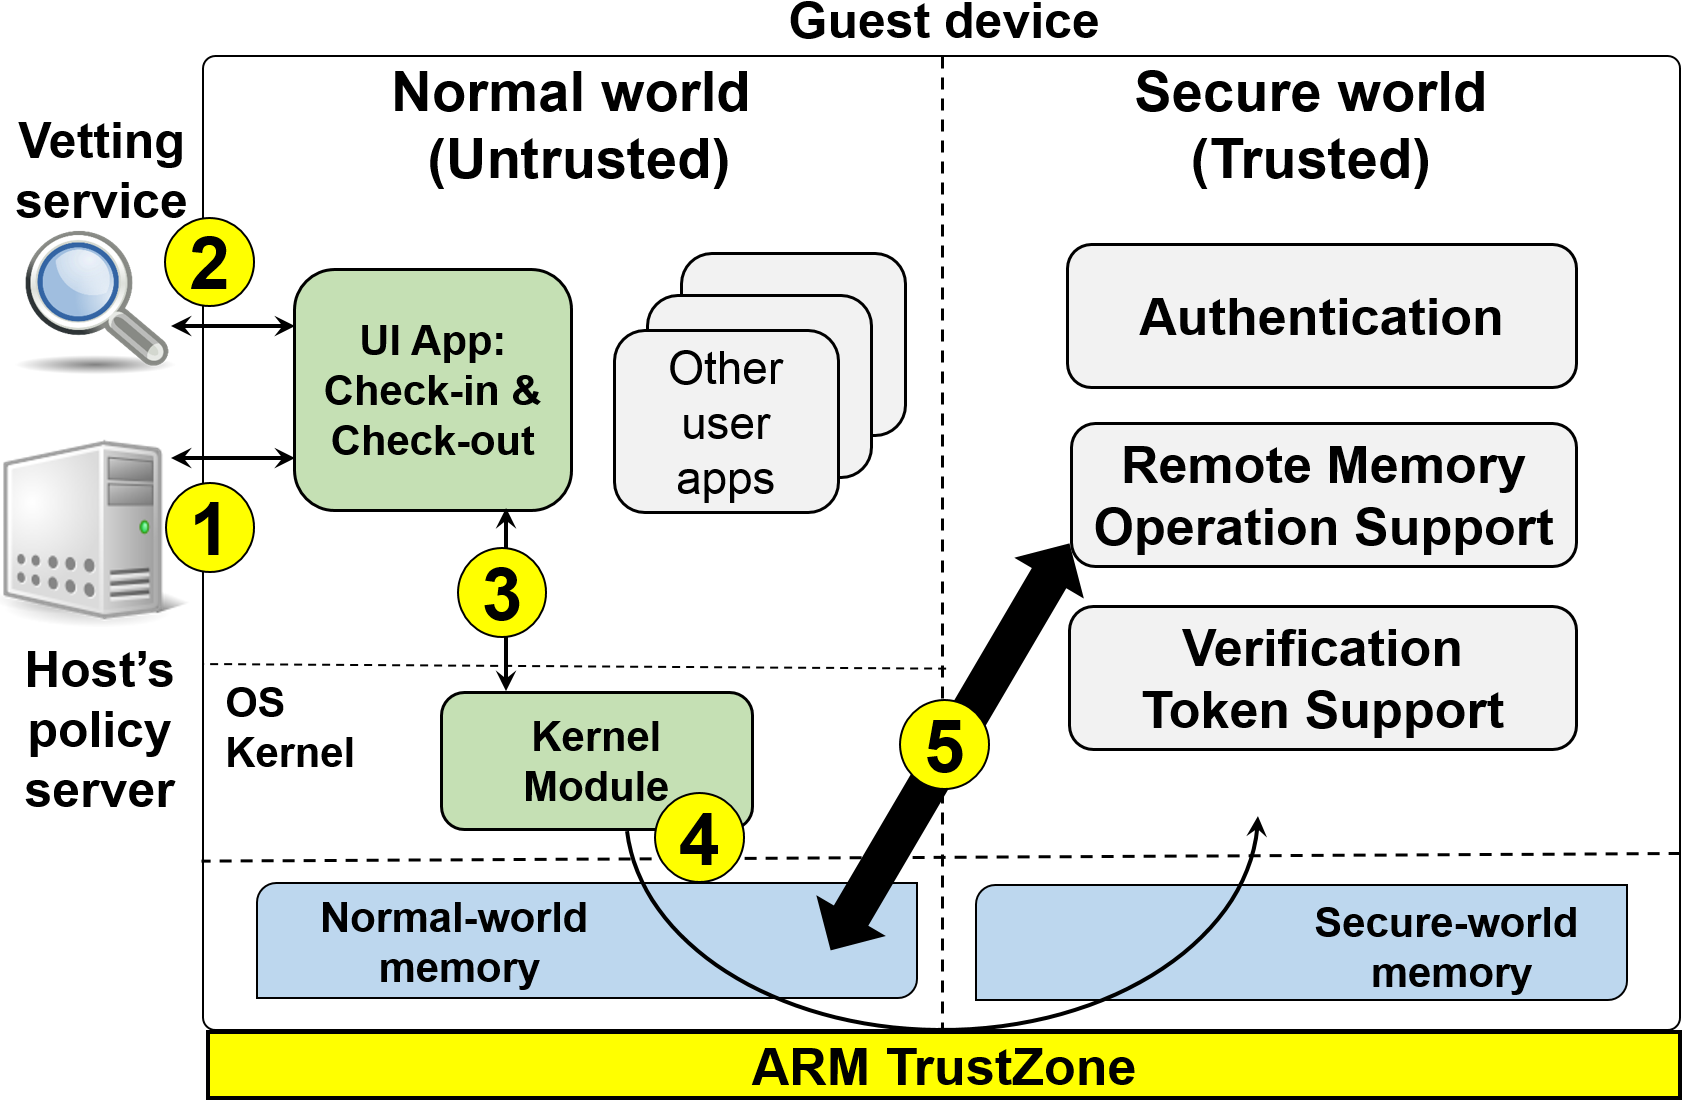
\includegraphics[keepaspectratio=true,width=0.45\textwidth]{figures/overall-design.png}
%\indent\vspace{-0.1cm}
\mycaption{Guest device setup showing components of the policy enforcement
mechanism. (1)~The host communicates with the UI app on the guest and sends
requests to perform remote memory operations. (2)~The UI app uses the vetting
service to determine the safety of the request. (3)~If determined to be safe,
the UI app forwards this request to the supporting kernel module. (4)~The
kernel module invokes the secure world by performing a world switch. (5)~The
secure world performs the requested memory operations on the normal world
memory on behalf of the host.  The components in the normal world, \ie~the UI
app and the kernel module are untrusted. The TCB consists of only the
components that execute in the secure world.}{\label{figure:overall}}
%\indent\vspace{-0.3cm}
\end{figure}

Guest devices are therefore set up as shown in \figref{figure:overall}.  Within
the normal world, the end-user interacts with the host as well as with the
secure world via a user-level app (called the UI app).  This app serves as the
end-user's interface to the host, allowing him to perform operations such as
check-in and check-out of the device. The app interacts with the components in
the secure world via a kernel module. The host sends a request to perform
remote memory operations on the guest device to the app. The app determines the
safety of this request using the vetting service (\sectref{section:vetting}),
and forwards the request to the kernel module, which invokes \texttt{smc} to
world switch into secure world. The components of the secure world then perform
the request and communicate any return values to the host via the UI app. 

We do not place any restrictions on how the host communicates with the guest.
Thus, the host's policy server could be hosted on the cloud and communicate
with the guest device over WiFi or 3G. Alternatively, the host could install
physical scanners at a kiosk or on the entryway to the restricted space.  The
guest devices would use Bluetooth, NFC, or their USB interface to pair with the
scanner and use it to communicate with the host.

One of the key features of our approach is that the core mechanisms that run
on the TCB in the guest device are \textit{platform-agnostic} and
\textit{policy-agnostic}.  Rather, they present a narrow read/write interface
that hosts can suitably use to enforce policy. All the complex tasks of device
analysis and deciding policy are shifted to the host. Thus, in principle, we
can use the same TCB mechanisms on guest devices that run Android, iOS and
Windows. Hosts would have separate modules to analyze and control each kind of
guest platform.

\subsection{Authentication}
\label{section:mechanism:auth}
\newcommand{\ks}{$k_s$}
\newcommand{\pub}[1]{{\sf Pub#1}}
\newcommand{\prv}[1]{{\sf Prv#1}}
\newcommand{\enc}[2]{\textsf{Enc}$_{#1}$(#2)}
\newcommand{\cert}[1]{\textsf{Cert}(#1)}

Before accepting any remote memory requests, the guest and the host mutually
authenticate each other. We assume that both the host and the guest device have
public/private key pairs with digital certificates issued by a certifying
authority. The guest device stores its private key \prv{G} in its secure world,
thereby protecting it from the untrusted normal world. 

\begin{figure}[t!]
\footnotesize
\centering
\begin{tabular}{|rll|}
\hline
\multicolumn{3}{|l|}{Let host's public/private keypair be \pub{H},~\prv{H}.}\\
\multicolumn{3}{|l|}{Let guest's public/private keypair be \pub{G},~\prv{G}.}\\
1. & \textbf{Guest} $\rightarrow$ \textbf{Host}:
   & \pub{G}, \cert{\pub{G}}\\
%
2. & \textbf{Host} $\rightarrow$ \textbf{Guest}:
   & \pub{H}, \cert{\pub{H}}\\
%
3. & \multicolumn{2}{p{0.42\textwidth}|}{Guest and host verify
       \cert{\pub{H}} and \cert{\pub{G}}}\\
%
4. & \textbf{Host} $\rightarrow$ \textbf{Guest}:
   & $M$, \enc{\prv{H}}{$M$} (\ie~host signs $M$),\\
%
   & \multicolumn{2}{p{0.42\textwidth}|}{where $M$ is 
	      \enc{\pub{G}}{\ks, timestamp}}\\
%
5. & \multicolumn{2}{p{0.42\textwidth}|}{Guest verifies host's digital 
        signature, decrypts M to obtain \ks, and checks timestamp}\\
%
\hline
\end{tabular}
%\indent\vspace{-0.3cm}
\mycaption{Mutual authentication and establishment of \ks.}
{\label{figure:authentication}}
%\indent\vspace{-0.3cm}
\end{figure}

Authentication is akin to TLS handshakes (\figref{figure:authentication}). The
host and the guest exchange public keys and validate the certificates of these
keys with the issuing authority. The host then computes a session key \ks,
which is then transmitted to the client over an secure channel. Note that \ks\
is only used to protect the integrity of messages transmitted between the guest
and the host and not its secrecy.  The key \ks\ is stored in secure world
memory, and is invisible to the normal world. If the guest is rebooted, \ks\ is
erased from memory.

\subsection{Remote Memory Operations}
\label{section:mechanism:rmo}

\myparagraph{Remote Reads} 
%
The host inspects and modifies the guest device's configuration via remote
memory operations. During check-in the host typically requests the guest to
send raw memory pages from the normal world for analysis.  The UI app receives
this request and performs a world switch to complete the request.  The world
switch suspends the UI app and transfers control to the secure world.  Each
request is a set of virtual memory addresses of pages that must be sent to the
host.   The host also includes a message-authentication code (a SHA1-based HMAC
in our case) with the request. The HMAC is over the body of the request using
the key \ks\ negotiated during the authentication phase.

The secure world checks the integrity of the request using the HMAC. This step
is necessary to ensure that the request was not maliciously modified by the
untrusted components in the normal world. The secure world then translates each
virtual page address in the request to a physical page address by consulting
the page table in the normal world kernel. In this case, the page table will
correspond to the suspended context in the normal world, \ie~that of the UI
app, into which the running kernel is also mapped.  It then creates a
local copy of the contents of this physical page from the normal world, and
computes an HMAC over the page (again using \ks). The page and its HMAC are
then copied to a buffer in the normal world, from where they can be transmitted
to the host by the UI app.  The host checks the HMAC and uses the page for
analysis. This process is iterative, with the host requesting more pages from
the guest based upon the results of the analysis.

Note that in our case, both the host and the secure world are isolated from the
normal world, which is untrusted. We only rely on the normal world kernel to
facilitate communication between the host and the secure world. Moreover, both
the host and the secure world use HMACs to protect the integrity of messages
transmitted via the normal world.  The normal world may drop messages and cause
a denial-of-service attack; however, such attacks are outside our threat model
(see \sectref{section:threat}). The host can therefore reliably obtain the
memory pages of the normal world to enable the kinds of analyses described in
\sectref{section:policy:analysis}. Communication between the host and the
secure world is not confidential and is therefore not encrypted.\footnote{The
host and guest could communicate over TLS, but the TLS channel on the guest
ends at the UI app, which runs in the normal world.} Thus, a malicious normal
world kernel can potentially snoop on the requests from the host to fetch pages
and attempt to remove the infection to avoid detection. However, this would
have the desirable side-effect of cleaning the guest device at check-in.

\myparagraph{Remote Writes}
%
The host reconfigures the guest by modifying the running state of the normal
world kernel via remote write requests. Each write request is a set of triples
$\langle$\textit{vaddr}$_i$,~\textit{val}$_i$,~\textit{old-val}$_i$$\rangle$
together with an HMAC of this request. The normal world conveys this request to
the secure world, which verifies the integrity of the message using its HMAC.
For each virtual address \textit{vaddr}$_i$ (which refers to a memory location
in the virtual address space of the UI app) in the request, the secure world
ensures that the current value at the address matches \textit{old-val}$_i$.  If
all the values match, then the secure world replaces their values with
\textit{val}$_i$. 

Note that because the normal world is frozen during the course of this
operation, the entire update is atomic with respect to the normal world. When
a remote write operation succeeds, the secure world computes and returns a
verification token to the host. If not, it returns an error code denoting a
failure.

A remote write request can fail if the value stored at the virtual address
\textit{vaddr}$_i$ does not match the value \textit{old-val}$_i$.  This problem
arises in our design because the host's remote read and write operations do not
happen as an atomic unit. The host remotely reads pages copied from the normal
world's memory, analyzes them and creates remote write request using this
analysis. During this time, the normal world kernel continues to execute, and
may have updated the value at the address \textit{vaddr}$_i$.

If a remote write operation fails, the host repeats the operation until it
succeeds. That is, it refetches pages from the guest, analyzes them, and
creates a fresh write request. In theory, it is possible that the host's write
requests will fail \textit{ad infinitum}. However, for the setting that we
consider, write operation failures are rare in practice. This is because our
write operations modify the addresses of peripheral device driver hooks.
Operating systems typically do not change the values of device driver hooks
after they have been initialized at system boot. 

In theory, a remote write request can also fail if the virtual address
\textit{vaddr}$_i$ referenced in the request is not mapped to a physical page
in memory, \ie~if the corresponding page has been swapped out to persistent
storage. In practice, however, we restrict remote writes to kernel data pages
that are resident in physical memory, as is the case with device drivers and
pages that store data structures of peripherals. Therefore, we do not observe
failures due to a failure to resolve \textit{vaddr}$_i$s.

It is possible to completely avoid such problems by design if we complete both
the read and write operations in a single world switch. During this time, the
normal world remains frozen and cannot change the view of memory exported to
the host.  The read and write operations will therefore happen as an atomic
unit from the normal world's perspective. However, in this case, the secure
world must have the ability to directly communicate with the host. As already
discussed in \sectref{section:mechanism:overall}, we decided against this
design because it has the unfortunate consequence of bloating the size of the
TCB.  Thus, we make the practical design tradeoff of minimizing the
functionality of the TCB while allowing the rare remote write failure to
happen.

\subsection{Verification Tokens}
\label{section:mechanism:tokens}

The host receives a verification token from the secure world upon successful
completion of a remote write operation. A verification token \textsf{VTok}[$r$]
is the value
%
%\begin{center}
%
$
r||\textit{MemState}||\textsf{HMAC}_{k_s}[r||\textit{MemState}]$
%
%\end{center}
%
where \textit{MemState} is
$\langle\textit{vaddr}_1,~\textit{val}_1\rangle||\ldots||\langle\textit{vaddr}_n,~\textit{val}_n\rangle$,
the set of \textit{vaddr}$_i$ modified by the remote write, and the new values
\textit{val}$_i$ at these locations. The token \textsf{VTok}[$r$] is
parameterized by a random nonce $r$. This nonce can either be provided by the
host together with the remote write request, or can be generated by the secure
world. 

Verification tokens allow the host to determine whether the guest attempted to
revert the configuration changes made by the remote write, either maliciously
or by turning off the guest device. To do so, the host obtains a verification
token \textsf{VTok}[$r_{{\it checkin}}$] upon completion of checkin, and
stores this token for validation. During checkout, the host requests a
validation token \textsf{VTok}[$r_{\it checkout}$] from the guest over the
same virtual memory addresses. The secure world accesses each of these memory
addresses and computes the verification token with $r_{\it checkout}$ as the
nonce. The host can compare the verification tokens
\textsf{VTok}[$r_{{\it checkin}}$] and
\textsf{VTok}[$r_{{\it checkout}}$] to determine whether there were any
changes to the values stored at these memory addresses. 

The nonces $r_{\it checkin}$ and $r_{\it checkout}$ ensure the freshness of the
tokens \textsf{VTok}[$r_{{\it checkin}}$] and \textsf{VTok}[$r_{{\it
checkout}}$].  The use of \ks\ to compute the HMAC in the verification token
ensures that the token is only valid for a specific device and for the duration
of the session, \ie~until check-out or until the device is powered off,
whichever comes earlier. Because \ks\ is only stored in secure world memory, it
is ephemeral and unreadable to the normal world. This ensures that any attempts
to undo the configuration changes performed at check-in will be detected by the
host.

% \subsection{Security Analysis}
% What if kernel module is loaded dynamically? We disable that.



\mysection{Policy Enforcement}
\label{section:mechanism}

We now present the design of our policy enforcement mechanism, which executes
in the guest's secure world. The host must establish a channel to communicate
with the guest's secure world. This channel must be integrity-protected from
adversaries, including the guest's untrusted normal world.  One way to set up
such a channel is to configure the secure world to exclusively control a
communications peripheral, say WiFi, and connect to the host without involving
the normal world. Thus, the secure world must also execute the code necessary
to support this peripheral. For peripherals such as WiFi, this would require
several thousand lines of code from the networking stack to run in the secure
work.

Our design aims to minimize the functionality that is implemented in the secure
world.  In our design, the normal world is assigned all peripherals on the
guest device and therefore controls all external communication from the device.
It establishes the communication channel between the secure world and the host.
All messages transmitted on the channel are integrity-protected by the message
sender using cryptographic checksums. The secure world itself provides support
for just four key operations:
%
mutual authentication (\sectref{section:mechanism:auth}), 
%
remote memory operations (\sectref{section:mechanism:rmo}),
%
verification tokens (\sectref{section:mechanism:tokens}), and
%
REM-suspend (\sectref{section:mechanism:REMsuspend}).

\begin{figure}[t!]
\begin{center}
\begin{tabular}{|c|}
\hline
\indent\vspace{-0.3cm}\\
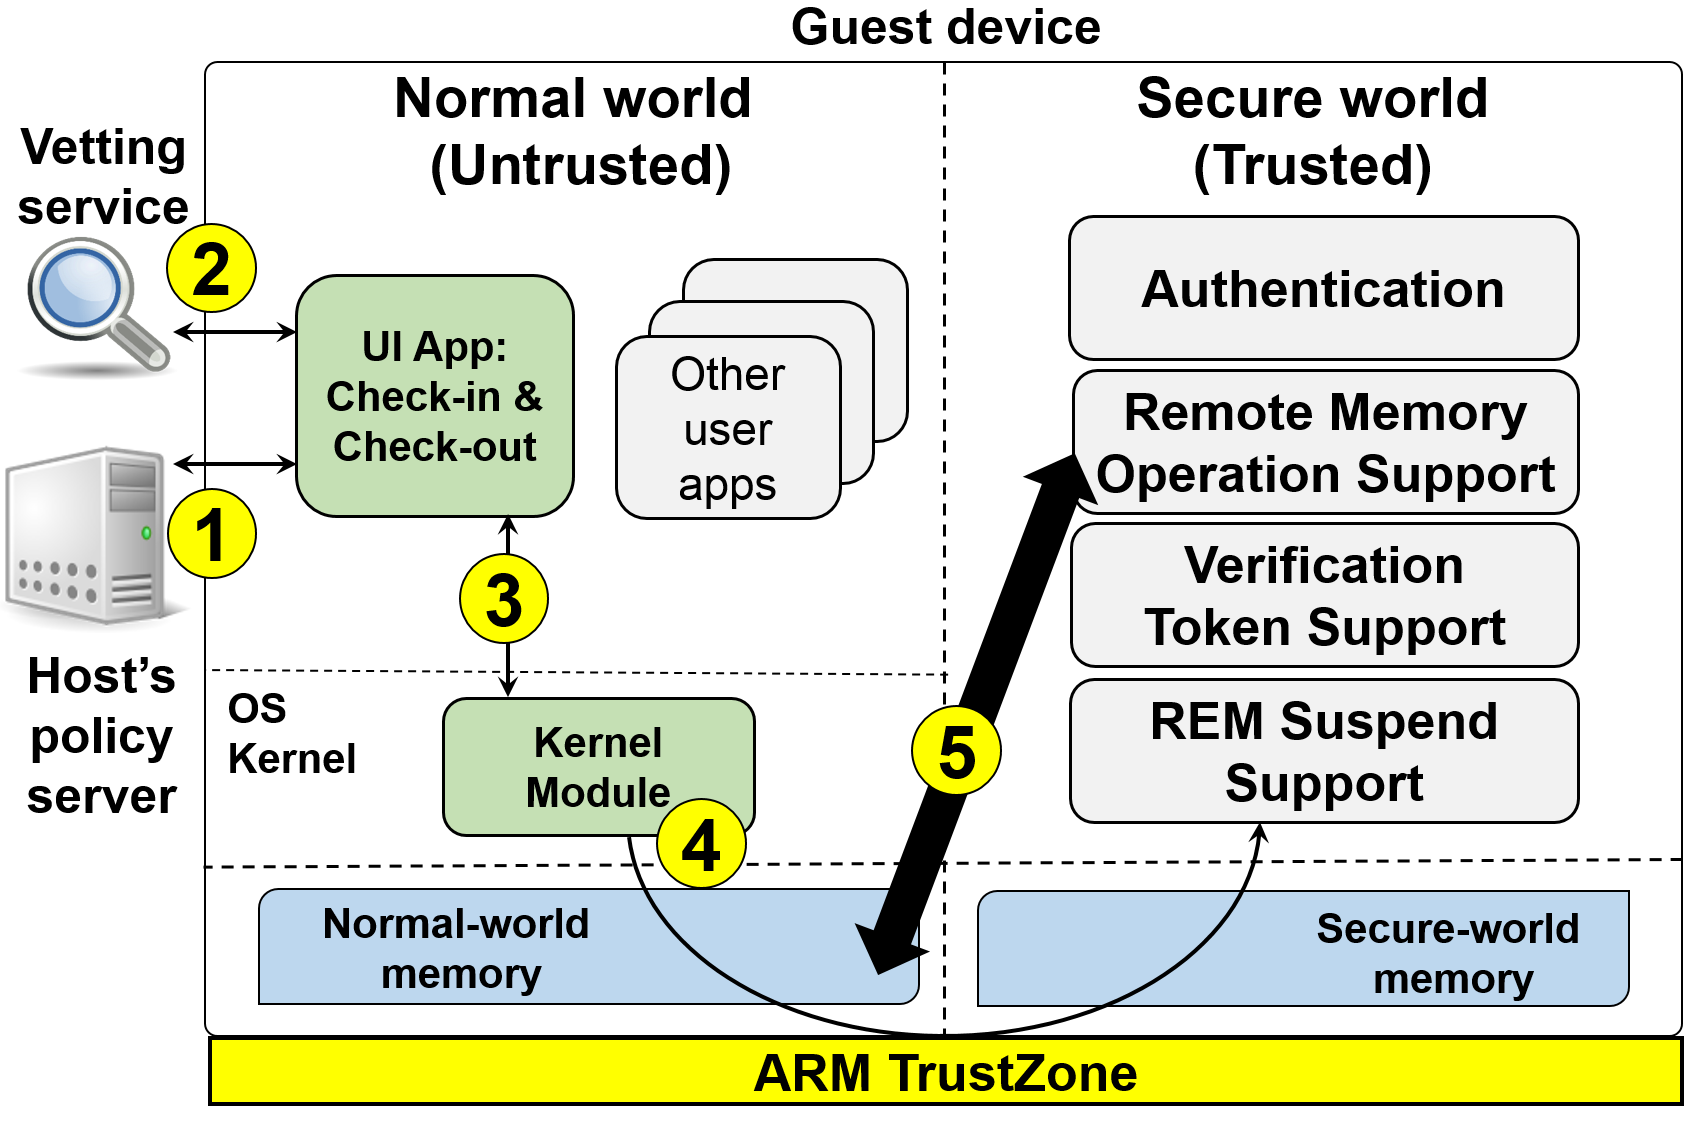
\includegraphics[keepaspectratio=true,width=0.45\textwidth]{overall-design.png}\\
%\indent\vspace{-0.4cm}
\multicolumn{1}{|p{0.47\textwidth}|}
{\small \circone~The host communicates with the UI app on the guest and sends
requests to perform remote memory operations. 
%
\circtwo~The UI app uses the vetting service to determine the safety of the
request. 
%
\circthree~If determined to be safe, the UI app forwards this request to the
supporting kernel module. 
%
\circfour~The kernel module invokes the secure world by performing a world
switch. 
%
\circfive~The secure world performs the requested memory operations on the
normal world memory on behalf of the host.  The components in the normal world
(the UI app and kernel module) are untrusted. We rely on ARM TrustZone's secure
boot to establish trust in the secure world.}\\
\hline
\end{tabular}
\end{center}
\indent\vspace{-0.5cm}
\mycaption{Guest device setup showing components of the policy enforcement
mechanism.}{\label{figure:overall}}
\end{figure}

Guest devices are therefore set up as shown in \figref{figure:overall}.  Within
the normal world, the end-user's interface is a user-level app (called the UI
app) that allows him to interact with the host for device check-in and
check-out. The app interacts with the components in the secure world via a
kernel module. The host sends a request to perform remote memory operations on
the guest device to the app. The app determines the safety of this request
using the vetting service (\sectref{section:vetting}), and forwards the request
to the kernel module, which invokes \textsf{smc} to world switch into secure
world. The components of the secure world then perform the request and
communicate any return values to the host via the UI app. All messages include
a message-authentication code computed using a key established during the
mutual authentication step.

We do not place any restrictions on how the host and guest device communicate.
Thus, the host's policy server could be hosted on the cloud and communicate
with the guest device over WiFi or 3G/4G. Alternatively, the host could install
physical scanners at a kiosk or on the entry-way to the restricted space.  Guest
devices would use Bluetooth, NFC, or USB to pair with the scanner and use it to
communicate with the host.

The core mechanisms that run in the secure world of the guest device have two
key features. They are \textit{policy-agnostic} in that the same mechanisms can
be used to enforce a variety of host policies. The narrow read/write interface
is also \textit{platform-agnostic}, and allows the same mechanisms to work
irrespective of whether the normal world runs Android, iOS or Windows. This
approach shifts complex device analysis and policy formulation tasks to the
hosts. Hosts would naturally need to have separate modules to analyze and
formulate memory updates for various normal world OSes.

\subsection{Authentication}
\label{section:mechanism:auth}
\newcommand{\ks}{$k_s$}
\newcommand{\pub}[1]{{\sf PubKey#1}}
\newcommand{\prv}[1]{{\sf PrivKey#1}}
\newcommand{\enc}[2]{\textsf{Enc}$_{#1}$(#2)}
\newcommand{\cert}[1]{\textsf{Certificate}(#1)}

The host and guest device begin by mutually authenticating each other
(\figref{figure:authentication}). We assume that both the host and the guest
device have public/private key pairs with digital certificates issued by a
certifying authority. The guest device stores its private key \prv{G} in its
secure world, thereby protecting it from the untrusted normal world. 

\begin{figure}[t!]
\footnotesize
\renewcommand{\arraystretch}{0.85}
\centering
\begin{tabular}{|rll|}
\hline
\multicolumn{3}{|l|}{Let host's public/private keypair be \pub{H},~\prv{H}.}\\
\multicolumn{3}{|l|}{Let guest's public/private keypair be \pub{G},~\prv{G}.}\\
1. & \textbf{Guest} $\rightarrow$ \textbf{Host}:
   & \pub{G}, \cert{\pub{G}}\\
%
2. & \textbf{Host} $\rightarrow$ \textbf{Guest}:
   & \pub{H}, \cert{\pub{H}}\\
%
3. & \multicolumn{2}{p{0.42\textwidth}|}{Guest and host verify
       \cert{\pub{H}} and \cert{\pub{G}}}\\
%
4. & \textbf{Host} $\rightarrow$ \textbf{Guest}:
   & $M$, \enc{\prv{H}}{$M$} (\ie~host signs $M$),\\
%
   & \multicolumn{2}{p{0.42\textwidth}|}{where $M$ is 
        \enc{\pub{G}}{\ks, timestamp}}\\
%
5. & \multicolumn{2}{p{0.42\textwidth}|}{Guest verifies host's digital 
        signature, decrypts M to obtain \ks, and checks timestamp}\\
%
\hline
\end{tabular}
\mycaption{Mutual authentication and establishment of \ks.}
{\label{figure:authentication}}
\end{figure}

Authentication is akin to SSL/TLS handshakes. The host and the guest exchange
public keys and validate the certificates of these keys with the issuing
authority. The host then computes a session key \ks, which is then transmitted
to the client over a secure channel. Note that \ks\ is only used to protect
the integrity of messages transmitted between the guest and the host and not
their secrecy. The key \ks\ is stored in secure world memory, and is invisible
to the normal world. It persists across REM-suspends of the guest device, but 
is erased from memory if the device is rebooted.

\addtext{Task 8}{
As with SSL/TLS, the ability of this protocol to resist man-in-the-middle
attacks depends on the host and guest device's ability to validate each other's
public keys. We assume that device vendors would provision \pub{G} for
individual devices and register them with a certifying authority. Hosts
register \pub{H} in much the same manner as is done for Web services today.
While there is a case to be made that the certifying authority model has its
limitations in the era of the Web and smart devices~\cite{sokssl:oak13}, we
note that our use of authentication is entirely standard---to validate the
host's and guest device's identities and to establish a session key \ks.  Thus,
we think that the other parts of our policy enforcement mechanism will work
as-is with alternative authentication schemes, \eg~those that use
identity-based encryption.
}


\subsection{Remote Reads and Writes}
\label{section:mechanism:rmo}

\myparagraph{Remote Reads} 
%
During check-in the host typically requests the guest to send raw memory pages
from the normal world for analysis.  The UI app receives this request and
performs a world switch to complete the request.  The world switch suspends the
UI app and transfers control to the secure world.  Each request is a set (or
range) of virtual memory addresses of pages that must be sent to the host.  The
host also includes a message-authentication code, a SHA1-based HMAC in our
case, with the request. The HMAC is computed on the body of the request using
the key \ks\ negotiated during authentication.

The secure world checks the integrity of the request using the HMAC. This step
is necessary to ensure that the request was not maliciously modified by the
untrusted components in the normal world. The secure world then translates each
virtual page address in the request to a physical page address by consulting
the page table in the normal world kernel. In this case, the page table will
correspond to the suspended context in the normal world, \ie~that of the UI
app, into which the running kernel is also mapped.  It then creates a local
copy of the contents of this physical page from the normal world, and computes
an HMAC over the page (again using \ks). The page and its HMAC are then copied
to a buffer in the normal world, from where they can be transmitted to the host
by the UI app.  The host checks the HMAC and uses the page for analysis. This
process could be iterative, with the host requesting more pages from the guest
device based upon the results of the analysis of the memory pages received up
to that point.

Both the host and the secure world are isolated from the normal world, which is
untrusted. We only rely on the normal world kernel to facilitate communication
between the host and the secure world. Moreover, both the host and the secure
world use HMACs to protect the integrity of messages transmitted via the normal
world.  The normal world may drop messages and cause a denial-of-service
attack; however, such attacks are outside our threat model (see
\sectref{section:threat}). The host can therefore reliably obtain the memory
pages of the normal world to enable the kinds of analyses described in
\sectref{section:policy}. Communication between the host and the secure world
is not confidential and is therefore not encrypted.\footnote{The host and guest
could communicate over SSL/TLS, but this channel on the guest ends at the UI
app, which runs in the normal world.} Thus, a malicious normal world kernel can
potentially snoop on the requests from the host to fetch pages and attempt to
remove the infection to avoid detection. However, this would have the desirable
side-effect of cleaning the guest device at check-in.

\myparagraph{Remote Writes}
%
The host reconfigures the guest by modifying the running state of the normal
world kernel via remote memory updates. The host sends the guest a set of
triples
$\langle$\textit{vaddr}$_i$,~\textit{val}$_i$,~\textit{old-val}$_i$$\rangle$
together with an HMAC of this request. The normal world conveys this message to
the secure world, which verifies its integrity using the HMAC.  For each
virtual address \textit{vaddr}$_i$ (which refers to a memory location in the
virtual address space of the UI app) in the request, the secure world ensures
that the current value at the address matches \textit{old-val}$_i$. If
\textit{all} the \textit{old-val}$_i$ values match, the secure world replaces
their values with \textit{val}$_i$; else the \textit{entire} operation is
aborted.

Because the normal world is frozen during the course of this operation, the
entire update is atomic with respect to the normal world. When a remote write
operation succeeds, the secure world computes and returns a verification token
to the host. If not, it returns an \textsc{Abort} error code denoting failure.

The host's memory update request is aborted if the value stored at
\textit{vaddr}$_i$ does not match \textit{old-val}$_i$.  This design feature is
required because the host's remote read and write operations do not happen as
an atomic unit. The host remotely reads pages copied from the normal world's
memory, analyzes them and creates remote write request using this analysis.
During this time, the normal world kernel continues to execute, and may have
updated the value at the address \textit{vaddr}$_i$.

If the memory update is aborted, the host repeats the operation until it
succeeds. That is, it refetches pages from the guest, analyzes them, and
creates a fresh update. In theory, it is possible that the host's memory
updates will abort \textit{ad infinitum}. However, for the setting that we
consider, aborts are rare in practice. This is because our
write operations modify the addresses of peripheral device driver hooks.
Operating systems typically do not change the values of device driver hooks
after they have been initialized at system boot. 

In theory, a remote memory write can also abort if the virtual address
\textit{vaddr}$_i$ referenced in the request is not mapped to a physical page
in memory, \ie~if the corresponding page has been swapped out to persistent
storage. In practice, however, we restrict remote writes to kernel data pages
that are resident in physical memory, as is the case with device drivers and
pages that store data structures of peripherals. Thus, we do not observe
\textsc{Abort}s due to a failure to resolve \textit{vaddr}$_i$s.

It is possible to completely avoid such problems by designing the both the read
and write operations to complete within a single world switch. During this
time, the normal world remains frozen and cannot change the view of memory
exported to the host. The read and write operations will therefore happen as an
atomic unit from the normal world's perspective. However, in this case, the
secure world must have the ability to directly communicate with the host. As
previously discussed, we decided against this design because it has the
unfortunate consequence of bloating the functionality to be implemented in the
secure world.  Thus, we make the practical design tradeoff of minimizing the
functionality of the secure world while allowing the rare remote write failure
to happen.

\addtext{Task 15}{Note that our approach uses virtual addresses in remote
memory operations. In doing so, we implicitly trust the integrity of page
tables in the normal world kernel, which are used to translate these virtual
addresses to physical ones. Recent work has demonstrated address-translation
redirection (ATRA) attacks that work by maliciously modifying page table
entries and the page table base register~\cite{atra:ccs14}. An ATRA attack
effectively hides malicious code and data modifications by creating shadow
pages containing unmodified code and data, and maliciously modifying page table
entries to redirect requests from a security monitor to these shadow pages.  On
ARM TrustZone devices, it is possible to defend against such attacks by
ensuring that all normal world page table updates are shepherded by the secure
world. This is implemented by modifying the normal world kernel to invoke the
secure world (via \textsf{smc}) for page table updates, and implementing a
suitable security policy within the secure world to ensure the integrity of
these updates~\cite{knox:ccs14,sprobes:most14}. We have not implemented this
defense in our prototype and doing so will require additional code in the
secure world. However, we note that such a defense is already implemented as
part of the secure world in Samsung Knox~\cite{knox:ccs14}. We hypothesize that
a solution that integrates our approach with Knox will therefore be robust
against ATRA attacks.}

\subsection{Verification Tokens}
\label{section:mechanism:tokens}

The host receives a verification token from the secure world upon successful
completion of a remote write operation that updates normal world memory. 
A verification token \textsf{VTok}[$r$] is the following value:
%
%\begin{center}
%
$
r||\textit{MemState}||\textsf{HMAC}_{k_s}[r||\textit{MemState}]$
%
%\end{center}
%
where \textit{MemState} is
$\langle\textit{vaddr}_1,~\textit{val}_1\rangle||\ldots||\langle\textit{vaddr}_n,~\textit{val}_n\rangle$,
the set of \textit{vaddr}$_i$ modified by the remote write, and the new values
\textit{val}$_i$ at these locations. The token \textsf{VTok}[$r$] is
parameterized by a random nonce $r$. This nonce can either be provided by the
host together with the remote write request, or can be generated by the secure
world. 

Verification tokens allow the host to determine whether the guest attempted to
revert the host's memory updates, either maliciously or by turning off the
guest device. To do so, the host obtains a verification token
\textsf{VTok}[$r_{{\it checkin}}$] upon completion of check-in, and stores this
token for validation. During checkout, the host requests a validation token
\textsf{VTok}[$r_{\it checkout}$] from the guest over the same virtual memory
addresses. The secure world accesses each of these memory addresses and
computes the verification token with $r_{\it checkout}$ as the nonce. The host
can compare the verification tokens \textsf{VTok}[$r_{{\it checkin}}$] and
\textsf{VTok}[$r_{{\it checkout}}$] to determine whether there were any changes
to the values stored at these memory addresses. 

The nonces $r_{\it checkin}$ and $r_{\it checkout}$ ensure the freshness of
the tokens
\textsf{VTok}[$r_{{\it checkin}}$] and \textsf{VTok}[$r_{{\it checkout}}$].
The use of \ks\ to compute the HMAC in the verification token ensures that the
token is only valid for a specific device and for the duration of the session,
\ie~until check-out or until the device is powered off, whichever comes
earlier. Because \ks\ is only stored in secure world memory, it is ephemeral
and unreadable to the normal world. Any attempts to undo the host's memory
updates performed at check-in will thus be detected by the host.

% \subsection{Security Analysis}
% What if kernel module is loaded dynamically? We disable that.

\subsection{Restricted Space Mode (REM) Suspend}
\label{section:mechanism:REMsuspend}

\newcommand{\kdev}{{\sf K$_{\sf Dev}$}}
%
If a guest device is rebooted, the host's updates to device memory are undone
and \ks\ is erased from secure world memory, thereby ending the session.
However, it is sometimes necessary to suspend the device in the restricted
space, \eg~to conserve battery power. We design REM-suspend to handle such
cases and allow the session key \ks\ to persist when the device is woken.

The ARM TrustZone allows a device to be configured to route certain interrupts
to the secure world~\cite{armtz}. We route and handle power-button presses and
low-battery events in the secure world by prompting the user to specify whether
to REM-suspend the device. When a guest device is checked into a restricted
space, we configure the default power-down option to be REM-suspend; the
default reverts to the traditional power-down sequence when the device checks
out. The user can consciously choose to bypass REM-suspend, in which case the
device shuts down the traditional way, thus ending the session. The same
happens if the device shuts down due to other causes, \eg~power loss caused by
removing the device's battery. 

When the guest device REM-suspends, the secure world checkpoints normal world
memory, which contains the host's updates, and the key \ks, which are both
restored when the device is woken up. The main challenge is to protect the
confidentiality of \ks. The device user is untrusted, and can read the contents
of persistent storage on the device; \ks\ must thus be stored encrypted with a
key that is not available to the device user.

To achieve this goal, we leverage a feature referenced in the ARM TrustZone
manual~\cite[\S6.3.1]{armtz}, which provisions a device with a
statistically-unique one-time programmable secret key that we will refer to as
\kdev. \kdev\ is located in an on-SoC cryptographic accelerator, and accessible
only to secure world software~\cite[\S6.3.1]{armtz}. \kdev\ cannot be read or
changed outside the secure world, other bus masters or the JTAG~\cite{jtag}.
\kdev\ allows confidential data to be encrypted and bound to the device, and
has previously been referenced in other
research~\cite{tlr:asplos14,sentry:asplos15,ftpm:msrtr,mobiletrustedcomputing:ieee14}.
Note that \kdev\ is not the same as \prv{G}, the device's private key.

In REM-suspend, the secure world first checkpoints normal world memory and CPU
registers, and suspends the execution of the normal world. It sets a bit
\textsf{B$_{\sf REM}$} to record that the device is REM-suspended. It stores
the checkpoint and \textsf{B$_{\sf REM}$}, together with an HMAC of these
values under \ks\ on the device's persistent storage. It also stores to
persistent storage the value of \ks\ encrypted under \kdev.  The untrusted
device user does not know \kdev, and therefore cannot forge the encrypted value
of \ks\ or retrieve the cleartext value of \ks. The HMACs under \ks\ protect
the integrity of the normal world checkpoint and \textsf{B$_{\sf REM}$}.
\addtext{Task 6}{An alternative way to protect the integrity of the normal
world checkpoint and \textsf{B$_{\sf REM}$} is to store them in the
replay-protected memory block (RPMB), a trusted storage partition available on
many mobile devices that come equipped with a embedded multi-media storage
controller. The RPMB offers integrity-protection for stored data, ensures data
freshness by protecting against replay attacks, and has been leveraged in
recent work~\cite{ftpm:msrtr}. However, even with this alternative the
confidentiality of \ks\ needs to be protected by encrypting it using \kdev.}

When the device is woken up, the secure world uses \textsf{B$_{\sf REM}$} to
check if the device is REM-suspended. If so, it uses \kdev\ to retrieve \ks,
verifies the integrity of the normal world checkpoint and \textsf{B$_{\sf
REM}$} using their HMACs, and starts the normal world from this checkpoint.
The device resumes execution under the same session and continues to
produce verification tokens if requested by the host.

\addtext{Task 6}{The original ARM TrustZone manual~\cite{armtz} described
\kdev\ in the context of a hypothetical device, and \kdev\ is not part of the
core specification of the TrustZone architecture. As such, it is not clear how
many deployed devices support \kdev; for example, it is not supported by the
TrustZone-enabled board that we used for our prototype implementation.  Many
emerging ARM TrustZone-based security
solutions~\cite{tlr:asplos14,sentry:asplos15,ftpm:msrtr} rely on the existence
of \kdev, and it is likely that future revisions of the TrustZone architecture
will incorporate such a key. The REM-suspend protocol can be used on any
device that supports \kdev\ or a cryptographic key with similar properties,
\ie~a hardware-provisioned key only accessible from the secure world. 
Note that guest devices that do not support such a key can still be
restricted using our approach. However, the only shortcoming is that without
REM-suspend, a power-down event will undo the memory updates requested by the
host, and clear \ks, thereby terminating the session with the host.}

% \mysection{Guest Privacy and Security}
\label{section:vetting}

We built a vetting service trusted by guests to determine the safety of a
host's request. We built it as a cloud-based server, to which the guest device
forwards the host's memory updates together with a copy of its normal world
memory image (via the UI app). We assume that the device and the vetting
service have authenticated each other as in \figref{figure:authentication} or
use SSL/TLS to obtain a communication channel with end-to-end confidentiality
and integrity guarantees. It may also be possible to implement vetting within
the secure world itself. However, we chose not to do so to avoid bloating the
secure world.

The vetting server checks the host's requests against its safety policies and
returns a \textsc{Safe} or \textsc{Unsafe} response to the device. The response
is bound with a random nonce and an HMAC to the original request in the
standard way to prevent replay attacks. The secure world performs the
operations only if the response is \textsc{Safe}. Guests can configure the
vetting server with domain-specific policies to determine safety.  Our
prototype vetting service, which we built as a plugin to the Hex-Rays IDA
toolkit~\cite{ida-pro}, analyzes memory images and checks for the following
safety policies. Although simple and based on conservative whitelisting, in our
experiments, the policies could prove safety without raising false positives.

\myparagraph{Read-safety} For each request to read from address
\textit{vaddr}$_i$, we return \textsc{Safe} only if \textit{vaddr}$_i$ falls in
a pre-determined range of virtual addresses. In our prototype, acceptable
address ranges only include pages that contain kernel code and kernel data
structures.  The vetting server returns \textsc{Unsafe} if the read request
attempts to fetch any addresses from kernel buffers that store user app data,
or virtual address ranges that lie in app user-space memory.

\myparagraph{Write-safety} Our prototype currently only allows write requests
to \textsc{null}ify peripheral interfaces or install dummy drivers that disable
peripherals. We use the following safety policy for dummy drivers.  For each
function $f$ implemented in the dummy driver, consider its counterpart $f_{\it
orig}$ from the original driver, which the vetting service obtains from the
device's memory image. We return \textsc{Safe} only if the function $f$ is
identical to $f_{\it orig}$, or $f$'s body consists of a single return
statement that returns a \textit{valid} error code (\eg~\textsc{-enomem}). We
define an error code as being valid for $f$ if and only if the same error code
is returned along at least one path in $f_{\it orig}$. The intuition behind
this safety check is that $f$ does not modify the memory state of the device or
introduce new and possibly buggy code, but returns an error code that is
acceptable to the kernel and client user apps.  For more complex dummy drivers
that introduce new code, the vetting service could employ a traditional malware
detector or more complex program analyses to scan this code for safety.


% \begin{figure*}[t!]
\begin{tabular}{cc}
\begin{minipage}{0.34\textwidth}
% \begin{figure}[t!]
\footnotesize
\renewcommand{\arraystretch}{0.45}
\centering
\begin{tabular}{|l|r|}
\hline
\multicolumn{1}{|c|}{\bf Component Name} & \multicolumn{1}{|c|}{\bf LOC}\\
\hline
\hline
\multicolumn{2}{|c|}{\bf \scriptsize Secure World (TCB)}\\
\hline
Memory manager                  & 1,381\\
Authentication                  & 1,285\\
Memory ops. \& verif. tokens    & 305\\
REM-suspend                     & 609\\
\hline
SHA1+HMAC                       & 861\\
X509                            & 877\\
RSA                             & 2,307\\
\hline
\hline
\multicolumn{2}{|c|}{\bf \scriptsize Normal World}\\
\hline
Kernel module                   & 93\\
UI app                          & 72\\
\hline
\end{tabular}
\mycaption{Sizes of components on the guest.}
{\label{table:loc}}
% \end{figure}
\end{minipage} & 
%
\begin{minipage}{0.62\textwidth}
% \begin{figure}[t!]
\footnotesize
\newcommand{\centcol}[1]{\multicolumn{1}{c|}{#1}}
\centering
\renewcommand{\arraystretch}{0.95}
\begin{tabular}{|p{0.78in}|p{0.75in}|p{0.35in}|p{0.5in}|p{0.45in}|p{0.55in}|}
\hline
\textbf{\scriptsize Peripheral uninstalled} 
  & \textbf{\scriptsize Approach used (from \figref{figure:uninstall})} 
  & \textbf{\scriptsize Device used}
  & \textbf{\scriptsize Bytes added or modified} 
	& \textbf{\scriptsize Vetting time (sec.)}
	& \textbf{\scriptsize Verification token (bytes)}\\
\hline
USB (webcam) & \textsc{null}ification  & i.MX53 & \centcol{104} & \centcol{-}    & \centcol{260}\\
USB (webcam) & Dummy driver            & i.MX53 & \centcol{168} & \centcol{2.22} & \centcol{388}\\
Camera       & \textsc{null}ification  & Nexus  & \centcol{140} & \centcol{-}    & \centcol{332}\\
Camera       & Dummy driver            & Nexus  & \centcol{224} & \centcol{2.19} & \centcol{500}\\
WiFi         & Dummy driver            & Nexus  & \centcol{152} & \centcol{5.58} & \centcol{356}\\
3G (Data)    & Dummy driver            & Nexus  & \centcol{192} & \centcol{2.15} & \centcol{436}\\
3G (Voice)   & Dummy driver            & Nexus  & \centcol{124} & \centcol{2.15} & \centcol{300}\\
Microphone   & Dummy driver            & Nexus  & \centcol{164} & \centcol{2.27} & \centcol{380}\\
Bluetooth    & Dummy driver            & Nexus  & \centcol{32}  & \centcol{2.52} & \centcol{116}\\
\hline
\end{tabular}
\mycaption{Peripherals uninstalled using remote write operations to a guest
device.}{\label{table:uninstall}}
% \end{figure}
\end{minipage}
\end{tabular}
\end{figure*}




\begin{figure*}[t!]
\begin{tabular}{cc}
\begin{minipage}{0.34\textwidth}
% \begin{figure}[t!]
\footnotesize
\renewcommand{\arraystretch}{0.45}
\centering
\begin{tabular}{|l|r|}
\hline
\multicolumn{1}{|c|}{\bf Component Name} & \multicolumn{1}{|c|}{\bf LOC}\\
\hline
\hline
\multicolumn{2}{|c|}{\bf \scriptsize Secure World (TCB)}\\
\hline
Memory manager                  & 1,381\\
Authentication                  & 1,285\\
Memory ops. \& verif. tokens    & 305\\
REM-suspend                     & 609\\
\hline
SHA1+HMAC                       & 861\\
X509                            & 877\\
RSA                             & 2,307\\
\hline
\hline
\multicolumn{2}{|c|}{\bf \scriptsize Normal World}\\
\hline
Kernel module                   & 93\\
UI app                          & 72\\
\hline
\end{tabular}
\mycaption{Sizes of components on the guest.}
{\label{table:loc}}
% \end{figure}
\end{minipage} & 
%
\begin{minipage}{0.62\textwidth}
% \begin{figure}[t!]
\footnotesize
\newcommand{\centcol}[1]{\multicolumn{1}{c|}{#1}}
\centering
\renewcommand{\arraystretch}{0.95}
\begin{tabular}{|p{0.78in}|p{0.75in}|p{0.35in}|p{0.5in}|p{0.45in}|p{0.55in}|}
\hline
\textbf{\scriptsize Peripheral uninstalled} 
  & \textbf{\scriptsize Approach used (from \figref{figure:uninstall})} 
  & \textbf{\scriptsize Device used}
  & \textbf{\scriptsize Bytes added or modified} 
	& \textbf{\scriptsize Vetting time (sec.)}
	& \textbf{\scriptsize Verification token (bytes)}\\
\hline
USB (webcam) & \textsc{null}ification  & i.MX53 & \centcol{104} & \centcol{-}    & \centcol{260}\\
USB (webcam) & Dummy driver            & i.MX53 & \centcol{168} & \centcol{2.22} & \centcol{388}\\
Camera       & \textsc{null}ification  & Nexus  & \centcol{140} & \centcol{-}    & \centcol{332}\\
Camera       & Dummy driver            & Nexus  & \centcol{224} & \centcol{2.19} & \centcol{500}\\
WiFi         & Dummy driver            & Nexus  & \centcol{152} & \centcol{5.58} & \centcol{356}\\
3G (Data)    & Dummy driver            & Nexus  & \centcol{192} & \centcol{2.15} & \centcol{436}\\
3G (Voice)   & Dummy driver            & Nexus  & \centcol{124} & \centcol{2.15} & \centcol{300}\\
Microphone   & Dummy driver            & Nexus  & \centcol{164} & \centcol{2.27} & \centcol{380}\\
Bluetooth    & Dummy driver            & Nexus  & \centcol{32}  & \centcol{2.52} & \centcol{116}\\
\hline
\end{tabular}
\mycaption{Peripherals uninstalled using remote write operations to a guest
device.}{\label{table:uninstall}}
% \end{figure}
\end{minipage}
\end{tabular}
\end{figure*}



\mysection{Guest Privacy and Security}
\label{section:vetting}

We built a vetting service trusted by guests to determine the safety of a
host's request. We built it as a cloud-based server, to which the guest device
forwards the host's memory updates together with a copy of its normal world
memory image (via the UI app). We assume that the device and the vetting
service have authenticated each other as in \figref{figure:authentication} or
use SSL/TLS to obtain a communication channel with end-to-end confidentiality
and integrity guarantees. It may also be possible to implement vetting within
the secure world itself. However, we chose not to do so to avoid bloating the
secure world.

The vetting server checks the host's requests against its safety policies and
returns a \textsc{Safe} or \textsc{Unsafe} response to the device. The response
is bound with a random nonce and an HMAC to the original request in the
standard way to prevent replay attacks. The secure world performs the
operations only if the response is \textsc{Safe}. Guests can configure the
vetting server with domain-specific policies to determine safety.  Our
prototype vetting service, which we built as a plugin to the Hex-Rays IDA
toolkit~\cite{ida-pro}, analyzes memory images and checks for the following
safety policies. Although simple and based on conservative whitelisting, in our
experiments, the policies could prove safety without raising false positives.

\begin{mybullet}
%
\item \textsf{\textbf{Read-safety.}} For each request to read from address
\textit{vaddr}$_i$, we return \textsc{Safe} only if \textit{vaddr}$_i$ falls in
a pre-determined range of virtual addresses. In our prototype, acceptable
address ranges only include pages that contain kernel code and kernel data
structures.  The vetting server returns \textsc{Unsafe} if the read request
attempts to fetch any addresses from kernel buffers that store user app data,
or virtual address ranges that lie in app user-space memory.
%
\item \textsf{\textbf{Write-safety.}} Our prototype currently only allows write
requests to \textsc{null}ify peripheral interfaces or install dummy drivers
that disable peripherals. We use the following safety policy for dummy drivers.
For each function $f$ implemented in the dummy driver, consider its counterpart
$f_{\it orig}$ from the original driver, which the vetting service obtains from
the device's memory image. We return \textsc{Safe} only if the function $f$ is
identical to $f_{\it orig}$, or $f$'s body consists of a single return
statement that returns a \textit{valid} error code (\eg~\textsc{-enomem}). We
define an error code as being valid for $f$ if and only if the same error code
is returned along at least one path in $f_{\it orig}$. The intuition behind
this safety check is that $f$ does not modify the memory state of the device or
introduce new and possibly buggy code, but returns an error code that is
acceptable to the kernel and client user apps.  For more complex dummy drivers
that introduce new code, the vetting service could employ a traditional malware
detector or more complex program analyses to scan this code for safety.
%
\end{mybullet}

\addtext{Tasks 3\&12}{We implemented the above safety policies in a 190-line
Python plugin to the IDA toolkit. In the following section, we report the
performance of the vetting server as it established the safety of various host
requests to uninstall guest device peripherals. Although we have only explored
the simple safety policies discussed above, the vetting service can implement
more complex policies, and we plan to experiment with such policies in future
work. For example, although our read-safety policy ensures that only kernel
code and data pages can be sent to the host, even these pages may compromise
the guest's privacy. The buffer cache and various buffers used by the
networking stack reside in kernel data pages, and may store sensitive user
information. A more nuanced read-safety policy would identify which memory
addresses store such data and mark as \textsc{Unsafe} any host requests to
fetch data from those addresses. Note that implementing more complex vetting
policies will increase the code-base of the vetting service, which the guest
trusts. However, this complexity does not affect the size of the TCB running on
the guest device.}


% \begin{table*}
\small
\centering
\begin{tabular}{|l|c|c|c|c|c|c|c|}
\hline
\multicolumn{1}{|c|}{\bf Library} &
  {\bf \scriptsize \#Classes} &
  {\bf \scriptsize \#Methods} &
  {\bf \scriptsize \#Tests} &
  {\bf \scriptsize \#Inconsistencies} & % Data to be supplied by Nader.
  \multicolumn{3}{c|}{\underline{\bf \scriptsize \#Unique bugs (by type)}}\\
& & & & & {\bf \scriptsize Type 1} & {\bf \scriptsize Type 2} & {\bf \scriptsize Type 3}\\
\hline
\hline
\code{Microsoft.CSharp} & 
  6    &   56   &  1,848  &     0 & 0 &  0  & 0\\
\code{Microsoft.VisualBasic} & 
  17   &  127   &    613  &     0 & 0 &  0  & 0\\
\code{System.Collections.Concurrent} & 
  10    &   77   &   349  &     0 & 0 &  0  & 0\\
\code{System.Collections} & 
  29    &  172   &   532  &     0 & 0 &  0  & 0\\
\code{System.ComponentModel} & 
   5    &    4   & 1,578  &     0 &  0 &  0  & 0\\
\code{System.Dynamic.Runtime} & 
  29   &   201   &   790  &     4 &  1 &  0  & 0\\
\code{System.Globalization} & 
  14   &   288   &   567  &    29 &  3 &  3  & 0\\
\code{System.Linq} & 
  5    &   172   &   591  &     0 &  0 &  0  & 0\\
\code{System.Linq.Expressions} & 
  44   &   633   &   590  &     6 &  1 &  0  & 1\\
% \code{System.Linq.Parallel} & 
%  6   &   195  & ??    &  X & 0 &  0  & 0\\
\code{System.Net.Http} & 
  44   &   524   &   746  &    21 &  3 &  0  & 3\\
\code{System.Net.NetworkInformation} & 
  1   &      1   &     1  &     0 &  0 &  0  & 0\\
\code{System.Net.Primitives} & 
  13   &   105   &   956  &    30 &  0 &  1  & 1\\
\code{System.Net.Requests} & 
  10    &  122   & 1,269  &     0 &  0 &  0  & 0\\
\code{System.ObjectModel} & 
  16   &    52   & 1,573  &     0 &  0 &  0  & 0\\
\code{System.Reosurces.ResourceManager} & 
  4    &    28   & 1,333  &    46 &  0 &  1  & 0 \\
\code{System.Runtime.Extensions} & 
  12   &   409   &  946   &    28 &  3 &  1  & 1\\
\code{System.Runtime.Numerics} & 
   2   &   170   & 1,514  &    35 &  3 &  0  & 2\\
\code{System.Runtime.Serialization.Json} & 
   4   &    37   & 1,642  &   940 &  1 &  0  & 0\\
\code{System.Runtime.Serialization.Primitives} & 
  13   &    86   & 1,387  &     5 &  1 &  0  & 1\\
\code{System.Runtime.Serialization.Xml} & 
  14   &   342   &  420   &    63 &  1 &  3  & 1\\
\code{System.Text.Encoding} & 
   5   &    66   &  940   &     5 &  1 &  0  & 0\\
\code{System.Text.RegularExpressions} & 
  10   &   103   &  848   &     0 &  0 &  0  & 0\\
\code{System.Xml.ReaderWriter} & 
  24   &   346   &  820   &    51 &  2 &  3  & 3\\
\code{System.Xml.XDocument} & 
  23   &   637   &  612   &    47 &  0 &  1  & 1\\
\hline
\hline
\multicolumn{1}{|c|}{\bf Total} &
  {\bf 354}   & % {\bf 360} &
  {\bf 4,758} & % {\bf 4,953} &
  {\bf 22,465} &
  {\bf 1,310} &
  \multicolumn{3}{c|}{\bf 47}\\
\hline
\end{tabular}
\mycaption{Summary of inconsistencies found by \tool\ in various Xamarin
libraries. This table shows the number of classes in each library and the
number of methods in these classes. It also shows the number of test cases that
\tool\ generated for those libraries, the total number of inconsistencies
reported by these test cases, and the number of unique causes for these
inconsistencies. These inconsistencies are sorted by type, as defined in
\tabref{table:inconsistency-sources}.}{\label{table:xcheckresults}}
\end{table*}

\section{Experimental Results}
\label{section:evaluation}

\myparagraph{Setup}
%
For our experimental evaluation, we used Xamarin.Android version 4.16.0,
business edition. We chose Windows 8.1 as the home platform, and Android 4.0.3
(API level 15) as the target platform. As discussed in
\sectref{section:implementation}, we generate test cases on a desktop version
of Windows, and then run these cases on Windows Phone and Android platforms.
Both the phone and desktop version of Windows use \code{.NET} version
4.5.51641. We use Visual Studio Ultimate 2013 version 12.0.30501 as the IDE to
compile our test cases. This environment supports a package that integrates the
tools for Windows Phone 8.1 into the controls of Visual Studio. We also use the
same development environment to build the Android version using Xamarin. In
particular, we use the Xamarin 3.5.58.0 extension to enable development for
Xamarin.Android within Visual Studio.

We use emulators to mimic Windows Phone and Android devices. Microsoft offers a
few pre-configured emulation environments for Windows Phone: our experiments
use Emulator 8.1/WVGA-4inch/512MB configuration. We configured the Android
emulator to match the hardware configurations of the Windows Phone emulator.
% All experiments on Intel Core-i7-3770 at 3.4GHz, 16GB RAM, Windows 8.1 Pro.

\myparagraph{Inconsistent Behavior}
%
\tabref{table:xcheckresults} presents the results of our experiments.  To date,
we have used \tool\ to generate \checkme{22,465} test cases, which invoke
\checkme{4,758} methods implemented in \checkme{354} classes across
\checkme{24} Xamarin DLLs. In all, we observed \checkme{1,310} instances of
inconsistent behavior, which could be attributed to \checkme{47} unique causes.
The results also show a detailed breakdown of these causes by category, where
the type of the inconsistency is as defined in
\tabref{table:inconsistency-sources}. A large number of these instances
(\checkme{940}) stemmed from a single root cause in the test cases for
\code{System.Runtime.Serialization.Json}.

In most cases, we were quickly able to quickly confirm using MSDN and Xamarin
documentation that the inconsistency was indeed a bug in Xamarin. For each type
of inconsistency in \tabref{table:inconsistency-sources}, the test cases that
induced them and the inconsistent results they produced were largely similar to
the examples described in \sectref{section:example}. However, as described
below, there were a few examples of inconsistencies for which the documentation
was ambiguous. We count these cases also as bugs in
\tabref{table:xcheckresults} because they point to unclear documentation.

\begin{mybullet}
%
\item \textit{Precision in math libraries.} We observed two inconsistencies
that were related to precision with which math libraries used rounding and
precision to represent numbers. In one test case, a call to
\code{System.Math.IEEERemainder(double x, double y)} was invoked with
\code{x}=\code{1.49089193085384E-81} and \code{y}=\code{2.22275874948508E-162}.
The Windows Phone version returns a result of \code{3.33639470813326E-163},
while the Android version produced by Xamarin returns \code{0}. 

The second test case was a method sequence with two calls. The first call,
\code{System.Math.Round}\code{(Decimal d, int i, MidpointRounding mode)} was
invoked in the test case as \code{System.Math.Round(2, 3, ToEven)}. According
to the documentation, this call returns the value \code{d} rounded with
\code{i} fractional digits in the given \code{mode}. The Windows Phone version
returns \code{2.000} while the Android version returns \code{2}. While these
are equivalent if used in a mathematical calculation, the second call in the
test case converted them to strings using \code{System.Convert.ToString}, which
resulted in inconsistent serialized state.
%
\item \textit{Ambiguous exception semantics.} We observed one test case where
different exceptions were raised for the same failing method call because of
ambiguity in the semantics of the exception to be raised.  According to
documentation, the \code{NameTable.Add}\code{(Char[] key, int start, int len)}
call can throw two types of exceptions. It throws
\code{IndexOutOfRangeException} when any one of these three conditions is met:
0$>$\code{start}, \code{start}$\geqslant$\code{key.Length}, or
\code{len}$\geqslant$\code{key.Length}. It throws
\code{ArgumentOutOfRangeException} if \code{len}$<$0.

In one of our test cases, the values of \code{start} and \code{len} were such
that 0$>$\code{start} and \code{len}$<$0. For this test case, both the Windows
Phone and desktop versions threw \code{IndexOutOfRangeException} whereas
Xamarin's Android code threw \code{ArgumentOutOfRangeException}. Although both
implementations are correct, the documentation must be clarified to remove this
ambiguity.
%
\end{mybullet}

\myparagraph{False Positives}
%
As previously mentioned, \tool's test cases can sometimes produce false
positives, \ie~cases where inconsistencies do not indicate bugs in Xamarin.  In
our experiments, we observed a total of \checkme{667} such false positives
(these are in addition to the \checkme{1,310} inconsistencies reported in
\tabref{table:xcheckresults}).  However, we were able to narrow down all such
false positives into two broad categories:
%
\begin{mybullet}
%
\item \textit{Documented deviations of behavior.} For some methods,
documentation specifies that the behavior of the method will vary across
platforms. Thus, the Xamarin and \code{.NET} implementations of these methods
need not be similar. The most prominent such example that we encountered in our
test cases was the \code{Object.GetHashCode} method, which can return different
values based on the platform it is invoked on. Another example was the
constructor for the \code{UriBuilder} class. The documentation specifies that
if this class is implemented in a PCL, then if an invalid URI is provided as
the string argument to the constructor, it must throw a \code{FormatException}
instead of a \code{UriFormatException}.

While the above are examples where the documentation specified behavior
deviations, we also observed cases where the deviations were undocumented, but
known to the developers of the platform. One such example is the method
\code{ReadContentAsString} from the class \code{XmlDictionaryReader}. When
included in a test case, this method showed inconsistent behavior across the
Windows Phone and Android versions. However, when we tried to identify the
cause of this bug by examining the source code of the Mono platform (which
Xamarin extends to provide a cross-platform implementation of \code{.NET}), we
found that it was marked with a \code{MonoTODO} attribute, indicating a known
issue with its implementation.
%
\item \textit{Use of platform-specific features.} Some API methods, such as
those from \code{System.Random} and \code{System.Time}, invoke
platform-specific features and return different values when invoked on
different platforms. For example, the \code{System.Net.Cookie()} constructor
initializes \code{Cookie.TimeStamp} with the current system time. Because our
emulation environments for both platforms are not synchronized, this call will
return different values.

Another source of false positives was because the Mono runtime included in a
Xamarin-produced Android app uses Mono Assemblies as its libraries. These
libraries have different metadata information than their Windows Phone
counterparts, and any calls that access this metadata will result in
inconsistent serialized state.
%
\end{mybullet}

Fortunately, it is relatively easy to filter out such false positives. We
simply ignore the warnings about inconsistent serialized state raised by test
cases invoking methods that either have documented behavior deviations, or
invoke platform-specific features. Thus, with just a few filters to eliminate
the causes above, we were able to eliminate all the false positives from the
warnings emitted by \tool's test cases.

\myparagraph{Performance}
%
Finally, we report the time taken to run test cases on our experimental setup.
We ran the Windows Phone and Android emulators on a desktop system running
Windows 8.1 professional edition, and equipped with an Intel Core-i7-3770
running at 3.4GHz, 16GB of RAM. We created an app that packaged 1000
randomly-generated tests and ran the Windows Phone and Android versions of this
app on both emulators. The Android emulator took 29.1 seconds to run the app,
while the Windows Phone emulator took 2.7 seconds. The Android emulator is much
slower because it emulates the ARM architecture atop our Intel platform. In
contrast, the Windows Phone ``emulator'' uses hyper-V and is implemented as a
virtual machine.


\mysection{Implementation and Evaluation}
\label{section:evaluation}

We implemented our policy enforcement mechanism on a i.MX53 Quick Start Board
from Freescale as our guest device. This board is TrustZone-enabled and has a
1GHz ARM Cortex A8 processor with 1GB DDR3 RAM. We chose this board as the
guest device because it offers open, programmable access to the secure world.
In contrast, the vendors of most commercially-available TrustZone-enabled
devices today lock down the secure world and prevent any modifications to it. A
small part of main memory is reserved for exclusive use by the secure world. On
our i.MX53 board, we assigned the secure world 256MB of memory, although it may
be possible to reduce this with future optimizations. The normal world runs
Android 2.3.4 atop Linux kernel version 2.6.35.3.

We built a bare-metal runtime environment for the secure world, just enough to
support the components shown in \figref{figure:overall}. This environment has a
memory manager, and a handler to parse and process commands received from the
host via the normal world. To implement cryptographic operations, we used
components from an off-the-shelf library called the ARM mbed TLS
(v1.3.9)~\cite{polarssl}.  Excluding the cryptography library, our secure world
consists of about 3,500 lines of C code, including about 250 lines of inline
assembly.  
%
\addtext{Task 6}{The secure world implements all the features described in
\sectref{section:mechanism}, except for one minor deviation in the
implementation of the REM-suspend protocol. The i.MX53 does not support \kdev,
so our prototype implements REM-suspend assuming that such a key is available
and can be fetched from hardware.}

\figref{table:loc} shows the sizes of various components.  We used mbed TLS's
implementation of SHA1 and HMACs, RSA and X509 certificates.  As shown in
\figref{table:loc}, the files implementing these components alone comprise only
about 4,000 lines of code. In addition to these secure world components, we
built the kernel module and the UI app (written as a native daemon) for the
normal world, comprising 165 lines of code.  We implemented a host policy
server that authenticates guest devices, and performs remote memory operations.
We conducted experiments to showcase the utility of remote reads and writes to
enforce the host's policies on the guest. The guest and the host communicate
over WiFi.
%
% Host's policy server: 1756 (plus 48LOC of python for memory analysis). 

\myparagraph{Guest Device Analysis}
%
To illustrate the power of remote memory read operations to perform device
analysis, we wrote a simple rootkit that infects the guest's normal world
kernel by hooking its system call table. In particular, it replaces the entry
for the \textsf{close} system call to instead point to a malicious function
injected into the kernel. The malicious functionality ensures that if the
process invoking \textsf{close} calls it with a magic number, then the process
is elevated to \textsf{root}.  Although simple in its operation, Petroni and
Hicks~\cite{sbcfi:ccs07} show that over 95\% of all rootkits that modify kernel
data operate this way.

We were able to detect this rootkit on the host by remotely reading and
analyzing the guest's memory pages. We remotely read pages containing the
\textsf{init}, \textsf{text} and \textsf{data} sections of kernel memory. Our
analyzer, a 48 line Python script, reads the addresses in the system call table
from memory, and compares these entries with addresses in \textsf{System.map}.
If the address is not included, \eg~as happens if the entry for the
\textsf{close} system call is modified, it raises an error. For more
sophisticated rootkits that modify arbitrary kernel data structures, the host
can use complex detection algorithms~\cite{sbcfi:ccs07,gib:tdsc11,kop:ccs09}
based on the recursive snapshot traversal method outlined in
\sectref{section:policy}.

For the above experiment, it took the secure world 54 seconds to create an HMAC
over the memory pages that were sent to the host (9.2MB in total). It takes
under a second to copy data from the normal world to the secure world and vice
versa. It may be possible to accelerate the performance of the HMAC
implementation using floating point registers and hardware acceleration, but we
have not done so in our prototype.

% \newcommand{\apperr}{\textsc{\small AppErrMsg}}
\newcommand{\lostconn}{\textsc{\small LostConn}}
\newcommand{\anderr}{\textsc{\small AndroidErrMsg}}
\newcommand{\emptyfile}{\textsc{\small EmptyFile}}
\newcommand{\blnkscrn}{\textsc{\small BlankScreen}}
\newcommand{\im}{\it\bfseries\small}

\begin{figure*}[htbp!]
%\small
\renewcommand{\arraystretch}{0.5}
\begin{center}
%
%\begin{tabular}{|c|p{0.16\textwidth}|p{0.16\textwidth}|p{0.16\textwidth}|p{0.16\textwidth}|p{0.16\textwidth}|}
\begin{tabular}{|c|c|c|c|c|c|}
\hline
{\bf USB} & {\im MobileWebCam} & {\im Camera ZOOM FX} & {\im Retrica} & {\im Candy Camera} & {\im HD Camera Ultra}\\ 
\hline
\textit{Passive}    & \apperr      & \apperr        & \anderr & \apperr      & \anderr\\
\textit{Active}     & \apperr      & \apperr        & \apperr & \apperr      & \apperr\\
\hline
\hline
{\bf Camera} & {\im Camera for Android} & {\im Camera MX} & {\im Camera ZOOM FX} & {\im HD Camera for Android} & {\im HD Camera Ultra} \\
\hline
\textit{Passive}       & \anderr            & \apperr   & \apperr        & \anderr               & \anderr\\
\textit{Active}        & \blnkscrn          & \apperr   & \anderr        & \blnkscrn             & \blnkscrn\\
\hline
\hline
{\bf WiFi} & {\im Spotify} & {\im Play Store} & {\im YouTube} & {\im Chrome Browser} & {\im Facebook}\\
\hline
\textit{Passive} & \lostconn & \lostconn & \lostconn & \lostconn & \lostconn\\
\textit{Active}  & \lostconn & \lostconn & \lostconn & \lostconn & \lostconn\\
\hline
\hline
{\bf 3G (Data)} & {\im Spotify} & {\im Play Store} & {\im YouTube} & {\im Chrome Browser} & {\im Facebook}\\
\hline
\textit{Passive} & \lostconn & \lostconn & \lostconn & \lostconn & \lostconn\\
\textit{Active}  & \lostconn & \lostconn & \lostconn & \lostconn & \lostconn\\
\hline
\hline
{\bf 3G (Voice)} & \multicolumn{5}{c|}{\im Default call application}\\
\hline
\textit{Passive} & \multicolumn{5}{c|}{\apperr: \small Unable to place a call}\\
\textit{Active}  & \multicolumn{5}{c|}{\apperr: \small Unable to place a call}\\
% {\bf 3G (Voice)} & \multicolumn{5}{p{0.8\textwidth}|}{\im Default call application}\\
% \hline
% \textit{Passive} & \multicolumn{5}{p{0.8\textwidth}|}{\apperr: Unable to place a call}\\
% \textit{Active}  & \multicolumn{5}{p{0.8\textwidth}|}{\apperr: Unable to place a call}\\
\hline
\hline
{\bf Microphone} & {\im Audio Recorder} & {\im Easy Voice Recorder} & {\im Smart Voice Recorder} & {\im Sound and Voice Recorder} & {\im Voice Recorder}\\
\hline
\textit{Passive}           & \apperr        & \apperr             & \apperr              & \apperr    & \apperr\\
\textit{Active}            & \emptyfile     & \emptyfile          & \emptyfile           & \emptyfile & \emptyfile\\
\hline
\end{tabular}
\end{center}
%
\begin{center}
\begin{tabular}{p{0.95\textwidth}}
{\footnotesize We use \textit{Passive} to  denote experiments in which the user app
was not running when the peripheral's driver was replaced with a dummy, and the
app was started after this replacement. We use \textit{Active} to denote
experiments in which the peripheral's driver was replaced with a dummy even as
the client app was executing. 
%
\circone~\apperr\ denotes the situation where the user app starts normally, but
an error message box is displayed within the app after it starts up; 
%
\circtwo~\blnkscrn\ denotes a situation where the user app displayed a blank
screen; 
%
\circthree~\lostconn\ denotes a situation where the user app loses network
connection; 
%
\circfour~\emptyfile\ denotes a situation where no error message is displayed,
but the sound file that is created is empty; 
%
\circfive~\anderr\ denotes the situation where the user app fails to start (in
the passive setting) or a running app crashes (in the active setting), and the
Android runtime system displays an error.}\\
% \hline
\end{tabular}
\end{center}
\indent\vspace{-0.5cm}
\mycaption{Results of robustness experiments for user apps.}
{\label{table:robustness}}
%
\end{figure*}


\newcommand{\apperr}{\textsc{\small AppErrMsg}}
\newcommand{\lostconn}{\textsc{\small LostConn}}
\newcommand{\anderr}{\textsc{\small AndroidErrMsg}}
\newcommand{\emptyfile}{\textsc{\small EmptyFile}}
\newcommand{\blnkscrn}{\textsc{\small BlankScreen}}
\newcommand{\im}{\it\bfseries\small}

\begin{figure*}[htbp!]
%\small
\renewcommand{\arraystretch}{0.5}
\begin{center}
%
%\begin{tabular}{|c|p{0.16\textwidth}|p{0.16\textwidth}|p{0.16\textwidth}|p{0.16\textwidth}|p{0.16\textwidth}|}
\begin{tabular}{|c|c|c|c|c|c|}
\hline
{\bf USB} & {\im MobileWebCam} & {\im Camera ZOOM FX} & {\im Retrica} & {\im Candy Camera} & {\im HD Camera Ultra}\\ 
\hline
\textit{Passive}    & \apperr      & \apperr        & \anderr & \apperr      & \anderr\\
\textit{Active}     & \apperr      & \apperr        & \apperr & \apperr      & \apperr\\
\hline
\hline
{\bf Camera} & {\im Camera for Android} & {\im Camera MX} & {\im Camera ZOOM FX} & {\im HD Camera for Android} & {\im HD Camera Ultra} \\
\hline
\textit{Passive}       & \anderr            & \apperr   & \apperr        & \anderr               & \anderr\\
\textit{Active}        & \blnkscrn          & \apperr   & \anderr        & \blnkscrn             & \blnkscrn\\
\hline
\hline
{\bf WiFi} & {\im Spotify} & {\im Play Store} & {\im YouTube} & {\im Chrome Browser} & {\im Facebook}\\
\hline
\textit{Passive} & \lostconn & \lostconn & \lostconn & \lostconn & \lostconn\\
\textit{Active}  & \lostconn & \lostconn & \lostconn & \lostconn & \lostconn\\
\hline
\hline
{\bf 3G (Data)} & {\im Spotify} & {\im Play Store} & {\im YouTube} & {\im Chrome Browser} & {\im Facebook}\\
\hline
\textit{Passive} & \lostconn & \lostconn & \lostconn & \lostconn & \lostconn\\
\textit{Active}  & \lostconn & \lostconn & \lostconn & \lostconn & \lostconn\\
\hline
\hline
{\bf 3G (Voice)} & \multicolumn{5}{c|}{\im Default call application}\\
\hline
\textit{Passive} & \multicolumn{5}{c|}{\apperr: \small Unable to place a call}\\
\textit{Active}  & \multicolumn{5}{c|}{\apperr: \small Unable to place a call}\\
% {\bf 3G (Voice)} & \multicolumn{5}{p{0.8\textwidth}|}{\im Default call application}\\
% \hline
% \textit{Passive} & \multicolumn{5}{p{0.8\textwidth}|}{\apperr: Unable to place a call}\\
% \textit{Active}  & \multicolumn{5}{p{0.8\textwidth}|}{\apperr: Unable to place a call}\\
\hline
\hline
{\bf Microphone} & {\im Audio Recorder} & {\im Easy Voice Recorder} & {\im Smart Voice Recorder} & {\im Sound and Voice Recorder} & {\im Voice Recorder}\\
\hline
\textit{Passive}           & \apperr        & \apperr             & \apperr              & \apperr    & \apperr\\
\textit{Active}            & \emptyfile     & \emptyfile          & \emptyfile           & \emptyfile & \emptyfile\\
\hline
\end{tabular}
\end{center}
%
\begin{center}
\begin{tabular}{p{0.95\textwidth}}
{\footnotesize We use \textit{Passive} to  denote experiments in which the user app
was not running when the peripheral's driver was replaced with a dummy, and the
app was started after this replacement. We use \textit{Active} to denote
experiments in which the peripheral's driver was replaced with a dummy even as
the client app was executing. 
%
\circone~\apperr\ denotes the situation where the user app starts normally, but
an error message box is displayed within the app after it starts up; 
%
\circtwo~\blnkscrn\ denotes a situation where the user app displayed a blank
screen; 
%
\circthree~\lostconn\ denotes a situation where the user app loses network
connection; 
%
\circfour~\emptyfile\ denotes a situation where no error message is displayed,
but the sound file that is created is empty; 
%
\circfive~\anderr\ denotes the situation where the user app fails to start (in
the passive setting) or a running app crashes (in the active setting), and the
Android runtime system displays an error.}\\
% \hline
\end{tabular}
\end{center}
\indent\vspace{-0.5cm}
\mycaption{Results of robustness experiments for user apps.}
{\label{table:robustness}}
%
\end{figure*}


\myparagraph{Guest Device Control}
%
We evaluated the host's ability to dynamically reconfigure a guest device via
remote memory write operations. For this experiment, we attempted to disable a
number of peripherals from the guest device. However, the i.MX53 board only
supports a bare-minimum number of peripherals. As proof-of-concept, we
therefore tested the effectiveness of remote writes on a Samsung Galaxy Nexus
smart phone with a Texas Instruments OMAP 4460 chipset. This chipset has a
1.2GHz dual-core ARM Cortex-A9 processor with 1GB of RAM, and runs Android 4.3
atop Linux kernel version 3.0.72. This device has a rich set of peripherals,
but its chipset comes with TrustZone locked down, \ie~the secure world is not
accessible to third-party programmers.  We therefore performed remote writes by
modifying memory using a kernel module in its (normal world) OS.  Thus, while
remote writes to this device do not enjoy the security properties described in
\sectref{section:mechanism}, they allow us to evaluate the ability to uninstall
a variety of peripherals from a running guest device.

\figref{table:uninstall} shows the set of peripherals that we uninstalled, the
method used to uninstall the peripheral (from \sectref{section:policy}), the
device on which we performed the operation (i.MX53 or Nexus), and the size of
the write operation, \ie~the number of bytes that we had to modify/introduce in
the kernel.  We were able to uninstall the USB on the i.MX53 and the camera on
the phone by \textsc{null}ifying the peripheral interface. For other
peripherals, we introduced dummy drivers designed according to the safety
criterion from \sectref{section:vetting}. We also used dummy drivers for the
USB and the camera to compare the size of the write operations. In this case,
the size of the write includes both the bytes modified in the peripheral
interface and the dummy driver functions. For the 3G interface, we considered
two cases: that of disabling only 3G data and that of only disabling calls. Our
experiment shows it is possible to uninstall peripherals without crashing the
OS by just modifying a few hundred bytes of memory on the running device. 

\addtext{Tasks 1\&3}{For each uninstalled peripheral, \figref{table:uninstall}
shows the time taken by the vetting service to determine the safety of the
write operation (using the policy from \sectref{section:vetting}). Our vetting
service runs on a quad-core Intel i5-4960 CPU running at 3.5Gz, with 16GB of
memory.  \figref{table:uninstall} also shows the size of the verification token
generated by the secure world for the write operation. The size of the
verification token grows linearly with the size of the write operation, but is
just a few hundred bytes in all cases. On the i.MX53, it took the secure world
under 6 milliseconds to generate the verification tokens. This shows that it is
practical for the host to request the guest device to resend the verification
token at periodic intervals during its stay in the restricted space.}

Installing a dummy driver disables the peripheral, but how does it affect the
user app that is using the peripheral? To answer this question, we conducted
two sets of experiments involving a number of client user apps that leverage
the peripherals shown in \figref{table:uninstall}.  In the first set of
experiments, which we call the \textit{passive setting}, we start with a
configuration where the client app is not executing, replace the device driver
of the peripheral with a dummy, and then start the app. In the second set of
experiments, called the \textit{active setting}, we replace the peripheral's
device driver with the dummy as the client app that uses the peripheral is
executing. 

\figref{table:robustness} shows the results of our experiments. For both the
passive and active settings, we observe that in most cases, the user app
displays a suitable error message or changes its behavior by displaying a blank
screen or creating an empty audio file. In some cases, particularly in the
passive setting, the app fails to start when the driver is replaced, and the
Android runtime displays an error that it is unable to start the app.


% \mysection{Related Work and Design Alternatives}
\label{section:related}

\myparagraph{TrustZone Support}
%
A number of projects have used TrustZone to build novel security applications.
TrustDump~\cite{trustdump:esorics14} is a TrustZone-based mechanism to reliably
acquire memory pages from the normal world of a device (Android
LiME~\cite{lime} and similar tools~\cite{dmd,ddms,recoverymode} do so too, but
without the security offered by TrustZone).  While similar in spirit to remote
reads, TrustDump's focus is to be an alternative to virtualized memory
introspection solutions for malware detection. Unlike our work, TrustDump is
not concerned with restricted spaces, authenticating the host, or remotely
configuring guest devices.

Samsung Knox~\cite{knox:ccs14} and \textsc{Sprobes}~\cite{sprobes:most14}
leverage TrustZone to protect the normal world in real-time from kernel-level
rootkits. These projects harden the normal world kernel by making it perform a
world switch when it attempts to perform certain sensitive operations to kernel
data. A reference monitor in the secure world checks these operations, thereby
preventing rootkits. In our work, remote reads allow the host to detect
infected devices, but we do not attempt to provide real-time protection from
malware. Our work can also leverage Knox to enhance the security of the normal
world (\sectref{section:threat}).

TrustZone has also been used to improve the security of user applications.
Microsoft's TLR~\cite{tlr:asplos14} and Nokia's ObC~\cite{obc:asiaccs09} use
TrustZone to provide a secure execution environment for user apps, even in the
presence of a compromised kernel. Other applications include ensuring
trustworthy sensor readings from peripherals~\cite{tenor:mobisys12} and
securing mobile payments~\cite{proxama}.

\myparagraph{Enterprise Security} With the growing ``bring your own device''
(BYOD) trend, a number of projects have developed enterprise security solutions
that enable multiple persona
(\eg~\cite{asm:sec14,flaskdroid:sec13,cells:sosp11}) or enforce mandatory
access control policies on smart devices
(\eg~\cite{deepdroid:ndss15,seandroid:ndss13,flaskdroid:sec13,asm:sec14}).
Prior work has also explored context-based access control and techniques for
restricted space objects to push usage policies onto guest devices
(\eg~\cite{saint:acsac09,Covington2002,conxsense:asiaccs14,worlddriven:ccs14,blindspot:2009,markit:upside14}).

These projects tend to use one of two techniques. One is to require guest
devices to run a software stack enhanced with a policy enforcement mechanism.
For instance, ASM~\cite{asm:sec14} introduces a set of security hooks in
Android, which consult a security policy (installed as an app) that can be used
to create multiple persona on a device. Each persona is customized with a view
of apps and peripherals that it can use. Another approach is to require
virtualized guest devices
\cite{cells:sosp11,cox:hotmobile07,vmwareverizon,kvmarm:asplos14}. In this
approach, a trusted hypervisor on the guest device enforces isolation between
VMs implementing different persona.

The main benefit of these techniques over our work is the greater app-level
control that they provide. For example, they can be used to selectively block
sensitive audio and blur faces by directly applying policies to the
corresponding user apps~\cite{worlddriven:ccs14,ar:sec13}. These techniques
are able to do so because they have a level of semantic visibility into
app-level behavior that is difficult to achieve at the level of raw memory
operations.

On the other hand, our approach enjoys two main benefits over prior work.
First, our approach simplifies the design of the trusted policy-enforcing code
that runs on guest devices to a TCB of just a few thousand lines of code. In
contrast, security-enhanced OSes and virtualized solutions required hundreds of
thousands of lines of trusted policy-enforcement code to execute on guest
devices.  Prior research has investigated ways to reduce the TCB, \eg~by
creating small hypervisors~\cite{nova:eurosys09}. However, the extent to which
such work on small hypervisors applies to smart devices is unclear, given that
any such hypervisor must support a variety of different virtualization modes,
guest quirks, and hardware features on a diverse set of personal devices.

The second benefit of our approach is that it provides security guarantees that
are rooted in trusted hardware. Prior projects have generally trusted guest
devices to correctly implement the host's policies. This trust can easily be
violated by a guest running a maliciously-modified OS or hypervisor.  It is
also not possible for a host to obtain guarantees that the policy was enforced
for the duration of the guest's stay in the restricted space. We leverage the
TrustZone to offer such guarantees using verification tokens and REM-suspend.

\myparagraph{Other Hardware Interfaces}
%
Hardware interfaces for remote memory operations were originally investigated
for the server world to perform remote DMA as a means to bypass the performance
overheads of the TCP/IP stack~\cite{mellanox,infiniband}.  This work has since
been repurposed to perform kernel malware detection~\cite{copilot:sec04} and
remote repair~\cite{backdoor:icac04}. These systems use a PCI-based
co-processor on guests via which the host can remotely transfer and modify
memory pages on the guest.

On personal devices, the closest equivalent to such a hardware interface is the
IEEE 1394 (Firewire), which is available on some laptops. However, it is not
currently available on smaller form-factor devices.  Another possibility is to
use the JTAG interface~\cite{jtag}, which allows read/write access to memory
and CPU registers via a few dedicated pins on the chipset.  However, the JTAG
is primarily used for debugging and is not easily accessible on consumer
devices.  One drawback of repurposing these hardware interfaces is that they
cannot authenticate the credentials of the host that initiates the memory
operation. Moreover, to use these hardware interfaces on guest devices, the
host needs physical access to plug into them.  Thus, these interfaces are best
used when the guest can physically authenticate the host and trust it to be
benign.


% \myparagraph{App Security}
% 
% It is now well-known that many popular apps exfiltrate sensitive user data
% from smart devices~\cite{taintdroid:osdi10}. Moreover, a significant fraction
% of apps (on Android) are over-privileged~\cite{stowaway:ccs11,pscout:ccs12}
% and end-users are poor at understanding the meaning of app
% permissions~\cite{ep:ubicomp12,felt:soups12}.  Such apps can leverage the
% increasing array of sensors on modern smart devices in novel and dangerous
% ways~\cite{soundcomber:ndss11,placeraider:ndss13}. These threats will amplify
% in the future as we see an increasing number of augmented reality apps that
% continuously monitor sensor feeds and extract data from the device's
% environment.

% Some projects have attempted to rectify the situation by offering improved
% app permission models~\cite{howtoask:hotsec12} or modifying the execution
% environment on the device to return ``fake'' sensor data to
% apps~\cite{mockdroid:hotmobile10}. However, such techniques are usually
% ineffective when the device itself is compromised (\eg~via kernel rootkits),
% or if the user unintentionally installs a malicious app.  Our work can
% complement these efforts by allowing hosts to control peripherals below the
% app layer. 

% \myparagraph{Hardening Smart Devices}
% 
% Finally, the research community has addressed techniques to harden the
% software stack of smart devices. Samsung Knox~\cite{knox:ccs14}, as
% previously discussed, provides the ability to detect certain classes of
% kernel-level rootkits in real time.  MOCFI~\cite{mocfi:ndss12} enhances the
% mobile OS by enforcing control-flow integrity properties,
% thereby mitigating the effect of attacks such as buffer overflow-based
% exploits.  Airbag~\cite{airbag:ndss14} employs lightweight virtualization to
% isolate user apps and prevent them from infecting the device's firmware or
% leaking sensitive information. At the app level,
% RetroSkeleton~\cite{retro:mobisys13} rewrites Android apps to improve their
% security on commodity devices. These techniques can help improve the
% resilience of smart devices to attack. Our work allows hosts to remotely
% analyze smart devices via remote memory operations and verify that they are
% free of malware infection.


% \myparagraph{Defending from Malware}
% \myparagraph{Context Awareness}



% * Clear difference from SAMSUNG KNOX.
% * List the things that we don't want to do (because SAMSUNG KNOX is our competition)
%     - Intercept critical operations.
%     - They cannot detect memory overflow errors.
%     - Ours is asynchronous, theirs is synchronous.
%     - No writes/uninstalling devices.
% * KNOX is not enforcing any enterprise security policy. Ours is enforcing specific enterprise policies.
% * KNOX checks the integrity of certain kernel memory pages.
%
% Prior work has developed numerous examples of security primitives that use
% remote memory operations. Examples include memory forensics~\cite{}, kernel
% malware detection~\cite{}, and OS repair~\cite{}.  
% However, the bulk of these techniques have usually been developed for
% server-class systems or personal computers with larger form factors, such as
% desktops, that typically use the x86 architecture and where methods to isolate
% the target from the monitor, \ie~virtualization or co-processors, are readily
% available.
%


\mysection{Related Work and Alternatives}
\label{section:related}

\myparagraph{TrustZone Support}
%
A number of projects have used TrustZone to build novel security applications.
TrustDump~\cite{trustdump:esorics14} is a TrustZone-based mechanism to reliably
acquire memory pages from the normal world of a device (Android
LiME~\cite{lime} and similar acquisition tools~\cite{dmd,ddms,recoverymode} do
so too, but without the security offered by TrustZone).  While similar in
spirit to remote reads, TrustDump's focus is to be an alternative to
virtualized memory introspection solutions for malware detection. Unlike our
work, TrustDump is not concerned with restricted spaces, authenticating the
host, or remotely configuring guest devices.

Samsung Knox~\cite{knox:ccs14} and \textsc{Sprobes}~\cite{sprobes:most14}
leverage TrustZone to protect the normal world in real-time from kernel-level
rootkits. These projects harden the normal world kernel by making it perform a
world switch when it attempts to perform certain sensitive operations to kernel
data. A reference monitor in the secure world checks these operations, thereby
preventing rootkits. In our work, remote reads allow the host to detect
infected devices, but we do not attempt to provide real-time protection from
malware. Our work can also leverage Knox to enhance the security of the normal
world (\sectref{section:threat}).

\addtext{Task 4}{While we have leveraged TrustZone's ability to isolate secure
world memory from the normal world, TrustZone supports additional features that
can be used to explore alternative designs. One such feature is TrustZone's
support for peripheral reassignment between the normal and secure worlds. Using
this feature, a host could require all of a guest device's restricted
peripherals to the trusted secure world during check-in. The secure world
implements the equivalent of dummy drivers that control and therefore restrict
peripherals.}

\addtext{Task 4}{The above design is a viable alternative that we plan to
explore in future work. In our current design, we chose to explore the benefits
and limits of remote memory operations because it allowed us to satisfy our
goal of minimizing the size of the TCB on guest devices. The alternative design
described above would require additional driver code to execute in the secure
world. That said, even this design alternative can leverage some of the ideas
from our current work. For example, peripherals assigned to the secure world
at check-in can be reassigned to the normal world via a device reboot. A
protocol based on REM-suspend can be used to save peripheral assignment state
upon power-down events, and restore the peripheral assignment upon power-up 
in guest devices that support \kdev. }

TrustZone has also been used to improve the security of user applications.
Microsoft's TLR~\cite{tlr:asplos14} and Nokia's ObC~\cite{obc:asiaccs09} use
TrustZone to provide a secure execution environment for user apps, even in the
presence of a compromised kernel. Other applications include ensuring
trustworthy sensor readings from peripherals~\cite{tenor:mobisys12}, securing
mobile payments (\eg~Apple Pay and Samsung Pay), \addtext{Task 9}{mobile data
billing~\cite{billsplit:hotmobile13}, attesting mobile
advertisements~\cite{adattester:mobisys15}, and implementing the TPM-2.0
specification in firmware~\cite{ftpm:msrtr}.}

\myparagraph{Enterprise Security} With the growing ``bring your own device''
(BYOD) trend, a number of research projects and enterprise MDM products
(\eg~\cite{knox:mdm,ms:intune,blackberry:emm}) have developed security
solutions that enable multiple persona
(\eg~\cite{asm:sec14,flaskdroid:sec13,cells:sosp11}) or enforce mandatory
access control policies on smart devices
(\eg~\cite{deepdroid:ndss15,seandroid:ndss13,flaskdroid:sec13,asm:sec14}).
Prior work has also explored context-based access control and techniques for
restricted space objects to push usage policies onto guest devices
(\eg~\cite{saint:acsac09,Covington2002,conxsense:asiaccs14,worlddriven:ccs14,blindspot:2009,markit:upside14}).

These projects tend to use one of two techniques. One is to require guest
devices to run a software stack enhanced with a policy enforcement mechanism.
For instance, ASM~\cite{asm:sec14} introduces a set of security hooks in
Android, which consult a security policy (installed as an app) that can be used
to create multiple persona on a device. Each persona is customized with a view
of apps and peripherals that it can use. Another approach is to require
virtualized guest devices
\cite{cells:sosp11,cox:hotmobile07,vmwareverizon,kvmarm:asplos14}. In this
approach, a trusted hypervisor on the guest device enforces isolation between
virtual machines implementing different persona.

The main benefit of these techniques over our work is the greater app-level
control that they provide. For example, they can be used to selectively block
sensitive audio and blur faces by directly applying policies to the
corresponding user apps~\cite{worlddriven:ccs14,ar:sec13}. These techniques
are able to do so because they have a level of semantic visibility into
app-level behavior that is difficult to achieve at the level of raw memory
operations.

On the other hand, our approach enjoys two main benefits over prior work.
First, our approach simplifies the design of the trusted policy-enforcing code
that runs on guest devices to a TCB of just a few thousand lines of code. In
contrast, security-enhanced OSes and virtualized solutions required hundreds of
thousands of lines of trusted policy-enforcement code to execute on guest
devices.  Prior research has investigated ways to reduce the TCB, \eg~by
creating small hypervisors~\cite{nova:eurosys09}. However, the extent to which
such work on small hypervisors applies to smart devices is unclear, given that
any such hypervisor must support a variety of different virtualization modes,
guest quirks, and hardware features on a diverse set of personal devices.

The second benefit of our approach is that it provides security guarantees that
are rooted in trusted hardware. Prior projects have generally trusted guest
devices to correctly implement the host's policies. This trust can easily be
violated by a guest running a maliciously-modified OS or hypervisor.  It is
also not possible for a host to obtain guarantees that the policy was enforced
for the duration of the guest's stay in the restricted space. We leverage the
TrustZone to offer such guarantees using verification tokens and REM-suspend.

\myparagraph{Other Hardware Interfaces}
%
Hardware interfaces for remote memory operations were originally investigated
for the server world to perform remote DMA as a means to bypass the performance
overheads of the TCP/IP stack~\cite{mellanox,infiniband}.  This work has since
been repurposed to perform kernel malware detection~\cite{copilot:sec04} and
remote repair~\cite{backdoor:icac04}. These systems use a PCI-based
co-processor on guests via which the host can remotely transfer and modify
memory pages on the guest.

On personal devices, the closest equivalent to such a hardware interface is the
IEEE 1394 (Firewire), which is available on some laptops. However, it is not
currently available on smaller form-factor devices.  Another possibility is to
use the JTAG interface~\cite{jtag}, which allows read/write access to memory
and CPU registers via a few dedicated pins on the chipset.  However, the JTAG
is primarily used for debugging and is not easily accessible on consumer
devices.  One drawback of repurposing these hardware interfaces is that they
cannot authenticate the credentials of the host that initiates the memory
operation. Moreover, to use these hardware interfaces on guest devices, the
host needs physical access to plug into them.  Thus, these interfaces are best
used when the guest can physically authenticate the host and trust it to be
benign.


% \myparagraph{App Security}
% 
% It is now well-known that many popular apps exfiltrate sensitive user data
% from smart devices~\cite{taintdroid:osdi10}. Moreover, a significant fraction
% of apps (on Android) are over-privileged~\cite{stowaway:ccs11,pscout:ccs12}
% and end-users are poor at understanding the meaning of app
% permissions~\cite{ep:ubicomp12,felt:soups12}.  Such apps can leverage the
% increasing array of sensors on modern smart devices in novel and dangerous
% ways~\cite{soundcomber:ndss11,placeraider:ndss13}. These threats will amplify
% in the future as we see an increasing number of augmented reality apps that
% continuously monitor sensor feeds and extract data from the device's
% environment.

% Some projects have attempted to rectify the situation by offering improved
% app permission models~\cite{howtoask:hotsec12} or modifying the execution
% environment on the device to return ``fake'' sensor data to
% apps~\cite{mockdroid:hotmobile10}. However, such techniques are usually
% ineffective when the device itself is compromised (\eg~via kernel rootkits),
% or if the user unintentionally installs a malicious app.  Our work can
% complement these efforts by allowing hosts to control peripherals below the
% app layer. 

% \myparagraph{Hardening Smart Devices}
% 
% Finally, the research community has addressed techniques to harden the
% software stack of smart devices. Samsung Knox~\cite{knox:ccs14}, as
% previously discussed, provides the ability to detect certain classes of
% kernel-level rootkits in real time.  MOCFI~\cite{mocfi:ndss12} enhances the
% mobile OS by enforcing control-flow integrity properties,
% thereby mitigating the effect of attacks such as buffer overflow-based
% exploits.  Airbag~\cite{airbag:ndss14} employs lightweight virtualization to
% isolate user apps and prevent them from infecting the device's firmware or
% leaking sensitive information. At the app level,
% RetroSkeleton~\cite{retro:mobisys13} rewrites Android apps to improve their
% security on commodity devices. These techniques can help improve the
% resilience of smart devices to attack. Our work allows hosts to remotely
% analyze smart devices via remote memory operations and verify that they are
% free of malware infection.


% \myparagraph{Defending from Malware}
% \myparagraph{Context Awareness}



% * Clear difference from SAMSUNG KNOX.
% * List the things that we don't want to do (because SAMSUNG KNOX is our competition)
%     - Intercept critical operations.
%     - They cannot detect memory overflow errors.
%     - Ours is asynchronous, theirs is synchronous.
%     - No writes/uninstalling devices.
% * KNOX is not enforcing any enterprise security policy. Ours is enforcing specific enterprise policies.
% * KNOX checks the integrity of certain kernel memory pages.
%
% Prior work has developed numerous examples of security primitives that use
% remote memory operations. Examples include memory forensics~\cite{}, kernel
% malware detection~\cite{}, and OS repair~\cite{}.  
% However, the bulk of these techniques have usually been developed for
% server-class systems or personal computers with larger form factors, such as
% desktops, that typically use the x86 architecture and where methods to isolate
% the target from the monitor, \ie~virtualization or co-processors, are readily
% available.
%

% \section{Conclusions and Future Work}
\label{section:conclusions}

We see this paper as contributing two main conceptual advances. The first is
the notion of restricted spaces. As argued in the paper, the increasing
ubiquity and capability of smart devices has driven society to create such
restricted spaces. To promote the regulated use of smart devices in such
spaces, we need systematic ways to enforce host-defined policies on guest
devices.

The second conceptual contribution of this paper is the design of a mechanism
for hosts to remotely inspect and control guest devices.  We showed that this
can be achieved via a narrow interface that permits two simple operations,
remote memory reads and writes. These operations provide an effective way for
hosts to analyze and configure guest devices in accordance with their policies.
We also showed that with hardware support from the ARM TrustZone, we can
bootstrap the security of remote memory operations.

While we believe that we have demonstrated the technical feasibility of our
design via a prototype implementation and case studies, a number of issues must
be addressed to make it a practical solution. The foremost such concern is
end-user willingness to subject their devices to regulation in restricted
spaces. It is possible that many users would simply choose not to use their
devices within the restricted space than give the host control over their
devices. However, given our increasing reliance on smart devices and the ways
in which they are becoming integral parts of our daily lives, it is unclear
going forward whether such simple ``opt-out'' solutions would even be a
possibility.  For example, opting-out would not be a practical solution for
smart devices integrated with health monitoring and assistive functionality. 

Even if end-users were willing to subject their devices to regulation, it is
unclear to what extent they will trust the host's control over their device.
Again, we feel that this is largely a matter of user-perception. Users already
place implicit trust in app writers and market vendors when they download apps
on their smart devices. Yet, it is now well-known that apps routinely violate
this implicit trust and compromise user privacy by sending sensitive user data
to unauthorized third parties.  

Thus, a practical deployment of our solution would also likely require
supporting trust infrastructure, \eg~analysis tools that can vet the host's
operations or present them to the end-user in a human-readable format for
approval. We plan to explore such user-interaction and user-perception issues
in future work.


\mysection{Concluding Remarks}
\label{section:conclusions}

% To date, restricted space hosts have largely employed \adhoc\ methods to ensure
% that guest devices are policy-compliant. Going forward, it is not clear that
% \adhoc\ methods alone will suffice. From the guest's perspective, simple
% solutions such as opting not to use devices within restricted spaces are also
% not an option, given our increasing reliance on smart devices. 

This paper develops mechanisms that allow hosts to analyze and regulate ARM
TrustZone-based guest devices using remote memory operations.  These mechanisms
can be implemented with only a small amount of trusted code running on guest
devices. The use of the TrustZone allows our approach to provide strong
guarantees of guest policy-compliance to hosts. Our vetting service allows
guests to identify conflicts between their privacy goals and the hosts' usage
policies. 

While this paper demonstrates technical feasibility of our approach, questions
about its adoptability in real-world settings remain to be answered. For
example, we can imagine our solution to be readily applicable in settings such
as federal or corporate offices and examination halls, where restricted spaces
are clearly demarcated and the expectations on guest device usage are clearly
outlined.  Will it be equally palatable in less stringent settings, such as
social gatherings, malls or restaurants? A meaningful answer to this question
will require a study of issues such as user-perception and willingness to allow
their devices to be remotely analyzed and controlled by hosts. We hope to 
investigate these and other issues in follow-on research.


% We see this paper as making two main conceptual advances. The first is the
% notion of restricted spaces. As argued in the paper, the increasing ubiquity
% and capability of smart devices has driven society to create such restricted
% spaces. To promote the regulated use of smart devices in such spaces, we need
% systematic ways to enforce host-defined policies on guest devices.
% 
% The second conceptual contribution of this paper is the design of a mechanism
% for hosts to remotely inspect and control guest devices.  We showed that this
% can be achieved via a narrow interface that permits two simple operations,
% remote memory reads and writes. These operations provide an effective way for
% hosts to analyze and configure guest devices in accordance with their
% policies.  We also showed that with hardware support from the ARM TrustZone,
% we can bootstrap the security of remote memory operations.
%
% Again, we feel that this is largely a matter of user-perception. For example,
% users already place implicit trust in app writers and market vendors when they
% download apps on their smart devices, even though it is well-known that apps
% routinely violate this implicit trust and compromise user privacy by sending
% sensitive user data to unauthorized third parties.  
%
% Thus, a practical deployment of our solution would also likely require
% supporting trust infrastructure, \eg~analysis tools that can vet the host's
% operations or present them to the end-user in a human-readable format for
% approval.


\myparagraph{Acknowledgments} 
%
% \section*{Acknowledgments}
%
We thank the MobiSys reviewers, our shepherd Ardalan Amiri Sani, Trent Jaeger,
Xinyang Ge, Giuseppe Petracca, and Santosh Nagarakatte for their comments on
drafts of this paper. Daeyoung Kim, Vinod Ganapathy and Liviu Iftode were
supported in part by the US National Science Foundation grants CNS-1441724,
CCF-1408803, CNS-1117711, and CNS-0952128.  Ferdinand Brasser, Christopher
Liebchen and Ahmad-Reza Sadeghi were funded by the German Science Foundation
(DFG) as part of project S2 within CRC~1119 \textsc{crossing}, European Union's
Horizon 2020 research and innovation program under grant agreement number
643964 (\textsc{supercloud}), and the Intel Collaborative Research Institute
for Secure Computing. 

%------------------------------------------------------------------------------
%                                  References.
%------------------------------------------------------------------------------
% \fontsize{9pt}{9pt}
% \selectfont

\small
\renewcommand{\baselinestretch}{1}
\let\oldthebibliography=\thebibliography
  \let\endoldthebibliography=\endthebibliography
  \renewenvironment{thebibliography}[1]{%
    \begin{oldthebibliography}{#1}%
      \setlength{\parskip}{0.25ex}%
      \setlength{\itemsep}{0.25ex}%
  }%
  {%
    \end{oldthebibliography}%
  }

% \bibliographystyle{plain}
% \bibliography{references}

\raggedright
\begin{thebibliography}{10}

\bibitem{ida-pro}
Hex-rays software: About {IDA}.
\newblock \url{https://www.hex-rays.com/products/ida/index.shtml}.

\bibitem{polarssl}
{SSL Library} {ARM} mbed {TLS}/{PolarSSL}.
\newblock \url{https://tls.mbed.org}.

\bibitem{armtz}
{ARM} security technology -- {Building} a secure system using {TrustZone}
  technology, 2009.
\newblock {ARM} Technical Whitepaper.
  \url{http://infocenter.arm.com/help/topic/com.arm.doc.prd29-genc-009492c/PRD%
29-GENC-009492C_trustzone_security_whitepaper.pdf}.

\bibitem{vmwareverizon}
{VMware} news release --- {Verizon Wireless} and {VMware} securely mix the
  professional and personal mobile experience with dual persona {Android}
  devices, October 2011.
\newblock
  \url{http://www.vmware.com/company/news/releases/vmw-vmworld-emea-verizon-jo%
int-10-19-11.html}.

\bibitem{url:examcheating}
N.~Anderson and V.~Strauss.
\newblock Cheating concerns force delay in {SAT} scores for {South Koreans} and
  {Chinese}.
\newblock In {\em Washington Post}, October 30, 2014.

\bibitem{cells:sosp11}
J.~Andrus, C.~Dall, A.~V. Hof, O.~Laadan, and J.~Nieh.
\newblock Cells: A virtual mobile smartphone architecture.
\newblock In {\em ACM Symposium on Operating Systems Principles}, 2011.

\bibitem{mobiletrustedcomputing:ieee14}
N.~Asokan, J-E. Ekberg, K.~Kostiainen, A.~Rajan, C.~Rozas, A.-R. Sadeghi,
  S.~Schulz, and C.~Wachsmann.
\newblock Mobile trusted computing.
\newblock {\em Proceedings of the IEEE}, 102(8), August 2014.

\bibitem{infiniband}
The {InfiniBand}~Trade Association.
\newblock The {InfiniBand}$^{\rm \uppercase{tm}}$ architecture specification.
\newblock \url{http://www.infinibandta.org}.

\bibitem{knox:ccs14}
A.~Azab, P.~Ning, J.~Shah, Q.~Chen, R.~Bhutkar, G.~Ganesh, J.~Ma, and W.~Shen.
\newblock Hypervision across {Worlds}: {Real-time} kernel protection from the
  {ARM} {TrustZone} secure world.
\newblock In {\em ACM Conference on Computer and Communications Security},
  2014.

\bibitem{gib:tdsc11}
A.~Baliga, V.~Ganapathy, and L.~Iftode.
\newblock Detecting kernel-level rootkits using data structure invariants.
\newblock {\em IEEE Transactions on Dependable and Secure Computing}, 8(5),
  2011.

\bibitem{shadows:oakland07}
A.~Baliga, P.~Kamat, and L.~Iftode.
\newblock Lurking in the shadows: {Identifying} systemic threats to kernel
  data.
\newblock In {\em IEEE Symposium on Security \& Privacy}, 2007.

\bibitem{mockdroid:hotmobile10}
A.~Beresford, A.~Rice, N.~Skehin, and R.~Sohan.
\newblock {MockDroid}: {Trading} privacy for application functionality on
  smartphones.
\newblock In {\em ACM HotMobile}, 2010.

\bibitem{blackberry:emm}
Blackberry.
\newblock Enterprise mobility management -- {Devices, Apps, Content.
  Productivity Protected}.
\newblock \url{http://us.blackberry.com/enterprise/solutions/emm.html}.

\bibitem{backdoor:icac04}
A.~Bohra, I.~Neamtiu, P.~Gallard, F.~Sultan, and L.~Iftode.
\newblock Remote repair of operating system state using backdoors.
\newblock In {\em International Conference on Autonomic Computing}, 2004.

\bibitem{flaskdroid:sec13}
S.~Bugiel, S.~Hauser, and A.-R. Sadeghi.
\newblock Flexible and fine-grained mandatory access control on {Android} for
  diverse security and privacy policies.
\newblock In {\em USENIX Security Symposium}, 2013.

\bibitem{kop:ccs09}
M.~Carbone, W.~Cui, L.~Lu, W.~Lee, M.~Peinado, and X.~Jiang.
\newblock Mapping kernel objects to enable systematic integrity checking.
\newblock In {\em ACM Conference on Computer and Communications Security},
  2009.

\bibitem{sokssl:oak13}
J.~Clark and P.~C. van Oorschot.
\newblock {SoK}: {SSL} and {HTTPS}: Revisiting past challenges and evaluating
  certificate trust model enhancements.
\newblock In {\em IEEE Symposium on Security \& Privacy}, 2013.

\bibitem{sentry:asplos15}
P.~Colp, J.~Zhang, J.~Gleeson, S.~Suneja, E.~Lara, H.~Raj, S.~Saroiu, and
  A.~Wolman.
\newblock Protecting data on smartphones and tablets from memory attacks.
\newblock In {\em ACM International Conference on Architectural Support for
  Programming Languages and Operating Systems}, 2015.

\bibitem{Covington2002}
M.J. Covington, P.~Fogla, Z.~Zhan, and M.~Ahamad.
\newblock A context-aware security architecture for emerging applications.
\newblock In {\em Annual Computer Security Applications Conference}, 2002.

\bibitem{cox:hotmobile07}
L.~P. Cox and P.~M. Chen.
\newblock Pocket hypervisors: Opportunities and challenges.
\newblock In {\em ACM HotMobile}, 2007.

\bibitem{kop:sec12}
W.~Cui, M.~Peinado, Z.~Xu, and E.~Chan.
\newblock Tracking rootkit footprints with a practical memory analysis system.
\newblock In {\em USENIX Security Symposium}, 2012.

\bibitem{kvmarm:asplos14}
C.~Dall and J.~Nieh.
\newblock {KVM/ARM}: The design and implementation of the {Linux} {ARM}
  hypervisor.
\newblock In {\em ACM International Conference on Architectural Support for
  Programming Languages and Operating Systems}, 2014.

\bibitem{mocfi:ndss12}
L.~Davi, A.~Dmitrienko, M.~Egele, T.~Fischer, T.~Holz, R.~Hund, S.~Nurnberger,
  and A.-R. Sadeghi.
\newblock {MoCFI}: {Mitigating} control-flow attacks on smartphones.
\newblock In {\em Network \& Distributed Systems Security Symposium}, 2012.

\bibitem{sprobes:most14}
X.~Ge, H.~Vijayakumar, and T.~Jaeger.
\newblock \textsc{Sprobes}: {Enforcing} kernel code integrity on the
  {TrustZone} architecture.
\newblock In {\em IEEE Mobile Security Technologies Workshop}, 2014.

\bibitem{ddms}
Google.
\newblock Using {DDMS} for debugging.
\newblock \url{http://developer.android.com/tools/debugging/ddms.html}.

\bibitem{lime}
A.~P. Heriyanto.
\newblock Procedures and tools for acquisition and analysis of volatile memory
  on {Android} smartphones.
\newblock In {\em 11th Australian Digital Forensics Conference}, 2013.

\bibitem{asm:sec14}
S.~Heuser, A.~Nadkarni, W.~Enck, and A.-R. Sadeghi.
\newblock {ASM}: {A} programmable interface for extending {Android} security.
\newblock In {\em USENIX Security Symposium}, 2014.

\bibitem{osck:asplos11}
O.~S. Hofmann, A.~M. Dunn, S.~Kim, I.~Roy, and E.~Witchel.
\newblock Ensuring operating system kernel integrity with {OSck}.
\newblock In {\em ACM International Conference on Architectural Support for
  Programming Languages and Operating Systems}, 2011.

\bibitem{mellanox}
Mellanox~Technologies {Inc.}
\newblock Introduction to {InfiniBand}, September 2014.
\newblock
  \url{http://www.mellanox.com/blog/2014/09/introduction-to-infiniband}.

\bibitem{ar:sec13}
S.~Jana, D.~Molnar, A.~Moshchuk, A.~Dunn, B.~Livshits, H.~J. Wang, and E.~Ofek.
\newblock Enabling fine-grained permissions for augmented reality applications
  with recognizers.
\newblock In {\em USENIX Security Symposium}, 2013.

\bibitem{atra:ccs14}
D.~Jang, H.~Lee, M.~Kim, D.~Kim, D.~Kim, and B.~Kang.
\newblock {ATRA}: {Address} translation redirection attack against
  hardware-based external monitors.
\newblock In {\em ACM Conference on Computer and Communications Security},
  2014.

\bibitem{jtag}
Joint Test Action~Group (JTAG).
\newblock {1149.1-2013} - {IEEE} {Standard} for test access port and
  boundary-scan architecture, 2013.
\newblock \url{http://standards.ieee.org/findstds/standard/1149.1-2013.html}.

\bibitem{obc:asiaccs09}
K.~Kostiainen, J.~Ekberg, N.~Asokan, and A.~Rantala.
\newblock On-board credentials with open provisioning.
\newblock In {\em ACM Symposium on Information, Computer and Communications
  Security}, 2009.

\bibitem{adattester:mobisys15}
W.~Li, H.~Li, H.~Chen, and Y.~Xia.
\newblock {AdAttester}: {Secure} online advertisement attestation on mobile
  devices using {TrustZone}.
\newblock In {\em ACM MobiSys}, 2015.

\bibitem{patagonix:sec08}
L.~Litty, A.~Lagar-Cavilla, and D.~Lie.
\newblock Hypervisor support to detect covertly executing binaries.
\newblock In {\em USENIX Security Symposium}, 2008.

\bibitem{tenor:mobisys12}
H.~Liu, S.~Saroiu, A.~Wolman, and H.~Raj.
\newblock Software abstractions for trusted sensors.
\newblock In {\em ACM MobiSys}, 2012.

\bibitem{url:glassban}
M.~McGee.
\newblock {New} website tracks ``{Glasshole-Free Zones},'' businesses that have
  banned {Google Glass}.
\newblock In {\em Glass Alamanac (\url{http://glassalmanac.com})}, March 2014.

\bibitem{ms:intune}
Microsoft.
\newblock {Microsoft Intune}: {Simplify management of apps and devices}.
\newblock
  \url{https://www.microsoft.com/en-us/server-cloud/products/microsoft-intune/%
}.

\bibitem{conxsense:asiaccs14}
M.~Miettinen, S.~Heuser, W.~Kronz, A.-R. Sadeghi, and N.~Asokan.
\newblock {ConXsense} -- {Context} profiling and classification for
  context-aware access control.
\newblock In {\em ACM Symposium on Information, Computer and Communications
  Security}, 2014.

\bibitem{smartwatch:fc14}
A.~Migicovsky, Z.~Durumeric, J.~Ringenberg, and J.~Alex Halderman.
\newblock Outsmarting proctors with smartwatches: {A} case study on wearable
  computing security.
\newblock In {\em International Conference on Financial Cryptography and Data
  Security}, 2014.

\bibitem{saint:acsac09}
M.~Ongtang, S.~McLaughlin, W.~Enck, and P.~McDaniel.
\newblock Semantically-rich application-centric security in {Android}.
\newblock In {\em Annual Computer Security Applications Conference}, 2009.

\bibitem{blindspot:2009}
S.~Patel, J.~Summet, and K.~Truong.
\newblock Blindspot: Creating capture-resistant spaces.
\newblock In {\em Protecting Privacy in Video Surveillance}, 2009.

\bibitem{specmon:usenix06}
N.~Petroni, T.~Fraser, A.~Walters, and W.~A. Arbaugh.
\newblock An architecture for specification-based detection of semantic
  integrity violations in kernel dynamic data.
\newblock In {\em USENIX Security Symposium}, 2006.

\bibitem{sbcfi:ccs07}
N.~Petroni and M.~Hicks.
\newblock Automated detection of persistent kernel control-flow attacks.
\newblock In {\em ACM Conference on Computer and Communications Security},
  2007.

\bibitem{copilot:sec04}
N.~L. Petroni, T.~Fraser, J.~Molina, and W.~A. Arbaugh.
\newblock {Copilot}: {A} coprocessor-based kernel runtime integrity monitor.
\newblock In {\em USENIX Security Symposium}, 2004.

\bibitem{ftpm:msrtr}
H.~Raj, S.~Saroiu, A.~Wolman, R.~Aigner, J.~Cox, P.~England, C.~Fenner,
  K.~Kinshumann, J.~Loeser, D.~Mattoon, M.~Nystrom, D.~Robinson, R.~Spiger,
  S.~Thom, and D.~Wooten.
\newblock {fTPM}: {A} firmware-based {TPM} 2.0 implementation, November 2015.
\newblock Microsoft Research Technical Report 2015-84.

\bibitem{billsplit:hotmobile13}
H.~Raj, S.~Saroiu, A.~Wolman, and J.~Padhye.
\newblock Splitting the bill for mobile data with {SIM}lets.
\newblock In {\em ACM HotMobile}, 2013.

\bibitem{markit:upside14}
N.~Raval, A.~Srivastava, K.~Lebeck, L.~P. Cox, and A.~Machanavajjhala.
\newblock {MarkIt}: {Privacy} markers for protecting visual secrets.
\newblock In {\em ACM International Joint Conference on Pervasive and
  Ubiquitous Computing UPSIDE Workshop}, 2014.

\bibitem{worlddriven:ccs14}
F.~Roesner, D.~Molnar, A.~Moshchuk, T.~Kohno, and H.~J. Wang.
\newblock World-driven access control for continuous sensing.
\newblock In {\em ACM Conference on Computer and Communications Security},
  2014.

\bibitem{sadeghi:isc08}
A.-R. Sadeghi, C.~Stuble, and M.~Winandy.
\newblock Property-based {TPM} virtualization.
\newblock In {\em Information Security Conference}, 2008.

\bibitem{Sailer04}
R.~Sailer, X.~Zhang, T.~Jaeger, and L.~van Doorn.
\newblock Design and implementation of a {TCG}-based integrity measurement
  architecture.
\newblock In {\em USENIX Security Symposium}, 2004.

\bibitem{knox:mdm}
Samsung.
\newblock {KNOX} workspace supported {MDMs}.
\newblock
  \url{https://www.samsungknox.com/en/products/knox-workspace/technical/knox-m%
dm-feature-list}.

\bibitem{tlr:asplos14}
N.~Santos, H.~Raj, S.~Saroiu, and A.~Wolman.
\newblock Using {ARM} {TrustZone} to build a {Trusted Language Runtime} for
  mobile applications.
\newblock In {\em ACM International Conference on Architectural Support for
  Programming Languages and Operating Systems}, 2014.

\bibitem{secvisor:sosp07}
A.~Seshadri, M.~Luk, N.~Qu, and A.~Perrig.
\newblock {SecVisor}: {A} tiny hypervisor to provide lifetime kernel code
  integrity for commodity {OSes}.
\newblock In {\em ACM Symposium on Operating Systems Principles}, 2007.

\bibitem{seandroid:ndss13}
S.~Smalley and R.~Craig.
\newblock Security enhanced {Android}: {Bringing} flexible {MAC} to {Android}.
\newblock In {\em Network \& Distributed Systems Security Symposium}, 2013.

\bibitem{nova:eurosys09}
U.~Steinberg and B.~Kauer.
\newblock {NOVA}: {A} microhypervisor-based secure virtualization architecture.
\newblock In {\em European Symposium on Computer Systems}, 2010.

\bibitem{recoverymode}
A.~Stevenson.
\newblock Boot into recovery mode for rooted and un-rooted {Android} devices.
\newblock
  \url{http://androidflagship.com/605-enter-recovery-mode-rooted-un-rooted-and%
roid}.

\bibitem{trustdump:esorics14}
H.~Sun, K.~Sun, Y.~Wang, J.~Jing, and S.~Jajodia.
\newblock {TrustDump}: {Reliable} memory acquisition on smartphones.
\newblock In {\em European Symposium on Research in Computer Security}, 2014.

\bibitem{shadow:tocs06}
M.~M. Swift, M.~Annamalai, B.~N. Bershad, and H.~N. Levy.
\newblock Recovering device drivers.
\newblock {\em ACM Transactions on Computer Systems}, 24(4), 2006.

\bibitem{dmd}
J.~Sylve, A.~Case, L.~Marziale, and G.~G. Richard.
\newblock Acquisition and analysis of volatile memory from {Android}
  smartphones.
\newblock {\em Digital Investigation}, 8(3-4), 2012.

\bibitem{deepdroid:ndss15}
X.~Wang, K.~Sun, Y.~Wang, and J.~Jing.
\newblock {DeepDroid}: {Dyanmically} enforcing enterprise policy on {Android}
  device.
\newblock In {\em Network \& Distributed Systems Security Symposium}, 2015.

\bibitem{cachekit:eurosp16}
N.~Zhang, H.~Sun, K.~Sun, W.~Lou, and Y.~T. Hou.
\newblock {CacheKit}: {Evading} memory introspection using cache incoherence.
\newblock In {\em IEEE European Symposium on Security and Privacy}, 2016.

\end{thebibliography}

\end{document}

